\documentclass{tesismatpdf}

\date{Septiembre 18, 2020}

%%%%%%%%%%% PREAMBLE %%%%%%%%%%%%%%%%%%%%%%%%%%%%%%%%%%%%%%%%%%%%%%%%%%%%
\usepackage{amsfonts}
\usepackage{amsmath}
\usepackage{amstext}
\usepackage{amscd}
\usepackage{amsthm}
\usepackage{amsbsy}
\usepackage{amssymb}
\usepackage{appendix}
\usepackage{enumerate}
\usepackage{multirow}
\usepackage[mathscr]{eucal}
\usepackage{fancyhdr}
\usepackage{supertabular}
\usepackage{fancybox}
\usepackage{array}
\usepackage{booktabs}
\usepackage{soul}
\usepackage[margin=0.5in]{geometry}
\usepackage[fit]{truncate}
\usepackage{graphicx}
\usepackage{graphics}
\usepackage{epic}
\usepackage{float}
\usepackage{subcaption}
\usepackage{inputenc}
\usepackage{appendix}
\usepackage{pict2e}
\newtheorem{example}{Example}[chapter]
\newtheorem{teor}{{\it \textbf{Theorem} }}[chapter]
\newtheorem{lemma}{Lemma}[chapter]
\newtheorem*{remark}{Remark}
\theoremstyle{definition}
\newtheorem{definition}{Definition}[section]


%\bibliography{thesis_bib}


%\usepackage{algorithm,algpseudocode}
%\usepackage{program}

\usepackage{color}   %May be necessary if you want to color links
\usepackage{hyperref}
\hypersetup{
    colorlinks=true, %set true if you want colored links
    linkcolor=blue  %choose some color if you want links to stand out
}

\definecolor{mygreen}{rgb}{0,0.5,0}
\definecolor{myred}{rgb}{0.75,0,0}
\definecolor{myblue}{rgb}{0,0,0.9}
\definecolor{mymix}{rgb}{0.2,0.4,0.1}

\newcommand{\textblue}[1]{\textcolor{myblue}{#1}}
\newcommand{\textred}[1]{\textcolor{myred}{#1}}
\newcommand{\textgreen}[1]{\textcolor{mygreen}{#1}}
\newcommand{\textmix}[1]{\textcolor{mymix}{#1}}

\newcommand{\vect}[1]{\mathbf{#1}}
\newcommand{\norm}[1]{\left\lVert#1\right\rVert}
\newcommand{\ty}{\raisebox{1pt}{\tiny \textsl{\textsf{T}}}}
\newcommand{\dr}{\ensuremath{\mathrm{d}}}

\setlength{\parskip}{0.7ex plus0.2ex minus0.1ex}

\setlength{\textwidth}{140mm}%
\setlength{\textheight}{220mm}%
\setlength{\oddsidemargin}{15mm}%
\setlength{\evensidemargin}{15mm}%
%\setlength{\hoffset}{10mm}%
\setlength{\voffset}{-25mm}%
\setlength{\topmargin}{15mm}%
\setlength{\headheight}{12pt}%
\setlength{\headsep}{15mm}

\pagestyle{fancy}
\rfoot{\thepage}
%\setlength{\headrulewidth}{}
\fancyhead{}

%\addtolength{\headwidth}{0pt}
%\addtolength{\headwidth}{0pt}
\renewcommand{\chaptermark}[1]%
               {\markboth{\textnormal\sffamily{\upshape\small #1}}{}}
\renewcommand{\sectionmark}[1]%
               {\markright{\textnormal\sffamily{\upshape\small \thesection\ #1}}}
\lhead[\fancyplain{}{\small\thepage}]%
      {\fancyhead[LO,LE]{\truncate{.45\headwidth}{\rightmark}} \fancyplain{}{\sffamily\small \rightmark}}
\rhead[\fancyplain{}{\sffamily\small \leftmark}]%
       {\fancyhead[RO,RE]{\truncate{.45\headwidth}{\leftmark}}\fancyplain{}{\small\thepage}}
\cfoot{}

\title{Numerical Solutions for Burgers' Equation \\ in the Stochastic and Deterministic Version\\ Using Spectral Methods}
\author{Alan Daniel Matzumiya Zazueta}

\director{Dr. Daniel Olmos Liceaga \\ Dr. Sa\'ul D\'iaz Infante Velasco}

\primsinodal{Dr. Daniel Olmos Liceaga\\
Universidad de Sonora}
\segsinodal{Dr. Sa\'ul D\'iaz Infante Velasco\\
CONACYT-Universidad de Sonora}
\tersinodal{Dr. Francisco Javier Delgado Vences\\
Universidad Nacional Aut\'onoma de M\'exico}
\ctosinodal{Dr. Mart\'in Gildardo Garc\'ia Alvarado \\
Universidad de Sonora}

\grado{Maestro}

\begin{document}

\frontmatter
\maketitle
\cleardoublepage

%\begin{center}
%\textbf{\large Dedicatoria}
%\textit{ Aqui va el verbito de la dedicatoria}
\begin{center}
\parbox{1.0\linewidth}{	
	\begin{picture}(300,5)
		\put(0,-30){
\includegraphics[scale=0.05,angle=0]{mandelbrot.png}}
		\put(110,0){{\huge \textbf{\textit{Agradecimientos}}}}
		\put(340,30){
\includegraphics[scale=0.05,angle=180]{mandelbrot.png}}
	\end{picture}
}

\vspace{30pt}
\parbox{1.0\linewidth}{
	No me bastaría con solo dar las gracias a quienes con dedicación y paciencia cambiaron por completo mi percepción sobre las matemáticas haciendo posible en mí una comprensión más que satisfactoria de este lenguaje, y que me permitirá explorar por mi cuenta nuevos conocimientos. Mostrar que sus esfuerzos no han sido en vano al buscar nuevos retos que me sigan formando como matemático, como respuesta de agradecimiento.

\vspace{6pt}
	Entre buenas enseñanzas, consejos, y sobre todo conocimientos que considero valiosos, debo mencionar que me encuentro totalmente convencido de haber elegido el mejor lugar para formarme en muchos aspectos; Y pensar que una decisión espontánea me ha llevado hacia un lugar donde aprender matemáticas es un placer,  considerando el \textbf{\textit{Departamento de Matemáticas de la Universidad de Sonora}} un hogar para alguien que iba de pasada con el interés de solo conocer lo que allí se enseña, y que sin querer se ha quedado para integrarse en este departamento.

\vspace{6pt}	
	Un pequeño impulso solo basto, cuando un par de manchas captaron mi atención, y ya motivado e intentando aprender algo sobre binomios, en un abrir y cerrar de ojos, ya me encontraba con mi cabeza midiendo bolas, cubiertas, y entre otras cosas extrañas; Pero aun así, fue fascinante conocer estas rarezas. Esto es tan solo un poco del reflejo de satisfacción que me lleve de ese lugar, dando el mérito a cada uno de los profesores y alumnos que aportaron a mi desarrollo intelectual, y que difícilmente podre encontrar algo más emocionante que aquellas discusiones al plantear y resolver problemas con algún compañero, profesor o consigo mismo.

\vspace{6pt}
	Es una gran satisfacción finalizar este trabajo de tesis, que logro darme conocimientos considerados de gran valor, pero que sin duda, esto no hubiera sido posible sin la participación de mis profesores; \textbf{\textit{Daniel Olmos, Saúl Díaz, Martín Gildardo y Francisco Delgado}}. Por eso mi mayor agradecimiento va dirigido a ellos, que por su apoyo y disposición al ser tutores de este trabajo logramos finalizarlo con éxito. Bastante es mi agradecer por todo el conocimiento que he adquirido gracias a sus aportaciones, que lejos de poder compensarlo, mi mejor manera de responder es sacando todo su provecho posible para usarlo de manera inteligente; y que por escrito doy mi palabra que cada una de estas aportaciones no han sido actos en vano.
}

\vspace{5pt}
\begin{flushright}
	\textbf{\textit{
		Alan Matzumiya, by \textit{Circuital $\|$ Minds}\\
		Hermosillo, Sonora. 18 de septiembre del 2020\\
		}
	}
\end{flushright}

\vspace{5pt}
\begin{flushleft}
\parbox{0.45\linewidth}{
\textit{	
	"Me encontré en la posición de ese niño de un cuento que ve un trozo de cuerda y, por curiosidad, tira de ella para descubrir que era solo la punta de una cuerda muy larga y cada vez más gruesa". \textbf{ - Benoît Mandelbrot}.
	}
}
\end{flushleft}
\end{center}
%\end{center}


%\thispagestyle{empty}

%\cleardoublepage

%\begin{center}
%\textbf{\large Agradecimientos}
% \textit{Aqui va el verbito de los agradecimientos}
%\end{center}

%\thispagestyle{empty}
%\cleardoublepage
\tableofcontents
\mainmatter

\thispagestyle{myheadings}
\chapter{Introduction}
\label{Introduction}

	Differential equations, ordinary or partial, allow modeling phenomena that evolve with respect to space and time. They are commonly used to describe the propagation of sound or heat and appear frequently in models related to electrostatics, electrodynamics, fluid dynamics, elasticity, quantum mechanics, and among other more related areas. \\
	
	However, their analytical solutions cannot always be easily obtained and in many cases, it will be necessary to resort to very complex techniques that tend to give solutions with very impractical mathematical expressions to use. In particular, problems characterized as non-linear present these difficulties, and considering a different alternative to find solutions may be a more reasonable option. \\  
	
	There are alternatives to find solutions to differential equations, which depend on the nature of the problem to be solved. For example, computational fluid dynamics is one of the branches of fluid mechanics that uses numerical methods and algorithms to solve and analyze fluid flow problems that perform millions of calculations to simulate the interaction of liquids and gases through complex surfaces. However, even with simplified equations and high-performance supercomputers, in many cases, only approximate results can be achieved. \\
	
	The resolution of differential equations related to the characterization of fluids, and in general, for those that occur in the field of complex systems, are considered of utmost importance since they allow studying problems of great interest such as the turbulence phenomenon that allows understanding with precision its dynamics. Understanding these phenomena through differential equations is not enough, it is also necessary to characterize their nature, which in some cases is possible if the dimensionless value of the Reynolds number ($Re$) that indicates whether a fluid follows a laminar flow is known or turbulent. However, it is not always possible to predict with this information those phenomena that present turbulence in a combination of convection or combustion processes, and that therefore require greater attention in their dynamics. \\
	
	Spectral methods have recently emerged as a viable alternative for the numerical solution of partial differential equations. They have proved particularly useful in fluid dynamics simulation where are now regularly used large spectral hydrodynamics codes to study turbulence, numerical weather prediction, ocean dynamics, and any other problems where high accuracy is desired. \\
	
	Due to the above, he has motivated the development of this thesis by studying spectral methods extensively to acquire the ability to use this tool and understand them from the point of view of mathematical analysis. To develop this study we will focus first on the elementary theory of these methods, encompassing enough knowledge to allow us to develop, implement and analyze under this approach a wide variety of problems that arise in the partial differential equations that evolve. \\
	
	To understand the application of these methods, the well-known Burgers' equation has been considered, since it is an ideal problem for understanding these methods because, in addition to being a non-linear problem that presents interesting characteristics, it can be useful to develop the ability to attack more complex problems. Furthermore, in order to extend the study of the implementation of spectral methods, we are going to work with the stochastic version of this equation that will be very useful for us to know in general terms trying to solve problems of this type, which are considered of great importance for its wide field of applications and that it is still an area that is in full development due to the great difficulty in obtaining solutions. \\
	
	To carry out this study, we will divide the work into six parts organized as follows
	\begin{enumerate}
		\item[1.] In chapter \ref{Introduction}, a brief history of Burgers' equation will be presented in its deterministic version, and we will also present how to obtain the analytical solution for an initial value problem of this equation, transforming it into another linear one that can be solved using the Fourier transform. Later, the origin of the stochastic version will be discussed, in addition to its importance within mathematics and physics.
		
		\item[2.] In chapter \ref{Chapter_2}, we will study the theoretical bases of spectral methods using the well-known Fourier series as the main tool, which will allow us to study a theory of approximation of functions under two approaches, using orthogonal projections and another using interpolation techniques. These two approaches will be examined independently, studying their implementation and some theoretical results that will be useful in chapter \ref{Chapter_3}.  
		
		\item[3.] In chapter \ref{Chapter_3}, the spectral methods known as Fourier-Galerkin and Fourier-Collocation will be developed using the tools examined in chapter \ref{Chapter_2}, verifying their convergence theory. For this, the deterministic Burgers' equation will be used, taking advantage of its linearized form to describe the methods, which will then be applied to the original nonlinear equation to describe the algorithms of its computational implementation that will allow us to perform numerical experiments and to be able to observe some characteristics interesting for your discussion.
		
		\item[4.] In chapter \ref{Chapter_4}, a spectral method used to solve stochastic partial differential equations that was studied in \cite{Delgado2016} will be disclosed in as much detail as possible. We will see that this method, which is built based on the well-known Hermite polynomials, will allow us to obtain solutions of stochastic problems by solving a deterministic type problem, and will be illustrated using the stochastic Burgers' equation developing its implementation and also numerical simulations.
		
		\item[5.] In this last chapter, we will discuss the most relevant of each chapter, and we will give some observations of the obtained numerical results to conclude with some ideas that can be considered to extend this work.
		
		\item[6.] At the end of this work, an appendix \ref{Appendix_A} was added, which will be useful to understand in more detail the spectral method developed in chapter \ref{Chapter_4}.
	\end{enumerate}
	
	\section{Brief History of Burgers' Equation}
    
    The simplest fluids (called Newtonian fluids), are described by the well-known Navier-Stokes equations, named after Claude-Louis Navier and George Gabriel Stokes. These are a set of non-linear (PDEs), which are obtained by applying the principles of conservation of mechanics and thermodynamics on a volume of fluid to obtain the so-called integral formulation of the equations. Applying certain considerations, especially those in which the tangential forces have a linear relationship with the velocity gradient (Newton's viscosity law), the differential formulation is obtained which is generally more useful for solving the problems that arise in the mechanics of fluids. For further details about the Navier-Stokes equations see \cite{Acheson2001, Batchelor1967, Landau1987, Currie1974, Temam1984}. \\
    
    Let $v$ be a vector field, Navier-Stokes equations are given as follows
    \begin{equation}
        \left \lbrace \begin{array}{ll}
    	\nabla \cdot v = 0, \\
    	(\rho v)_t + (\nabla \cdot \rho v) v + \nabla p - \mu \nabla^2 v - \rho G = 0.
    	\end{array}  \right .
    	\label{navierstokes}
    \end{equation}
    It is well known that when $\rho$ is considered the density, $p$ the pressure, $v$ the velocity and $\mu$ the viscosity of a fluid, these equations describe the dynamics of an incompressible fluid (free divergence, and $\rho_t = 0$), where $G$ represents the gravitational effects. \\
    
    In contrast to equation (\ref{navierstokes}), this can be investigated in one spatial dimension. Simplification in (\ref{navierstokes}) of the $x$ component of the velocity vector, which we will call $v^x$, gives
    \begin{equation*}
        \rho \frac{\partial v^x}{\partial t} + \rho v^x \frac{\partial v^x}{\partial x} + \rho v^y \frac{\partial v^x}{\partial y} + \rho v^z \frac{\partial v^x}{\partial z} + \frac{\partial p}{\partial x} - \mu \left(\frac{\partial^2 v^x}{\partial x^2} + \frac{\partial^2 v^x}{\partial y^2} + \frac{\partial^2 v^x}{\partial z^2} \right) - \rho G^x = 0.
    \end{equation*}

    \noindent Considering a $1D$ problem with no pressure gradient, the above equation reduces to\\
    \begin{equation}
        \rho \frac{\partial v^x}{\partial t} + \rho v^x \frac{\partial v^x}{\partial x} - \mu \frac{\partial^2 v^x}{\partial x^2} - \rho G^x = 0.
        \label{1.2}
    \end{equation}
    If we use now the traditional variable $v$ rather than $v^x$, take $\alpha$ to be the kinematic viscosity, i.e, $\alpha = \frac{\mu}{\rho}$ and $G \equiv 0$, then the equation (\ref{1.2}) becomes just the viscid Burgers' equation
    \begin{equation}
    \label{Burgers_Equation}
        \frac{\partial v(x, t)}{\partial t} +  \underbrace{v(x, t) \frac{\partial v(x, t)}{\partial x}}_{\textbf{Convection}} - \underbrace{\alpha \frac{\partial^2 v(x, t)}{\partial x^2}}_{\textbf{Diffusion}} = 0.
    \end{equation}

    Some assumptions  are  made,  namely: $\rho =$ constant (density), $\mu =$ constant  (viscosity),  $p=$ constant (pressure). \\
    
    Burgers' equation was introduced in 1915 by Harry Bateman \cite{Bateman1915}, an English mathematician, in his paper along with its corresponding initial condition and boundary values. Later in 1939, Johannes Martinus Burgers \cite{Burgers1939,Burgers1948}, a Dutch physicist, simplified the Navier-Stokes equation (\ref{navierstokes}) by just dropping the pressure term, and in 1948 explained the  mathematical modeling of turbulence with the help of the equation (\ref{Burgers_Equation}). The name of this equation is because Burgers became one of the leading figures in the field of fluid mechanics and, therefore, honors his contributions. \\  
    
    The equation (\ref{Burgers_Equation}) is a partial differential equation nonlinear, where the second term is known as the convective part of the equation and the third as the diffusive part. This equation appears in several areas of applied mathematics, such as fluid mechanics, nonlinear acoustics, gas dynamics, traffic flow, and many others. It is generally considered a toy model, i.e., a tool that is used to understand part of the internal behavior of the general problem.  \\
    
    The formulation given by the equation (\ref{Burgers_Equation}) is called the strong form, i.e., the partial differential equation requires that it be satisfied for each point $x$ in its domain and for each $t$. This formulation can be written as follows
    \begin{equation}
    	\frac{\partial v}{\partial t} + A(v) + F(v) = 0, \hspace{2mm} t > 0,
    	\label{strong}
    \end{equation}
	where $F$ and $A$ are given by
	\begin{equation*}
		A(v) = - \alpha v_{xx}, \hspace{3mm} F(v) = \frac{1}{2} (v^2)_x , \hspace{3mm} x \in I.
	\end{equation*} 
	Multiplying both sides of (\ref{strong}) by $\phi \in X$, for some arbitrary smooth function $\phi$ of compact support, such that the integral of the PDE over the space $I$ is satisfied, we get   
    \begin{equation}
    	\displaystyle \int_{I} \frac{\partial v}{\partial t} \phi dx + \int_{I} A(v) \phi dx + \int_{I} F(v) \phi dx = 0, \hspace{2mm} \forall \phi \in X,\hspace{2mm} \forall t > 0.
    	\label{weak}
    \end{equation}
	The formulation (\ref{weak}) is called the weak form of (\ref{Burgers_Equation}) and $\phi$ are known as the test functions.  If we denote $\langle \cdot, \cdot \rangle$ as the inner product in $X$, then (\ref{weak}) can be written in compact form as follows
    \begin{equation}
    	\left \langle \frac{\partial v}{\partial t} + A(v) + F(v), \phi\right\rangle = 0, \hspace{2mm} \forall \phi \in X, \hspace{2mm} \forall t > 0.	
    	\label{compact_weak}
    \end{equation}
	Note that the two formulations, (\ref{weak}) and (\ref{strong}), are equivalent if the solution is smooth enough, however the weak formulation can adjust less regular solutions than in the strong form. In fact, the solution to (\ref {weak}) is known as the distribution solution of the original equation (\ref{Burgers_Equation}), since it can be shown to satisfy (\ref{Burgers_Equation}) in the sense of distributions. For more details of the above it is recommended to see Schwartz \cite{Schwartz1966}, Lions and Magenes \cite{Lions1972}, Renardy and Rogers \cite{Renardy1993}. \\
	
	Proper use of these formulations allows one to recover the strong form from the weak form, therefore, an appropriate way to design a numerical method is to first choose one of the formulations satisfied by the exact solution, then restrict the choice of test functions to a space of finite dimension, to replace $u$ with the discrete solution $u_N$, and possibly to replace the exact integration with quadrature rules. \\
	
   
    \subsection{Analytical solutions for Burgers' equation.}
    
    When we want to know the precision of an approximation, an alternative is through numerical experiments that can be compared with some other solution considered as a good reference. For this type of tests, the better is to have exact solutions to compare with an approximate one, and fortunately the equation (\ref{Burgers_Equation}) can be solved exactly by Hopf-Cole transformation introduced by Eberhard Hopf \cite{Hopf1950} and Julian David Cole \cite{Cole1951} independently to convert the Burgers' equation into a linear parabolic equation and solve it exactly for any initial condition. \\
  
   	\noindent Now consider the problem of initial value for the equation (\ref{Burgers_Equation}) as follows
    \begin{equation}
        \left \lbrace \begin{array}{ll}
    	u_t + u u_x = \alpha u_{xx} & x \in \mathbb{R}, \hspace{2mm} t > 0, \hspace{2mm} \alpha > 0 \\
    	u (x, 0) = u_0 (x)  & x \in \mathbb{R},
    	\end{array}  \right .
    	\label{IVP}
    \end{equation}
	Hence, the transformation known as the Cole-Hopf transformation is given by
    \begin{equation}
        u = -2 \alpha \frac{\varphi_x}{\varphi}
        \label{Hopf_tranform}
    \end{equation}
    Operating (\ref{Hopf_tranform}) into each term of (\ref{IVP}) we find that
    \begin{equation*}
        u_t = \frac{2 \alpha (\varphi_t \varphi_x - \varphi \varphi_{x t})}{\varphi^2} \hspace{2mm} , \hspace{2mm} u u_x = \frac{4 \alpha^2 \varphi_x (\varphi \varphi_{xx} - \varphi^2_x)}{\varphi^3},
    \end{equation*}
    and 
    \begin{equation*}
        \alpha u_{xx} = - \frac{2 \alpha^2 (2 \varphi_x^3 - 3 \varphi \varphi_{xx} \varphi_x + \varphi^2 \varphi_{xxx})}{\varphi^3}.
    \end{equation*}
    Substituting these expressions into (\ref{IVP}),
    \begin{align*}
        \frac{2 \alpha (-\varphi \varphi_{x t} +  \varphi_x ( \varphi_t - \alpha \varphi_{xx}) + \alpha \varphi \varphi_{xxx})}{\varphi^2} = 0, 
    \end{align*}
	so we have the following,
	\begin{align*}    
        - \varphi \varphi_{x t} + \varphi_x (\varphi_t - \alpha \varphi_{xx}) + \alpha \varphi \varphi_{xxx} = 0 &\Longleftrightarrow \varphi_x (\varphi_t - \alpha \varphi_{xx}) = \varphi (\varphi_{x t} - \alpha \varphi_{xxx}) \\
        &\Longleftrightarrow \varphi_x (\varphi_t - \alpha \varphi_{xx}) =  \varphi (\varphi_t - \alpha \varphi_{xx})_x.
    \end{align*}
    Therefore, if $\varphi$ solves the equation $\varphi_t - \alpha \varphi_{xx} = 0$, $x \in \mathbb{R}$, then $u(x, t)$ given by the transformation (\ref{Hopf_tranform}) solves the Burgers equation.\\
    
    \noindent To completely transform the problem (\ref{IVP}) we still have to work with the initial condition function. To do this, note that (\ref{Hopf_tranform}) can be written as
    \begin{equation}
        u = -2 \alpha (\log \varphi)_x,
        \label{Hopf2}
    \end{equation}
    
    \noindent hence, we get
    \begin{equation*}
        \varphi (x, t) = \displaystyle e^{- \int \frac{u(x, t)}{2 \alpha} dx}.
    \end{equation*}
    It is clear from (\ref{Hopf2}) that multiplying $\varphi$ by a constant does not affect $u$, so we can write the last equation as
    \begin{equation}
        \varphi (x, t) = \displaystyle e^{- \int_{0}^{x} \frac{u(y, t)}{2 \alpha} dy}.
        \label{phi}
    \end{equation}
    The initial condition on (\ref{IVP}) must be transformed by using (\ref{Hopf2}) to get
    \begin{equation*}
        \varphi (x, 0) = \varphi_0 (x) = \displaystyle e^{- \int_{0}^{x} \frac{u_0 (y)}{2 \alpha} dy}.
    \end{equation*}
    In summary, we have reduced the problem (\ref{IVP}) to this one
    \begin{equation}
        \left \lbrace \begin{array}{ll}
    	\varphi_t - \alpha \varphi_{xx} = 0,  & x \in \mathbb{R}, \hspace{2mm} t > 0, \hspace{2mm} \alpha > 0, \\
    	\varphi (x, 0) = \varphi_0 (x) = \displaystyle e^{- \int_{0}^{x} \frac{u_0 (y)}{2 \alpha} dy}, & x \in \mathbb{R}.
    	\end{array}  \right .
    \label{heat}
    \end{equation}
    \paragraph{Parabolic Equation.} The general solution of the initial value problem for the equation (\ref{heat}) is well known and can be handled by a variety of methods. An interesting method related to spectral methods is the following: one can take the Fourier transform with respect to $x$ for both the equation and the initial condition $\varphi_0 (x)$ to obtain a first-order (ODE) as follows
    \begin{equation*}
        \left \lbrace \begin{array}{ll}
    	\hat{\varphi}_t = \xi^2 \alpha \hat{\varphi},  & \xi \in \mathbb{R}, \hspace{2mm} t > 0, \hspace{2mm} \alpha > 0, \\
    	\hat{\varphi} (\xi, 0) = \hat{\varphi}_0 (\xi), & \xi \in \mathbb{R},
    	\end{array}  \right .
    \end{equation*}
    where $\hat{\varphi} (\xi, t) = \displaystyle \int_{-\infty}^{\infty} \varphi (x, t) e^{i \xi x} dx $. \\
    
    \noindent Then the solution for this problem is
    \begin{equation*}
         \hat{\varphi} (\xi, t) =  \hat{\varphi}_0 (\xi) e^{ \xi^2 \alpha t}.
    \end{equation*}
    
    \noindent To recover $\varphi (x, t)$ we have to use the inverse Fourier transformation $F^{-1}$ , namely,
    \begin{equation*}
        \varphi (x, t) = F^{-1} (\hat{\varphi} (\xi, t)) = F^{-1} (\hat{\varphi}_0 e^{\xi^2 \alpha t}) = \varphi_0 (x) \ast F^{-1} (e^{\xi^2 \alpha t}),
    \end{equation*}
    where $\ast$ denotes the convolution product.\\
    
    \noindent On the other hand
    \begin{equation*}
        F^{-1} (e^{\xi^2 \alpha t}) = \frac{1}{2 \sqrt{\pi \alpha t}} e^{- \frac{x^2}{4 \alpha t}},
    \end{equation*}
    so the initial value problem (\ref{heat}) has the analytic solution
    \begin{equation*}
        \varphi (x, t) = \frac{1}{2 \sqrt{\pi \alpha t}} \displaystyle \int_{-\infty}^{\infty} \varphi_0 (\xi) e^{- \frac{(x - \xi)^2}{4 \alpha t}} d\xi.
    \end{equation*}
    Finally, from (\ref{Hopf_tranform}), we obtain the analytic solution for the problem (\ref{IVP})
    \begin{equation}
    \label{Exact_Solution}
        u (x, t) =  \displaystyle \frac{\int_{-\infty}^{\infty} \frac{x - \xi}{t} \varphi_0 (\xi) e^{- \frac{(x - \xi)^2}{4 \alpha t}} d\xi}{\int_{-\infty}^{\infty} \varphi_0 (\xi) e^{- \frac{(x - \xi)^2}{4 \alpha t}} d\xi}. 
    \end{equation}
    
    However, the previous solution cannot always be calculated explicitly and we must implement some numerical integration method very efficiently to obtain a good approximation.
    
    \begin{figure}[H]
    	\centering
    	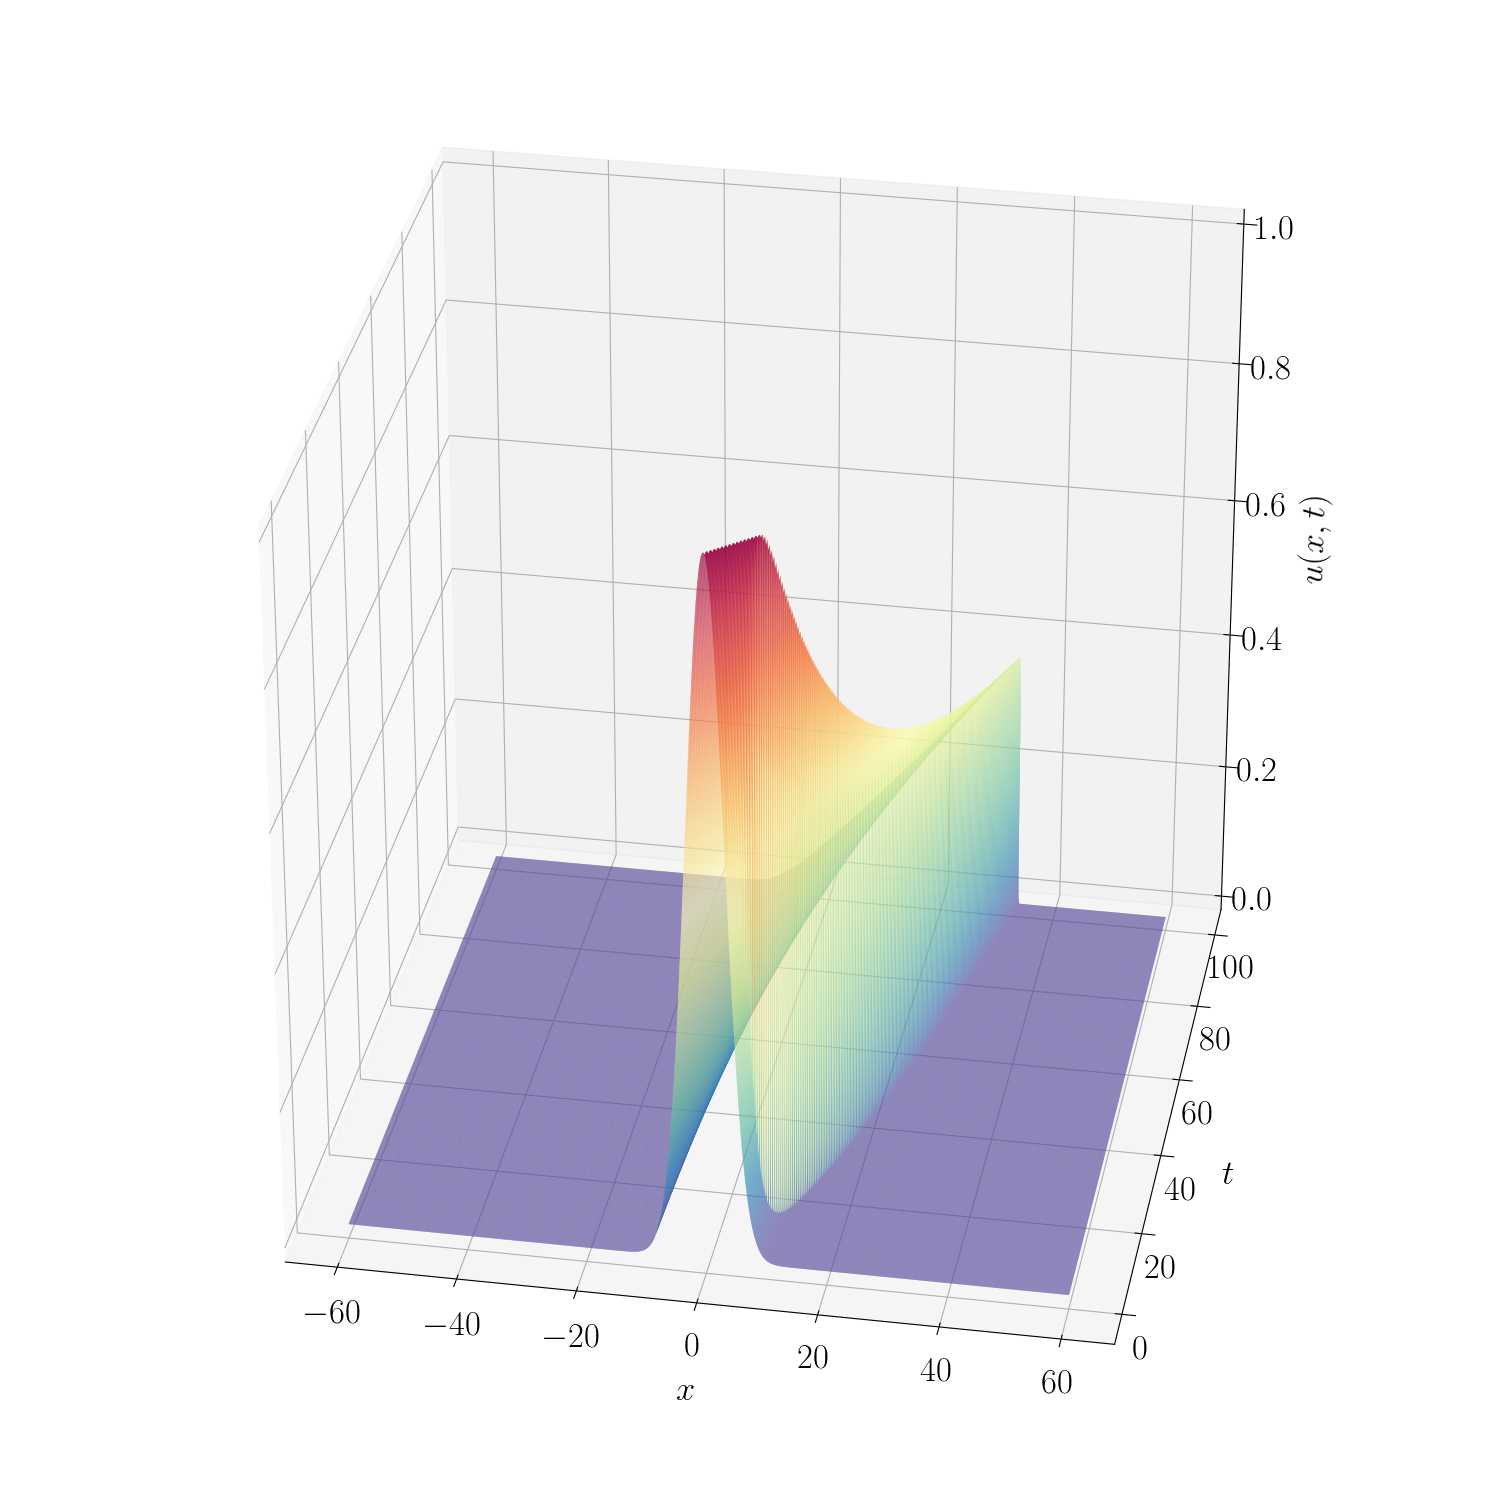
\includegraphics[width=11cm]{introduction/figures/Exact_Solution_alpha=001.png}
    	\caption{Exact solution for (\ref{IVP}) with initial condition $u_0 (x) = e^{-0.05x^2}$ using the equation (\ref{Exact_Solution}) for $x \in [-60, 60]$, $t \in [0, 100]$, and $\alpha = 0.01$.}
    	\label{Exact_Solution_alpha=0.01}
    \end{figure}
	\newpage
	\section{The Stochastic Burgers' equation}
     
    In real situations, the mathematical modeling of physical phenomena in a deterministic manner does not always produce satisfactory results, since certain hypotheses are established for their formulation, increasing uncertainty regarding spatial or temporal variables. To predict the behavior of a fluid, it is necessary to calculate the exact trajectory of each of the particles that compose it (which is an unapproachable problem). 
    
    When a fluid is in a closed container under pressure, each particle gets pushed against by all the surrounding particles. The container walls and the pressure-inducing surface (such as a piston) push against them in (Newtonian) reaction. These macroscopic forces are actually the net result of a very large number of intermolecular forces and collisions between the particles in those molecules. One fluid flow is isotropic if there is no directional preference (e.g. in fully developed turbulence); the kinetic theory of gases is also an example of isotropy if it's assumed that the molecules move in random directions and as a consequence, there is an equal probability of a molecule moving in any direction. 
    
    The equation given by (\ref{navierstokes}) assumes that the fluid is incompressible and isotropic, where the viscous stress is given by a linear relationship with the velocity gradient (Newton's viscosity law). In addition, the collective behavior of the fluid depends only on a few macroscopic variables (such as pressure, volume, and temperature) where the internal structure of the system and the individual behavior of the particles is not relevant for thermodynamic quantities. 
    
    Sometimes, due to the large size of such a system, quantum effects can be ignored and Newton's laws may be a good approximation (in some cases, if particles move very quickly with relativistic mechanics). But it is also possible to model a fluid as a set of randomly displaced point particles that do not interact with each other, analyzed by statistical mechanics.
    
    The information necessary to specify a physical system has to do with its entropy. When energy is degraded, Boltzmann said, it is because atoms assume a more disorderly state. And entropy is a parameter of disorder: that is the profound conception that emerges from Boltzmann's new interpretation. Oddly enough, you can create a measure for the disorder; is the probability of a particular state, defined here as the number of ways in which it can be assembled from its atoms. 
    
    When the interaction between the particles increases, their dispersion affects their positions and their velocities, which makes the entropy of the distribution increase over time until reaching a maximum (when the same system is as homogeneous and disorganized as possible). Then given a system of particles whose states $ X $ (usually position and velocity), it is possible to define a certain probability distribution that involves the various possible microstates of the system. The Maxwell-Boltzmann distribution shows how the speeds of the molecules are distributed in a Gaussian manner.
    
    The fundamental postulate of statistical mechanics, also known as a priori equiprobability postulate, says that given an isolated system in equilibrium, the system has the same probability of being in any of the accessible microstates. That is, a system in equilibrium has no preference for any of the microstates available for that balance. Then, in general, a system that ignores individual particles exhibits a global behavior that can be described statistically by defining macroscopic variables from a probability distribution over the microstates space.
    
    The basic concept of entropy in information theory has a lot to do with the uncertainty that exists in any random experiment or signal, which is also called the amount of "noise" or "disorder" that a system contains or releases. In this way, we can talk about the amount of information that a signal carries. Because of this, the idea of ​​implementing the Brownian movement, which represents the random movement observed in particles that are in a fluid medium (liquid or gas) as a result of collisions against the molecules of that fluid, gives us another way to describe complex fluids. 
        
    Over more than half a century a lot of deep mathematics was developed to tackle the rigorous understanding of turbulence and related questions in hydrodynamics problems. One of the approaches was to use stochastic analysis based on modifying the equations (as e.g. Euler, Navier-Stokes, and Burgers') adding a noise term. The idea here was to use the smoothing effect of the noise but also to discover new phenomena of stochastic nature on the other hand. In addition, this was also motivated by physical considerations, aiming at including perturbative effects, which cannot be modeled deterministically, due to too many degrees of freedom being involved, or aiming at taking into account different time scales to components of the underlying dynamics.
    
    Because Burgers' equation given by (\ref{Burgers_Equation}) has a unique solution for any initial condition given, it is not a good model for turbulence. It does not display any chaos; even when a force is added to the right-hand side all solutions converge to a unique stationary solution as time goes to infinity. However, developed a parallel, theoretical, and abstract mathematical beyond its dominant presence in applications. Motivated by the intention to reinstate the Burgers' equation as a model for turbulence, the community turned its attention to the randomly forced Burgers' equation.
    
    Several authors have suggested using the stochastic Burgers' equation as a simple model to study turbulence, \cite{Chambers1988,CHOI1992,DAH-TENC1969,HOSOKAWA1975}.
    In \cite{KARDAR1986} the stochastic burgers equation has been proposed to study the dynamics of the interfaces by adding a white noise (or Brownian motion) to the equation (\ref{Burgers_Equation}) on the right side, given as follows
    \begin{align}
    	\frac{\partial u(x, t)}{\partial t} = \alpha \frac{\partial^2 u(x, t)}{\partial x^2} + \frac{1}{2} \frac{\partial}{\partial x} (u^2 (x, t)) + \frac{\partial^2 \widetilde{W}}{\partial t \partial x}.
    	\label{stochastic_force} 
    \end{align}    
    This equation is a class of quasilinear stochastic PDEs (SPDEs), where $\widetilde{W} (x, t)$, $t \geq 0$, $x \in \mathbb{R}$ is a zero-mean Gaussian process. Moreover, we can write a cylindrical Wiener process $W$ by setting
    \begin{align*}
    	W(t) = \frac{\partial \widetilde{W}}{\partial x} = \displaystyle \sum_{j=1}^{\infty} \beta_j e_j,
    \end{align*}
    where ${e_j}$ is an orthonormal basis of $L_2 (0, 1)$ and ${\beta_j}$ is a sequence of mutually independent real Brownian motions in a fixed probability space $(\Omega, \mathcal{F}, \mathbb{P})$ adapted to a filtration $\{\mathcal{F}_t\}_{t \geq 0}$. For more details of the above, see the Appendix \ref{Appendix_A}.  
    
    \noindent In the following we shall write (\ref{stochastic_force}) as follows:
    \begin{align}
    	d X(\xi, t) = \left[ \alpha \partial_\xi^2 X(\xi, t) + \frac{1}{2} \partial_\xi \left(X^2 (\xi, t)\right) \right] dt + d W(\xi, t), \hspace{2mm} \xi \in [0, 1], \hspace{2mm} t > 0.
    	\label{burgers_stochastic}
    \end{align}
    Equation (\ref{burgers_stochastic}) is supplemented with Dirichlet boundary conditions
    \begin{align*}
    	X (0, t) = X (1, t) = 0, \hspace{2mm} \forall t \geq 0
    \end{align*}
    and the initial condition
    \begin{align*}
    	X(\xi, 0) = x(\xi), \hspace{2mm} \xi \in [0, 1] 
    \end{align*}
    
    The introduction of randomness in Burgers' equation produced a number of very interesting new directions; directions connected with dynamical systems aspects of the equation, e.g. existence and properties of invariant measures, directions related to various questions on the well-posedness of the equation in various functional settings using techniques from infinite-dimensional stochastic analysis. For further details see \cite{KARDAR1986} for instance.
    
    Also, during the past few decades, the stochastic Burgers' equation has found applications in diverse fields ranging from statistical physics, cosmology to fluid dynamics. The problem of Burgers' turbulence, that is the study of the solutions of Burgers' equation with random initial conditions or random forcing is a central issue in the study of nonlinear systems out of equilibrium. For further details see \cite{WEINAN, KHANIN2007} for instance.
    
    A main difficulty with the multidimensional stochastic Burgers equation is that the solutions take values in a distributional space, but in the case of one-dimension, the problem of existence of solutions for stochastic Burgers equation is well understood, see \cite{BERTINI1994, Catuogno2014, DAPRATO1994, PERKOWSKI2015}. 

\chapter{The Fundamental Theory For Spectral Methods}
\label{Chapter_2}
    
	\vspace{0.3cm}
	In this chapter, we will present the elements necessary to solve partial differential equations using spectral methods given as follows
	\begin{align}
	\label{general_problem}
	\left \lbrace \begin{array}{ll}
		&\frac{\partial u}{\partial t} = \mathcal{L} u, \hspace{3mm} x \in I, \hspace{3mm} t > 0,\\
		\\
		&u(x, 0) = g(x), \hspace{9mm} x \in I, 
		\end{array}  \right .
	\end{align}
	where $u$ is defined in some Hilbert space $\mathcal{H}$, with initial condition $g(x) \in \mathcal{H}$ and $\mathcal{L}$ is some spatial differential operator, which allows us to represent the previous problem in another whose solution $u$ will be given by a linear combination of already known functions. \\
	
	To do this, suppose that $\mathcal{H}$ is a separable Hilbert space with the inner product $\langle \cdot, \cdot \rangle$. Therefore, we can represent the function $u$ in terms of a known orthonormal base of $\mathcal{H}$, which we will denote as $\{\phi_k \}_{k \in I}$, given as follows 
	\begin{align*}
		\displaystyle u = \sum_{k \in I} \langle \phi_k, u \rangle \phi_k.
	\end{align*}
	
	There is a wide variety of families of base functions, which define different spectral methods. In this chapter, we will consider the well-known Fourier basis given by
	\begin{align}
		\label{base_phi}
		\phi_n (x) = e^{inx}.
	\end{align}
	that form an orthogonal set with the standard interior product $L^2$ in the interval $(0, 2 \pi)$, that is,
	\begin{align}
	\label{ortho_phi}
	\displaystyle \int_{0}^{2\pi} \phi_k (x) \overline{\phi_l (x)} dx = 2 \pi \delta{kl} = \left \lbrace \begin{array}{ll}
	0 \hspace{3mm} &\text{if} \hspace{3mm} k \neq l, \\
	2 \pi &\text{if} \hspace{3mm} k = l.
	\end{array}  \right.
	\end{align}
	
	We will denote as $B = span\{e^{inx}: |n| \leq \infty \}$ the set containing the Fourier bases. Therefore, we can define the Fourier series $F[u]$ for $u(x) \in L^2 [0, 2\pi]$ as follows 
	\begin{equation}
	\label{fourier_series}  
		F[u] \equiv \displaystyle \sum_{ |n| \leq \infty} \hat{u}_{n} e^{inx},
	\end{equation}
	where
	\begin{align}
	\label{coeff_fourier}
	\hat{u}_n = \frac{1}{2 \pi} \displaystyle \int_{0}^{2 \pi} u(x) e^{-inx} dx, \hspace{3mm}  k = 0, \pm 1, \pm 2, \dots.
	\end{align}
	which is known as the classical continuous series of trigonometric polynomials, where $\hat{u}_{n}$ are the Fourier coefficients. \\
    
    It is important noted that the integrals in (\ref{coeff_fourier}) exist if $u$ is Riemann-integrable, i.e., if $u$ is bounded and piecewise continuous in $(0, 2 \pi)$. More generally, the Fourier coefficients are defined for any function that is integrable in the Lebesgue sense. Also the relation (\ref{coeff_fourier}) associates with $u$ a sequence of complex numbers called the Fourier transform of $u$. It is possible as well to introduce a Fourier cosine transform and a Fourier sine transform of $u$, respectively, through the formulas
    \begin{align}
    \label{coeff_a_n}
    	a_n = \frac{1}{2 \pi} \displaystyle \int_{0}^{2 \pi} u(x) \cos(nx) dx, \hspace{3mm}  n = 0, \pm 1, \pm 2, \dots,
    \end{align}
    and
    \begin{align}
    \label{coeff_b_n}
    	b_n = \frac{1}{2 \pi} \displaystyle \int_{0}^{2 \pi} u(x) \sin(nx) dx, \hspace{3mm}  n = 0, \pm 1, \pm 2, \dots.
    \end{align}
    The three Fourier transforms of $u$ are related by the formula $\hat{u}_n = a_n - ib_n$ for $n = 0, \pm 1, \pm 2, \dots$. Moreover, if $u$ is a real valued function, $a_n$ and $b_n$ are real numbers, and $\hat{u}_{-n} = \hat{u}_n$. \\
	
	Based on the above, we will present two tools to build the methods that will be used in Chapter \ref{Chapter_3}, and that will be developed independently in the following two sections. In the first section, we will see that with the continuous Fourier expansion we can define a projection operator on a space of finite dimension that will allow us to approximate a function and its derivatives. In the second and last section, due to the complexity of the calculation of the previous integrals, we will see that it is possible to use quadrature rules to approximate them, and thus define an interpolation operator that will give us a discrete representation for a function and its derivatives.
	
	For these two operators, at the end of each section we will discuss the factors that determine the behavior of the series when used to approximate smooth functions, showing how fast they approach, when, and in what sense they are convergent.
	
	\newpage
	\section{Projection Operator: Continuous Fourier Expansion}
	\vspace{0.2cm}
		
	We define the projection operator denoted as $\mathcal{P}_N$ as the truncated Fourier series, i.e.,
	\begin{equation}
	\label{proyection_operator}
		\mathcal{P}_N u(x) \equiv  \displaystyle \sum_{ |n| \leq \frac {N}{2}} \hat{u}_{n} e^{inx}.
	\end{equation}	
	We will denote to $\hat{B}_N$ as the finite subset of $B = span\{e^{inx}: |n| \leq \infty \}$ on which it is projected the function, represented as follows
	\begin{align*}
		\hat{B}_{N} = span \left\{e^{inx}: |n| \leq \frac {N}{2} \right\},\hspace{0.2cm} dim(\hat{B}_{N}) = N + 1.
	\end{align*}
	Then by the orthogonality relation (\ref{ortho_phi}), it can be seen that for $u(x) \in L^2 [0, 2\pi]$
	\begin{align*}
		\langle \mathcal{P}_N u, v \rangle = \langle u, v \rangle, \hspace{3mm} \forall v \in S_N.
	\end{align*}
	This shows that $\mathcal{P}_N u$ is the orthogonal projection of $u$ upon the space of the trigonometric polynomials of degree $N$.\\
	
	Equivalently, $\mathcal{P}_N u$ is the closest element to $u$ in $\hat{B}_N$ with respect to the inner product
	\begin{align*}
		\langle u, v \rangle = \displaystyle \int_{0}^{2 \pi} u(x) \overline{v(x)} dx,
	\end{align*}
	and this also defines the norm
	\begin{align}
	\label{L2_dot}
		\| u \|^2 = \displaystyle \int_{0}^{2 \pi} |u(x)|^2 dx.
	\end{align}
	
	A full characterization of the functions for which the Fourier series is convergent is the framework of Lebesgue integration for convergence in mean. This convergence can be defined in $L^2 (0, 2 \pi)$ (square-integrable functions), also is a complex Hilbert space with inner product defined by (\ref{L2_dot}). Then for $u \in L^2 (0, 2 \pi)$ the Fourier series $F(u)$ given by (\ref{fourier_series}) is said to be convergent in mean (or $L^2$-convergent) to $u$ if
	\begin{align}
		\label{L2_mean}
		\displaystyle \int_{0}^{2 \pi} |u(x) - \mathcal{P}_N u(x) |^2 dx \rightarrow 0, \hspace{2mm} \text{as} \hspace{2mm} N \rightarrow \infty,
	\end{align}
	
	Then the Functions in $L^2 (0, 2 \pi)$ can be characterized in terms of their Fourier coefficients, according to the Riesz theorem, in the following sense. If $u \in L^2 (0, 2 \pi)$, then its Fourier series converges to $u$ in the sense of (\ref{L2_mean}), and by Parseval's identity show us that
	\begin{align}
	\label{parseval}
		\| u \|^2 = 2 \pi \displaystyle \sum^{\infty}_{-\infty} |\hat{u}_n|^2.
	\end{align}
	Conversely, if for any complex sequence $\{\hat{u}_n \}$, $n = 0, \pm 1, \dots $, and $\sum^{\infty}_{n=-\infty} |\hat{u}_n|^2 < \infty$, there exists a unique function $u \in L^2 (0, 2 \pi)$ such that its Fourier coefficients are precisely the $\hat{u}_n$$'$s for any $n$. Thus, for any function $u \in L^2 (0, 2 \pi)$ can be written as
	\begin{align}
		u = \displaystyle \sum^{\infty}_{n=-\infty} \hat{u}_n \phi_n.
	\end{align}
	
	The Riesz theorem states that the finite Fourier transform is an isomorphism between $L^2 (0, 2\pi)$ and the space $l^2$ of complex sequences $\{\hat{u}_n \}$, $n = 0, \pm1, \pm2, \dots$, such that $\sum^{\infty}_{n=-\infty} |\hat{u}_n|^2 < \infty$. The above can be summed up in the following theorem. 
	
	\begin{teor}
		 If the sum of squares of the Fourier coefficients is bounded
		\begin{align*}
			\displaystyle \sum_{ |n| \leq \infty} |\hat{u}_n|^2 < \infty
		\end{align*}
		then the truncated series converges in the $L^2$ norm
		\begin{align*}
			\|u -  \mathcal{P}_N u \|_{L^2 [0, 2\pi]} \rightarrow 0 \hspace{0.5cm} \text{as} \hspace{0.5cm} N \rightarrow \infty.
		\end{align*}
		If, moreover, the sum of the absolute values of the Fourier coefficients is bounded
		\begin{align*}
			\displaystyle \sum_{ |n| \leq \infty} |\hat{u}_n| < \infty
		\end{align*}
		then the truncated series converges uniformly 
		\begin{align*}
			\|u -  \mathcal{P}_N u \|_{L^{\infty} [0, 2\pi]} \rightarrow 0 \hspace{0.5cm} \text{as} \hspace{0.5cm} N \rightarrow \infty. 
		\end{align*}
	\end{teor}
	
	Note that if the truncated sum converges implies that the error is dominated by the tail of the series, i.e.,
	\begin{align*}
		\|u -  \mathcal{P}_N u \|^2_{L^2 [0, 2\pi]} = 2 \pi	\displaystyle \sum_{ |n| > \frac{N}{2} } |\hat{u}_n|^2,
	\end{align*}	
	and	
	\begin{align*}
		\|u -  \mathcal{P}_N u \|_{L^{\infty} [0, 2\pi]} \leq 
		\displaystyle \sum_{|n| > \frac{N}{2}} |\hat{u}_n|. 
	\end{align*}
	Thus, the error committed by replacing $u(x)$ with its $N$th-order Fourier series depends solely on how fast the expansion coefficients of $u(x)$ decay. \\
	
	To appreciate this, suppose that $u(x) \in L^2_p [0, 2 \pi]$ and that its derivative $u'(x) \in L^2_p [0, 2\pi]$, where the subscript $p$ indicate that the function is periodic. then for $n \neq 0$ we have to
	\begin{align*}
		2\pi \hat{u}_N &= \displaystyle \int_{0}^{2\pi} u(x) e^{-inx} dx \\
		&= - \frac{1}{in} (u(2\pi) - u(0)) - \frac{1}{in} \displaystyle \int_{0}^{2\pi} u'(x) e^{inx} dx, 
	\end{align*}
	therefore
	\begin{align*}
		|\hat{u}_N| \propto \frac{1}{n}.
	\end{align*}
	
	In general, if for $u(x)$ and its derivatives $(m - 1)$, and its periodic extensions are all continuous, and also if its derivative $m$th is measurable at $[0, 2 \pi]$, also known in the literature as the regularity of the function, in this particular case in $L^2_p$, we have to $\forall n \neq 0$, repeating the previous procedure successively, the behavior of Fourier coefficients $\hat{u}_n$ of $u(x)$ is similar, i.e.,
	\begin{align*}
		|\hat{u}_n| \propto \left(\frac{1}{n}\right)^m.
	\end{align*}
	
	 This is known as spectral convergence, which means that the smoother the function, the series converges faster.\\
	 
	 This result is important since it will allow us to investigate the convergence rate of the methods, which we will define in detail later. Therefore, we will focus on periodic functions expanded in Fourier series since its rapid decay of the coefficients implies that the Fourier series truncated after just a few more terms represents an exceedingly good approximation of the function. However, in practice, this decay is not exhibited until there are enough coefficients to represent all the essential structures of the function but in general, functions can be described both through their values in physical space and through their coefficients in transform space. The following examples illustrate the previous results. \\
	 
	\begin{example}
	    Consider the function $u(x) \in C^{\infty} [0, 2 \pi]$ given by
    	\begin{align}
    		\label{Example1} 
    	    u(x) = \frac{1}{5 - 4 \cos(x)}   
    	\end{align}
    	with its expansion coefficients
    	\begin{align*}
    	     \hat{u}_{n} = \frac{2^{-|n|}}{3}.
    	\end{align*}
    
    	In Figure \ref{fig1} we can clearly observe the convergence of the Fourier series and that in addition, the convergence of the approximation is almost uniform. This is due to the periodicity of the function and its derivatives.
    	
    	\begin{figure}[H]
        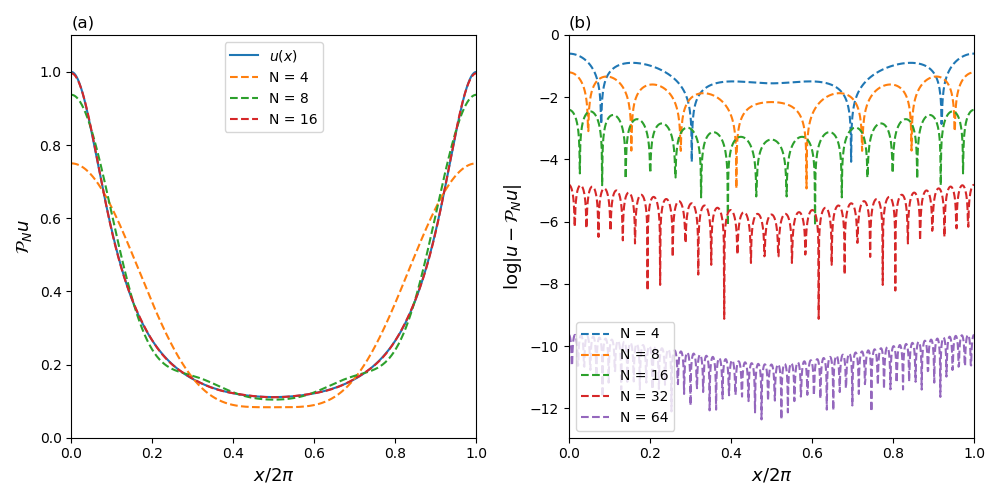
\includegraphics[width=\textwidth]{preliminaries/figures/example21.png}
        \caption{(a) Continuous Fourier series approximation of the equation (\ref{Example1}). (b) The Pointwise error of approximation.}
        \label{fig1}
        \end{figure}
	\end{example} 
	
	\begin{example}
	    The expansion coefficients of the function
    	\begin{align}
    		\label{Example2} 
    	    u(x) = \frac{\pi}{2} \sin(\frac{x}{2})
    	\end{align}
    	are given by
    	\begin{align*}
    	     \hat{u}_{n} = \frac{1}{(1 - 4n^2)}.
    	\end{align*}
    	
    	Note that is infinitely differentiable in $[0, 2 \pi]$, but $u'(0) \ne u' (2 \pi)$. In Figure \ref{fig2} we can see that the convergence is much slower than in the Example \ref{Example1}, as expected	
    	\begin{figure}[H]	
        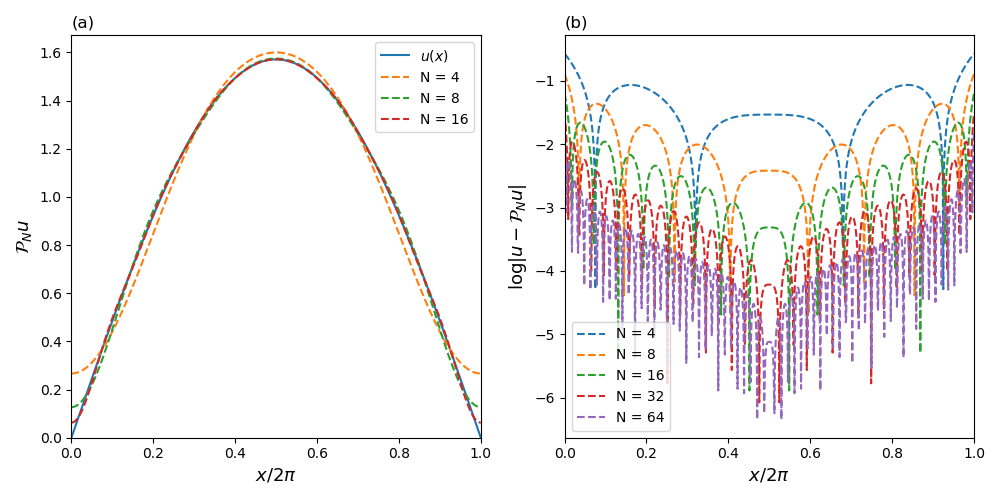
\includegraphics[width=\textwidth]{preliminaries/figures/example22.png}
        \caption{(a) Continuous Fourier series approximation of the equation (\ref{Example2}). (b) The Pointwise error of approximation for increasing resolution.}
        \label{fig2}
    	\end{figure}
	\end{example} 
	
	\subsection{Differentiation of the Continuous Expansion}

	To find solutions of partial differential equations using the spectral methods, in addition to approximating a function $u(x)$ by the finite Fourier series $\mathcal{P}_N u$, we also need to obtain its derivatives. Due to the linearity of the derivative and that these functions are exponential, we can easily obtain the derivatives of $\mathcal{P}_N u$ by simply differentiating the basis functions term by term. Therefore, if we have the following series truncated \\
 	\begin{align*}
   		\mathcal{P}_N u(x) =  \displaystyle \sum_{ |n| \leq \frac {N}{2}} \hat{u}_{n} e^{inx},
   	\end{align*}
    from this, we can get
   	\begin{align*}
   		\frac{d^q}{dx^q} \mathcal{P}_N u(x) = \displaystyle \sum_{ |n| \leq \frac {N}{2}} \hat{u}_{n} \frac{d^q}{dx^q} e^{inx} = \displaystyle \sum_{ |n| \leq \frac {N}{2}} (in)^q \hat{u}_{n}e^{inx}.
   	\end{align*}
    Therefore the projection and differentiation operators commute, i.e.,
    	\begin{align*}
    	\mathcal{P}_N \frac{d^q}{dx^q} u = \frac{d^q}{dx^q}\mathcal{P}_N u.
    	\end{align*}
    This property implies that for any differentiation operator $\mathcal{L}$ with constant coefficients,	
    	\begin{align*}
    	\mathcal{P}_N \mathcal{L} (I - \mathcal{P}_N)u
    	\end{align*}
     vanishes, which known as the truncation error. Thus, the Fourier approximation to the equation $u_t = \mathcal{L}u$ is exactly the projection of the analytic solution. 

    \subsection{Approximation theory for Continuous Expansion.}
    
    The behavior of the functions and their derivatives that we have shown is relevant when the solutions of the differential equations are approximated using spectral methods since it allows us to investigate how fast and precise they can be. In this subsection, we will present these properties based in \cite{gottlieb2007} as detailed as possible some useful results for our main objective regarding the analysis of the projection operator already defined above. \\
    
    When using the Fourier approximation to discretize the spatial part of the equation
    \begin{align*}
        u_t = \mathcal{L}u,
    \end{align*}
    it is important that our approximation, both to $u$ and to $\mathcal{L}u$, be accurate,i.e., we must consider not only the difference between $u$ and $\mathcal{P}_N u$ if not also the distance between $\mathcal{L} u$ and $\mathcal{L} \mathcal{P}_N u$, measured in an appropriate norm. This is because the actual rate of convergence is determined by the truncation error    
    \begin{align*}
    	\mathcal{P}_N \mathcal{L} (I - \mathcal{P}_N)u.
    \end{align*}
   	Thus, the error is determined not only by the behavior of the Fourier approximations of the function but also of its derivatives, as we have seen previously. Therefore, the Sobolev $q$-norm denoted by $H^q_p [0, 2\pi]$, It is appropriate to estimate the truncation error since it measures the smoothness of the derivatives and the function. This norm is defined as follows
    \begin{align}
    \label{sobolev_norm}
    	 \|u\|^2_{H^q_p [0, 2\pi]} = \displaystyle \sum^{q}_{m=0} \int^{2\pi}_{0} \left| u^m (x) \right|^2 dx.
    \end{align}
    The subscript $p$ indicates the fact that all functions are periodic. By substituting the Fourier expansion for each derivative in (\ref{sobolev_norm}), the Sobolev norm can be written as
    	\begin{align*}
    	    \|u\|^2_{H^q_p [0, 2\pi]} = 2\pi \displaystyle \sum^{q}_{m=0} \sum_{|n| \leq \infty} |n|^{2m} |\hat{u}_n|^2 = 2\pi \sum_{|n| \leq \infty} \left(\sum^{q}_{m=0} |n|^{2m} \right) |\hat{u}_n|^2,
    	\end{align*}
    where the interchange of the summation is allowed provided $u(x)$ has sufficient smoothness. \\
    
   Before starting the analysis, without loss of generality, we first consider the continuous Fourier series given by
        \begin{align*}
            \displaystyle \mathcal{P}_{2N} u(x) = \sum_{|n| \leq N} \hat{u}_n e^{in x}.
        \end{align*}
    The first important result is the estimate in $L^2$ for the distance between $u$ and its trigonometric approximation $\mathcal{P}_{2N} u$, which shows everything we've seen previously. 
    \\
    \begin{teor}
    \label{estimating_error_PN_L2}	
    For any $u(x) \in H_p^r [0, 2\pi]$, there exists a positive constant $C$, independent of $N$, such that
        \begin{align*}
    	    \|u - \mathcal{P}_{2N} u \|_{L^2 [0, 2\pi]} \leq C N^{-q} \|u^{(q)}\|_{L^2 [0, 2\pi]},
    	\end{align*}
    provided $0 \leq q \leq r$.
    \end{teor}
    \begin{proof}	
    By Parseval’s identity given by (\ref{parseval}) we get
    	\begin{align*}
    	    \|u - \mathcal{P}_{2N} u \|^2_{L^2 [0, 2\pi]} = 2\pi \displaystyle \sum_{|n| > N} |\hat{u}_n|^2.
    	\end{align*}
    We rewrite this summation as follows
    	\begin{align*}
    	    \displaystyle \sum_{|n| > N} |\hat{u}_n|^2 &= \sum_{|n| > N} \frac{n^{2q}}{n^{2q}} |\hat{u}_n|^2 \\
    	    &\leq N^{-2q} \sum_{|n| > N} n^{2q} |\hat{u}_n|^2 \\
    	    &\leq N^{-2q} \sum_{|n| \geq 0} n^{2q} |\hat{u}_n|^2 \\
    	    &= \frac{1}{2\pi} N^{-2q} \|u^{(q)}\|^2_{L^2 [0, 2\pi]}.
    	\end{align*}
    Putting all the above together and taking out the square root, we get our result.
	\end{proof}
    
    \noindent Note that the smoother the function, the larger the value of $q$ and therefore, the better the approximation, as seen before. Now let's notice the following. Suppose that $u(x)$ is analytical, so we have to
    	\begin{align*}
    		 u^{(q)} = \displaystyle 
    		 \sum_{ |n| \leq \infty} (in)^q \hat{u}_{n}e^{inx}.
    	\end{align*}
    Since $u^{(q)} \in W^q_p$, and by (\ref{parseval})
        \begin{align*}
            \|u^{(q)}\|_{L^2 [0, 2\pi]} = \sum_{ |n| \leq \infty} |n|^{2q} |\hat{u}_{n}|^2 \leq C q! \sum_{ |n| \leq \infty} |\hat{u}_{n}|^2 \leq C q! \| u \|_{L^2 [0, 2\pi]},
        \end{align*}
    and so by the previous theorem
        \begin{align*}
            \|u - \mathcal{P}_{2N} u \|_{L^2 [0, 2\pi]} \leq  N^{-q} \|u^{(q)}\|_{L^2 [0, 2\pi]} \leq C \frac{q!}{N^{q}} \| u \|_{L^2 [0, 2\pi]}.
        \end{align*}
    Using Stirling’s formula, $q! \sim q^q e^{-q}$, and assuming that $q \propto N$, we obtain
        \begin{align*}
            \|u - \mathcal{P}_{2N} u \|_{L^2 [0, 2\pi]} \leq \sim C \left(\frac{q}{N}\right)^q e^{-q} \| u \|_{L^2 [0, 2\pi]} \sim K e^{-c N} \| u \|_{L^2 [0, 2\pi]}.
        \end{align*}
    Thus, for an analytic function, its spectral convergence is exponential convergence. \\
    
    We must not forget that the theory we have previously presented is with the assumption that the functions and their derivatives are all periodic. But it is possible to do a similar analysis considering some other class of functions, such as functions that vanish at the borders. However, these kinds of functions belong to spaces very similar to those we have studied, and it is possible to use the same results.  
	
	\newpage
	\section{Interpolation Operator: Discrete Fourier Expansion}
    
    The continuous Fourier series method requires the evaluation of the coefficients
    \begin{align}
        \hat{u}_n = \displaystyle \frac{1}{2\pi} \int_{0}^{2\pi} u(x) e^{-inx} dx.
    \end{align}
    In general, these integrals cannot be computed analytically, and one resorts to the approximation of the Fourier integrals by using quadrature formulas. This procedure defines a discrete transform between the set of values of $u$ at the quadrature points and the set of approximate, or discrete, coefficients. The finite series defined by the discrete transform is actually the interpolate of $u$ at the quadrature nodes. If the properties of accuracy (in particular the spectral accuracy) are retained by replacing the finite transform with the discrete transform, then the interpolant series can be used instead of the truncated series to approximate functions. Also, quadrature formulas differ based on the exact position of the grid points, and the choice of an even or odd number of grid points results in slightly different schemes.
    
    \subsection{The Even Expansion}
    
    Define an equidistant grid, consisting of an even number $N$ of gridpoints $x_j \in [0, 2\pi)$, defined by
	\begin{align*}
        x_j = \frac{2 \pi j}{N} , \hspace{0.5cm} j\in [0, \cdots , N -1]. 
    \end{align*}
    The trapezoidal rule yields the discrete Fourier coefficients $\widetilde{u}_n$, which approximate the continuous Fourier coefficients $\hat{u}_n$ given as follows    
    \begin{align}
        	\widetilde{u}_n = \frac{1}{N}  \displaystyle \sum_{j = 0}^{N - 1} u(x_j) e^{-in x_j}.
    \end{align}
	The difference between the continuous and the discrete approximation is very clear since here we only need precision in the points $ x_j $. This may somehow be an advantage in the numerical calculation because in some cases it is possible to obtain the same order of precision, as shown in the following theorem when trigonometric polynomials are involved, the trapezoidal quadrature rule is a very natural approximation. \\
	
	\begin{teor}
	\label{Exactness_Even}	
	For the points $x_j$ defined as above, the quadrature formula
    \begin{align*}
         \frac{1}{2\pi}\displaystyle \int^{2\pi}_{0} f(x) dx = \frac{1}{N} \displaystyle \sum^{N-1}_{j=0} f(x_j), 
    \end{align*}
    is exact for any trigonometric polynomial $f(x) = e^{inx}$ , $|n| < N$.
    \end{teor}
	\begin{proof}
	Given a function $f(x) = e^{in x}$, It is easy to observe that
	
    \begin{align*}
        \frac{1}{2\pi}\displaystyle \int^{2\pi}_{0} f(x) dx =  \left \lbrace \begin{array}{ll}
    	1 \hspace{3mm} & \text{if } n = 0, \\
    	0 \hspace{3mm} & \text{otherwise.}
    	\end{array}  \right . 
    \end{align*}

	\noindent On the other hand,    
    \begin{align*}
        \frac{1}{N}  \displaystyle \sum_{j = 0}^{N - 1} f(x_j) &= \frac{1}{N}  \displaystyle \sum_{j = 0}^{N - 1} e^{in (\frac{2\pi j}{N})} \\
        &= \frac{1}{N}  \displaystyle \sum_{j = 0}^{N - 1} q^j
    \end{align*}
    where $q = e^{i \frac{2\pi n}{N}}$. If $n$ is an integer multiple of $N$ , i.e., $n = m N$, then, we have to
    \begin{align*}
    	\displaystyle \frac{1}{N} \sum^{N-1}_{j=0}  e^{i Nm (\frac{2\pi j}{N})} = \frac{1}{N} \sum^{N-1}_{j=0}  e^{i(2\pi j m)} = 1
    \end{align*} 
	Otherwise, 
	\begin{align*}
		\displaystyle \frac{1}{N} \sum^{N-1}_{j=0} q^j = \frac{q^{N} - 1}{q - 1} = 0
	\end{align*}
	Thus, the quadrature formula is exact for any function of the form $f(x) = e^{inx}$, $|n| < N$.
	\end{proof}

	Moreover, we can see that the quadrature formula is exact for $f(x) \in \hat{B}_{2N-2}$ where $\hat{B}_N$ is defined as before. Then using the trapezoid rule, the discrete Fourier coefficients become
	\begin{align}
	\label{coeficients_IN}
	    \widetilde{u}_n = \frac{1}{N \widetilde{c}_n}  \displaystyle \sum_{j = 0}^{N - 1} u(x_j) e^{-in x_j},
	\end{align}
	where we introduce the coefficients
	\begin{align}
	\label{constants_IN}	
	    \widetilde{c}_n = \left \lbrace \begin{array}{ll}
	    2  \hspace{0.25cm}\text{if} & |n| =  N/2, \\
	    \\
	    1  \hspace{0.25cm} \text{if} & |n| < N/2.
	\end{array}  \right .
	\end{align}

	\noindent These relations define a new projection of $u$
	\begin{equation}
	\label{collocation_operator_even}
		\mathcal{I}_N u(x) =  \displaystyle \sum_{ |n| \leq \frac {N}{2}} \widetilde{u}_n e^{inx}
	\end{equation}
	This is the complex discrete Fourier transform, based on an even number of quadrature points. From the above, we can see that
	\begin{align*}
	    \widetilde{u}_{-N/2} = \widetilde{u}_{N/2},
	\end{align*}
	so we have exactly $N$ independent Fourier coefficients, corresponding to the $N$ quadrature points. As a consequence, $\mathcal{I}_N \sin( \frac{N}{2} x) = 0$, so that the function $\sin( \frac{N}{2} x)$ is not represented in the above expansion. Therefore, the space $\hat{B}_N$ does not include $\sin( \frac{N}{2} x)$, and the correct space must be as follows
	\begin{align*}
	    \widetilde{B}_N = span\left\{\left(\cos(nx), \hspace{0.2cm} 0 \leq n \leq \frac{N}{2} \right)\cup  \left(\sin(nx), \hspace{0.2cm} 1 \leq n \leq \frac{N}{2} - 1 \right)\right\},
	\end{align*}
	which has dimension dim$(\widetilde{B}_N) = N$.\\
	
	\noindent In the same way, as in the previous subsection using the discrete expansion for Examples \ref{Example1} and \ref{Example2}, we can observe the same behavior as with continuous expansion, but now we have that the error at each point $x_j$ of the grid is zero.

	\begin{example}
	    Consider the $C^{\infty}_p [0, 2 \pi]$ function
    	\begin{align}
    		\label{Example4}
    	    u(x) = \frac{1}{5 - 4 \cos(x)}.
    	\end{align}
    	Its expansion coefficients are
    	\begin{align*}
    	     \hat{u}_{n} = \frac{2^{-|n|}}{3}.
    	\end{align*}
    	\begin{figure}[H]
        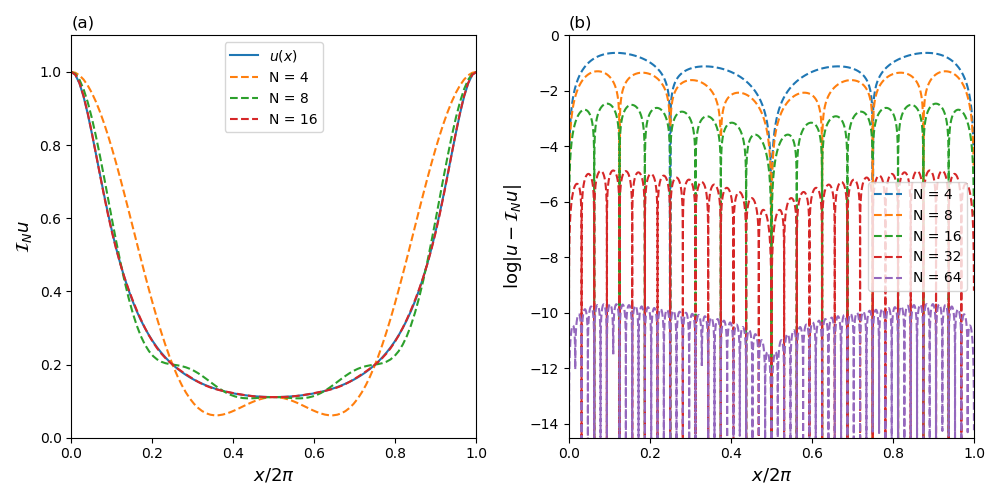
\includegraphics[width=\textwidth]{preliminaries/figures/example23.png}
        \caption{(a) Discrete Fourier series approximation of the equation (\ref{Example4}). (b) Pointwise error of approximation for increasing resolution.}
        \label{fig3}
        \end{figure}
	\end{example} 
	
	\begin{example}
	    The expansion coefficients of the function
    	\begin{align}
    		\label{Example5}
    	    u(x) = \frac{\pi}{2} \sin(\frac{x}{2}),
    	\end{align}
   		are given by
    	\begin{align*}
    	     \hat{u}_{n} = \frac{1}{(1 - 4n^2)}.
    	\end{align*}
    	\begin{figure}[H]
        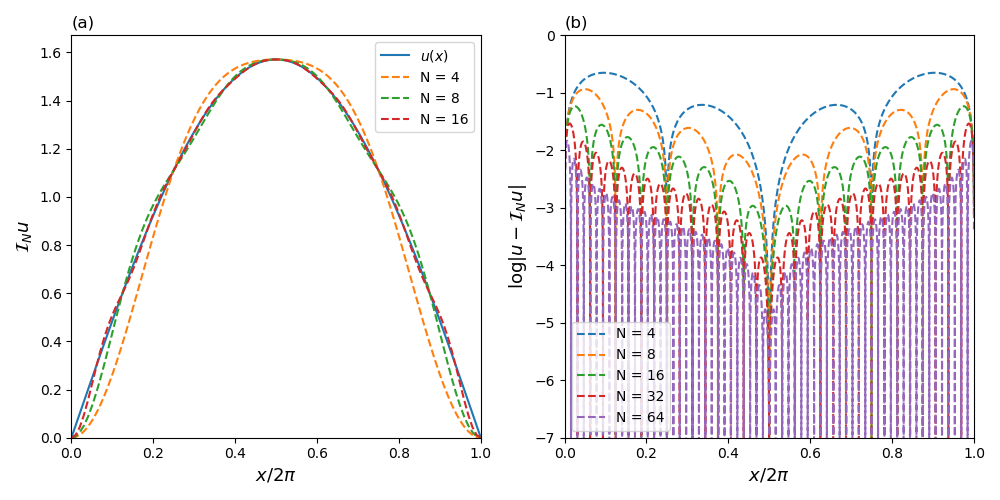
\includegraphics[width=\textwidth]{preliminaries/figures/example24.png}
        \caption{(a) Discrete Fourier series approximation of the equation (\ref{Example5}). (b) Pointwise error of approximation for increasing resolution.}
        \label{fig4}
        \end{figure}
	\end{example} 
	
	Therefore, we can see that the discrete expansion is, in fact, an interpolation operator as mentioned. This can be shown in the following theorem.\\
	
	\begin{teor}
	Let the discrete Fourier transform be defined by Equations (\ref{coeficients_IN})-(\ref{collocation_operator_even}). For any periodic function, $C^{0}_p [0, 2\pi]$, we have
	\begin{align*}
		\mathcal{I}_N u(x_j) = u(x_j), \hspace{0.3cm} \forall x_j = \frac{2 \pi j}{N} , \hspace{0.3cm} j = 0, \dots, N - 1. 
	\end{align*}
	\end{teor}

	\begin{proof}
	Substituting Equation (\ref{coeficients_IN}) into Equation (\ref{collocation_operator_even}) we obtain
	
	\begin{equation*}
    	\mathcal{I}_N u(x) =  \displaystyle \sum_{ |n| \leq \frac {N}{2}} \left(\frac{1}{N \widetilde{c}_n}  \displaystyle \sum_{j = 0}^{N - 1} u(x_j) e^{-in x_j}\right) e^{inx}.
	\end{equation*}
	Exchanging the order of the sum gives
	\begin{align}
	    \mathcal{I}_N u(x) = \displaystyle \sum_{j=0}^{N-1} u(x_j) g_j (x),
	\end{align}
	where
	\begin{align*}
	    g_j (x) &= \displaystyle \sum_{ |n| \leq \frac {N}{2}} \frac{1}{N \widetilde{c}_n} e^{in(x -x_j)}\\
	    &= \frac{1}{N} \sin\left[N \frac{x - x_j}{2} \right] \cot\left[\frac{x - x_j}{2} \right]
	\end{align*}
	by summing as a geometric series. It is easily verified that $g_j (x_i) = \delta_{ij}$\\
	\\
	We still need to show that $g_j (x) \in \widetilde{B}_N$. Clearly, $g_j (x) \in \hat{B}_N$ as $g_j (x)$ is a polynomial of degree $\leq N/2$. However, since
	
	\begin{align*}
	    \frac{1}{2} e^{-i \frac{N}{2} x_j} = \frac{1}{2} e^{i \frac{N}{2} x_j} = \frac{(-1)^j}{2},
	\end{align*}
	
	and, by convention $\widetilde{u}_{-N/2} = \widetilde{u}_{N/2}$, we do not get any contribution from the term $\sin(\frac{N}{2} x)$, hence $g_j (x) \in \widetilde{B}_N$.
	\end{proof}
	
	\subsection{The Odd Expansion}
	
	Similarly, we define a grid with an odd number of grid points as follows
	\begin{align*}
        x_j = \frac{2 \pi}{N + 1} j , \hspace{0.5cm} j\in [0, \dots , N],
    \end{align*}
    and using the trapezoidal rule we get
	\begin{align}
	\label{coefficients_JN}
        \widetilde{u}_n = \frac{1}{N + 1}  \displaystyle \sum_{j = 0}^{N} u(x_j) e^{-in x_j},
    \end{align}
    to obtain the interpolation operator
    \begin{equation}
    \label{Interpolation_operator_odd}
    	\mathcal{J}_N u(x) =  \displaystyle \sum_{ |n| \leq \frac {N}{2}} \widetilde{u}_n e^{inx}.
	\end{equation}
	
    \noindent Again as before, the quadrature formula is highly accurate. \\
    \begin{teor}
    \label{Exactness_Odd}	
    For the points $x_j$ defined as above, the quadrature formula
    \begin{align*}
         \frac{1}{2\pi}\displaystyle \int^{2\pi}_{0} f(x) dx = \frac{1}{N+1} \displaystyle \sum^{N}_{j=0} f(x_j),
    \end{align*}
    is exact for any $f(x) = e^{inx}$ , $|n| < N$, i.e., for all $f(x) \in \widetilde{B}_{2N}$.
    \begin{proof}
    	Given a function $f(x) = e^{in x}$, It is easy to observe that
    	
    	\begin{align*}
    		\frac{1}{2\pi}\displaystyle \int^{2\pi}_{0} f(x) dx =  \left \lbrace \begin{array}{ll}
    			1 \hspace{3mm} & \text{if } n = 0, \\
    			0 \hspace{3mm} & \text{otherwise.}
    		\end{array}  \right . 
    	\end{align*}
    	On the other hand,    
    	\begin{align*}
    		\frac{1}{N+1}  \displaystyle \sum_{j = 0}^{N} f(x_j) &= \frac{1}{N+1}  \displaystyle \sum_{j = 0}^{N} e^{in (\frac{2\pi j}{N+1})} \\
    		&= \frac{1}{N+1}  \displaystyle \sum_{j = 0}^{N} q^j
    	\end{align*}
    	where $q = e^{i \frac{2\pi n}{N+1}}$. If $n$ is an integer multiple of $N+1$ , i.e., $n = (N+1)m$, then we have to
    	\begin{align*}
    		\displaystyle \frac{1}{N+1} \sum^{N}_{j=0}  e^{i(N+1)m (\frac{2\pi j}{N+1})} = \frac{1}{N+1} \sum^{N}_{j=0}  e^{i (2\pi jm)} = 1
    	\end{align*}
    	 Otherwise, 
    	\begin{align*}
    		\displaystyle \frac{1}{N+1} \sum^{N}_{j=0} q^j = \frac{q^{N+1} - 1}{q - 1} = 0
    	\end{align*}
    	Thus, the quadrature formula is exact for any function of the form $f(x) = e^{inx}$, $|n| < N$.
    \end{proof}
    
    \end{teor}
    The scheme may also be expressed through the use of a Lagrange interpolation polynomial,
    \begin{align}
    \label{Lagrange_Odd}	
    	\mathcal{J}_N u(x) =  \displaystyle \sum_{j=0}^{N} u(x_j) h_j (x)
	\end{align}
	where
	\begin{align}
	    h_j (x) = \displaystyle \frac{1}{N+1} \sum_{|k| \leq \frac{N}{2}} e^{ik (x - x_j)} = \frac{1}{N + 1} \frac{\sin(\frac{N+1}{2}(x - x_j))}{\sin(\frac{x - x_j}{2})}
	\end{align}
    One easily shows that $h_j (x_l) = \delta_{jl}$ and that $h_j (x) \in \hat{B}_N $.
	
	\newpage
    \subsection{Differentiation of the discrete expansions}
    
    Similarly, as in continuous expansion, we require compute derivatives of the discrete approximation. In the following subsections, we assume that our function $u$ and all its derivatives are continuous and periodic on $[0, 2\pi]$.\\
    \\
    We consider the case of an even number of grid points. Using expansion coefficients given the values of the function $u(x)$ at the points $x_j$ , differentiating the basis functions in the interpolant yields
    \begin{align}
        \frac{d}{dx} \mathcal{I}_N u(x) = \displaystyle \sum_{|n| \leq N/2} in \widetilde{u}_n e^{inx}, \hspace{2mm} \widetilde{u}_n = \displaystyle \frac{1}{N \widetilde{c}_n} \sum_{j=0}^{N-1} u(x_j) e^{-in x_j},   
    \end{align}
    where $\widetilde{c}_n$ is given by (\ref{constants_IN}). Higher order derivatives can be obtained simply by further differentiating the basis functions.\\
    
    \noindent Similarly, for the case of an odd number of grid points
    \begin{align}
    	\frac{d}{dx} \mathcal{J}_N u(x) = \displaystyle \sum_{|n| \leq N/2} in \widetilde{u}_n e^{inx}, \hspace{2mm} \widetilde{u}_n = \displaystyle \frac{1}{N + 1} \sum_{j=0}^{N} u(x_j) e^{-in x_j},   
    \end{align} 
    The procedure for differentiating using expansion coefficients can be described as follows: first, we transform the point values $u(x_j)$ in physical space into the coefficients $\widetilde{u}_n$ in mode space. We then differentiate in mode space by multiplying  $\widetilde{u}_n$ by $in$, and return to physical space.\\
    
    There are other ways to obtain these derivatives, which may have greater advantage and be more efficient to calculate. In the literature, it can commonly find the use of differentiation matrices, for which there is a great variety. We will present some matrices that have been studied in \cite{gottlieb2007}, \cite{Canuto2012}, and we will observe the difference between the cases of an even and odd number of grid points. \\
    
    \paragraph{Differentiation Matrix.} Recall that to the case of an even number of grid points, the interpolation operator can be written as
    \begin{align*}
        \mathcal{I}_N u(x) = \displaystyle \sum^{N-1}_{j=0} u(x_j) g_j (x),
    \end{align*}
    where $g_j$ are the Lagrange interpolation polynomials given by
    \begin{align*}
        g_j (x) = \frac{1}{N} \sin\left[N \frac{x - x_j}{2} \right] \cot\left[\frac{x - x_j}{2} \right].
    \end{align*}
    Then, by differentiating the interpolation directly, it can get an approximation to the derivative of $u(x)$ at the points $x_j$ as follows
    \begin{align*}
        \displaystyle \frac{d}{dx} \mathcal{I}_N (x) \Big|_{x_l} = \sum^{N-1}_{j=0} u(x_j) \frac{d}{dx} g_j (x) \Big|_{x_l} = \sum^{N-1}_{j=0} D_{lj} u(x_j),
    \end{align*}
    where $D_{lj}$ are the differentiation matrix entries given by
    \begin{align}
    \label{matrix_DN_even}
        D_{ij} = \frac{d}{dx} g_j (x) \Big|_{x_i} = \begin{cases} \frac{(-1)^{i+j}}{2} \cot \left[ \frac{x_i - x_j}{2}\right] &   i \neq j, \\ \hspace{1mm} 0 &  i=j, \end{cases}
    \end{align}
    it is also well known that $D$ is circulant and skew-symmetric matrix. In the same way, the entries of the second order differentiation matrix $D^{(2)}$ gives us
    \begin{align}
    \label{matrix_D2N_even}
        D_{ij}^{(2)} = \frac{d^2}{dx^2} g_j (x) \Big|_{x_i} = \begin{cases} -\frac{(-1)^{i+j}}{2} \left[\sin \left[ \frac{x_i - x_j}{2}\right]\right]^{-1} &   i \neq j, \\ -\frac{N^2 + 2}{12} &  i=j. \end{cases}
    \end{align}
	
    The approximation of higher derivatives follows exactly the same route, and similarly to obtain the entries of the differentiation matrix $\widetilde{D}$ for the interpolation based on an odd number of points given by
    \begin{align}
    \label{matrix_DN_odd}
        \widetilde{D}_{ij} = \begin{cases} -\frac{(-1)^{i+j}}{2} \left[\sin \left[ \frac{x_i - x_j}{2}\right]\right]^{-2} &   i \neq j, \\ \hspace{1mm} 0 &  i=j. \end{cases}
    \end{align}

    It is also known that $\widetilde{D}$ is a circulant, skew-symmetric matrix. The advantage of this method is that the differentiation matrix takes us from physical space to physical space, and the act of differentiation is hidden in the matrix itself. \\
    
    It is interesting to observe that the differentiation operator for the interpolation based on an odd number of grid points, takes elements of $\widetilde{B}_N$ out of $\widetilde{B}_N$ and then
    \begin{align*}
    	\mathcal{I}_N \frac{d^2}{dx^2} \mathcal{I}_N \neq \left( \mathcal{I}_N \frac{d}{dx} \right)^2 \mathcal{I}_N.
    \end{align*}
	
	But for the interpolation based on an odd number of grid points the differentiation operator remain in $\hat{B}_N$ when takes elements of $\hat{B}_N$, and thus,
	\begin{align*}
		\mathcal{J}_N \frac{d^2}{dx^2} \mathcal{J}_N = \left( \mathcal{J}_N \frac{d}{dx} \right)^2 \mathcal{J}_N
	\end{align*}
    Moreover, for all values of $q$ we have
    \begin{align*}
        \widetilde{D}^{(q)} = \mathcal{J}_N \frac{d^q}{dx^q} \mathcal{J}_N = \widetilde{D}^q
    \end{align*}
	allowing us to calculate approximate high derivatives by just multiplying the $D$ matrix as many times as necessary.
    
    For the above, and for some interesting properties that we will see later about interpolation operator based on an odd number of grid points, it has been decided to use it for the study of this work.
    
    \subsection{Approximation theory for Discrete Expansion.}
    
    Based on the theory developed in \cite{gottlieb2007} with respect to the interpolation operator analysis for the case of an even number of grid points, we will adapt the results for the case of an odd number of grid points in the most detailed way possible. \\
    
    \noindent First of all, we can define a discrete version of the inner product $L^2$ as follows
    \begin{align*}
    	\langle f_N, g_N \rangle_N = \displaystyle \frac{1}{N + 1} \sum_{j = 0}^{N} f_N (x_j) \bar{g}_N (x_j),
    \end{align*}
	and the associated norm
	\begin{align*}
		\| f_N \|_N^2 = \langle f_N, f_N \rangle_N
	\end{align*}
	where $f_N$ , $g_N \in \hat{B}_N$ and there are an odd number of grid points $x_j$ , $j = 0, \dots , N$. Note also that the interpolant $\mathcal{J}_N u$ of a continuous function $u$ and for all $v \in \hat{B}_N$, satisfies trivially the identity
	\begin{align*}
		\langle \mathcal{J}_N u, v \rangle_N = \langle u, v \rangle_N.
	\end{align*} 
	
	Moreover, as a consequence of the exactness of the quadrature rule for trigonometric functions, as have seen in Theorem \ref{Exactness_Even}, we have
	\begin{align}
	\label{Coincidence_Inner}	
		\langle f_N, g_N \rangle_N = \displaystyle \frac{1}{2 \pi} \int_{0}^{2 \pi} f_N \bar{g}_N dx, \hspace{3mm} \|f_N\|_{L^2 [0, 2 \pi]} = \|f_N\|_N
	\end{align}

	Hence, in $\hat{B}_N$ , the continuous and discrete inner product are the same.\\
	
	The situation is different when we discuss an even number of grid points. If $f_N , g_N \in \tilde{B}_N$ and we have an even number of grid points $x_j$ , the discrete inner product
	\begin{align*}
		\langle f_N, g_N \rangle_N = \displaystyle \frac{1}{N} \sum_{j = 0}^{N - 1} f_N (x_j) \bar{g}_N (x_j), \hspace{3mm} \|f_N\|_N^2 = \langle f_N, f_N \rangle_N
	\end{align*}
	is not equal to the continuous inner product. However, using the fact that $f_N \in L^2 [0, 2 \pi]$ it can be shown that there exists a $K > 0$ such that
	\begin{align}
	\label{equivalent_discrete_continous}
		K^{-1} \|f_N\|^2_{L^2 [0, 2 \pi]} \leq \|f_N\|^2_N \leq K \|f_N\|^2_{L^2 [0, 2 \pi]}.
	\end{align}
    
    Something very interesting and useful in the use of discrete expansion to approximate functions and their derivatives is that the behavior is very similar to that shown in the previous subsection for continuous expansion. We will see that the approximation theory for the discrete expansion yields essentially the same results as for the continuous expansion. The proofs are based on the fact that the Fourier coefficients of the discrete approximation are sufficiently close to those of the continuous approximation. \\
    
    Recall that the interpolation operator associated with an odd number of grid points is given by
    \begin{align*}
    	\mathcal{J}_{2N} u = \displaystyle \sum_{|n|\leq N} \widetilde{u}_n e^{inx},
    \end{align*}
    with expansion coefficients
    \begin{align*}
    	\widetilde{u}_n = \displaystyle \frac{1}{2N + 1} \sum^{2N}_{j=0} u(x_j)e^{-in x_j}, \hspace{2mm} x_j = \frac{2 \pi j}{2N+1}.
    \end{align*}
    
    First we observe the following, the interpolation operator associated with an odd number of grid points are based on the points $x_j$, for which the $(n + Mm)$th mode, where $M = 2N + 1$, is indistinguishable from  the $n$th mode, i.e.,
    \begin{align*}
    	e^{i(n + Mm)x_j} = e^{in x_j} e^{i 2 \pi m j} = e^{in x_j}
    \end{align*}
	This phenomenon is known as aliasing.\\
	
	Moreover, due to the orthogonality relation as before seen we have to
    \begin{align*}
    	\frac{1}{M} \displaystyle \sum^{M-1}_{j=0} e^{-inx_j} =  \left \lbrace \begin{array}{ll}
    	1 \hspace{4mm} &\text{if} \hspace{2mm} n=M m, \hspace{2mm} m = 0, \pm 1, \pm 2, \dots, \\
    	0 &\text{otherwise.}
    	\end{array}  \right .
    \end{align*} 
    
    The relationship between the discrete expansion coefficients $\widetilde{u}_n$ , and the continuous expansion coefficients $\hat{u}_n$, is given in the following lemma. 
    
    \begin{lemma}
    \label{lemma_2.1}
    Consider $u(x) \in W^q_p [0, 2\pi]$, where $q > 1/2$. For $|n| \leq N$ we have
	    \begin{align}
	    \label{alias}   
	        \widetilde{c}_n \widetilde{u}_n = \displaystyle \hat{u}_n + \sum_{\substack{|m|\leq \infty \\ m \neq 0}} \hat{u}_{n + Mm}
	    \end{align}
	\end{lemma}
	\begin{proof}
    Substituting the continuous Fourier expansion into the discrete expansion yields
    \begin{align*}
        \widetilde{c}_n \widetilde{u}_n = \frac{1}{M} \displaystyle \sum_{j=0}^{M - 1} \sum_{|l| \leq \infty} \hat{u}_l e^{i(l -n)x_j}
    \end{align*}
    To interchange the two summations we must ensure uniform convergence, i.e., $\sum_{|l| \leq \infty} |\hat{u}_l| < \infty$. This is satisfied, since if $q> 1/2$ then, as before there is $m \in \mathbb{N}$ such that for $l \geq m$ we have to
    \begin{align*}
    	(1 + |l|)^{2q} \leq 2q(1 + l^{2q}) 
    \end{align*}
	taking $m$ as follows 
	\begin{align*}
		\frac{1}{m} \leq (2q)^{\frac{1}{2q}} - 1 
	\end{align*}

	\noindent Therefore
    \begin{align*}
        \displaystyle \sum_{|l| \leq \infty} |\hat{u}_l| &= \sum_{|l| \leq \infty} (1 + |l|)^q \frac{|\hat{u}_l|}{(1 + |l|)^q}  \\
        &\leq \left( 2q \sum_{|l| \leq \infty}  (1 + l^{2q}) |\hat{u}_l|^2 \right)^{1/2} \left(\sum_{|l| \leq \infty} (1 + |l|)^{-2q}  \right)^{1/2},
    \end{align*}
    where the last expression follows from the Cauchy-Schwarz inequality. As $u(x) \in W^q_p [0, 2\pi]$ the first part is clearly bounded. Furthermore, the second term is a $p$-series and then converges provided $q > 1/2$, ensuring boundedness. \\
    
    Interchanging the order of summation and using orthogonality of the exponential function at the grid yields the desired result
    \begin{align*}
    	\widetilde{c}_n \widetilde{u}_n &= \frac{1}{M} \displaystyle \sum_{j=0}^{M - 1} \sum_{|l| \leq \infty} \hat{u}_l e^{i(l -n)x_j} =  \sum_{|l| \leq \infty} \frac{1}{M} \sum_{j=0}^{M - 1} \hat{u}_l e^{i(l -n)x_j} \\
    	&= \sum_{|m| \leq \infty}  \frac{1}{M} \sum_{j=0}^{M - 1} \hat{u}_{n + Mm} e^{i(n + Mm)x_j} \\
    	&= \frac{1}{M} \sum_{j=0}^{M - 1} \hat{u}_n e^{inx_j}
    	+ \sum_{\substack{|m|\leq \infty \\ m \neq 0}} \frac{1}{M} \sum_{j=0}^{M - 1} \hat{u}_{n + Mm} e^{i(n + Mm)x_j} \\
    	&= \hat{u}_n + \sum_{\substack{|m|\leq \infty \\ m \neq 0}} \hat{u}_{n + Mm}
    \end{align*}
	\end{proof}
	
	The conclusions of the previous discussion are equally valid in the number of odd or even points. An equivalent formulation of (\ref{alias}) is
	\begin{align*}
		\mathcal{J}_N u = \mathcal{P}_N u + \mathcal{A}_N u
	\end{align*}
	It is orthogonal to the truncation error, $u - \mathcal{P}_N u$, so that
	\begin{align*}
		\| u - \mathcal{J}_N u \|^2 = \|u - P_N u \|^2 + \| \mathcal{A}_N u \|^2
	\end{align*}
	Hence, the error due to the interpolation is actually always larger than the error due to the truncation of the Fourier series.\\
	
	Rather than deriving the estimates of the approximation error directly, we shall use the results obtained in the previous section and then estimate the difference between the two different expansions, which we recognize as the aliasing error given by
	\begin{align*}
		\| \mathcal{A}_N \|_{L^2 [0, 2\pi]} = \left\| \displaystyle \sum_{|n|<N} \left( \sum_{\substack{|m|\leq \infty \\ m \neq 0}} \hat{u}_{n + Mm}  \right) \right\|_{L^2 [0, 2\pi]}
	\end{align*}
    
    As before, we first consider the behavior of the approximation in the $L^2$-norm. We will first show that the bound on the aliasing error, $\mathcal{A}_N$ , in equation above is of the same order as the truncation error. The error caused by truncating the continuous expansion is essentially the same as the error produced by using the discrete coefficients rather than the continuous coefficients.
    \begin{lemma}
    \label{estimating_aliasing_error}	
    For any $u(x) \in W_p^r [0, 2\pi]$, where $r > 1/2$, the aliasing error
    \begin{align*}
        \| \mathcal{A}_N \|_{L^2 [0, 2\pi]} = \displaystyle \left(\sum_{|n| \leq \infty} |\widetilde{c}_n \widetilde{u}_n - \hat{u}_n|^2 \right)^{1/2} \leq CN^{-r} \|u^{r}\|_{L^2 [0, 2\pi]}
    \end{align*}
	\end{lemma}
	\begin{proof}
    From Lemma \ref{lemma_2.1} we have
    \begin{align*}
        |\widetilde{c}_n \widetilde{u}_n - \hat{u}_n|^2 = \displaystyle \left|\sum_{\substack{|m|\leq \infty \\ m \neq 0}} \hat{u}_{n + Mm} \right|^2
    \end{align*}
    To estimate this, we first note that
    \begin{align*}
        \displaystyle \left|\sum_{\substack{|m|\leq \infty \\ m \neq 0}} \hat{u}_{n + Mm} \right|^2 &= \left|\sum_{\substack{|m|\leq \infty \\ m \neq 0}} |n + Mm|^r \hat{u}_{n + Mm} \frac{1}{|n + Mm|^r} \right|^2 \\ 
        &\leq \left(\sum_{\substack{|m|\leq \infty \\ m \neq 0}} |n + Mm|^{2r} |\hat{u}_{n + Mm}|^2 \right) \left(\sum_{\substack{|m|\leq \infty \\ m \neq 0}} \frac{1}{|n + Mm|^{2r}}  \right)
    \end{align*}
    using the Cauchy-Schwartz inequality. Since $M =2N + 1$ and  $|n| \leq N$, we have to $N(2m - 1) = 2Nm - N \leq |n + Mm|$. Hence, bounding of the second term is ensured by
    \begin{align*}
        \displaystyle \sum_{\substack{|m|\leq \infty \\ m \neq 0}} \frac{1}{|n + Mm|^{2r}} \leq \frac{2}{N^{2r}} \sum^{\infty}_{m=1} \frac{1}{(2m - 1)^{2r}} = C_1 N^{-2r},
    \end{align*}
    provided $r > 1/2$. Here, the constant $C_1$ is a consequence of the fact that the power series converges, and it is independent of $N$.\\
    Summing over $n$, we have
    \begin{align*}
        \displaystyle \sum_{|n|\leq N} \left|\sum_{\substack{|m|\leq \infty \\ m \neq 0}} \hat{u}_{n + Mm} \right|^2 &\leq \sum_{|n| \leq N} C_1 N^{-2r} \sum_{\substack{|m|\leq \infty \\ m \neq 0}} |n + Mm|^{2r} |\hat{u}_{n + Mm}|^2 \\
        &\leq C_2 N^{-2r} \| u^{(r)} \|^2_{L^2[0, 2\pi]}
    \end{align*}
	\end{proof}

    We are now in a position to state the error estimate for the discrete approximation.
    \begin{teor}
    \label{estimating_error_I_N_L2}	
    For any $u(x) \in W_p^r [0, 2\pi]$ with $r > 1/2$, there exists a positive constant $C$, independent of $N$ , such that
    \begin{align*}
        \| u - \mathcal{J}_{2N}u \|_{L^2 [0, 2\pi]} \leq CN^{-r} \| u^{(r)} \|_{L^2 [0, 2\pi]}
    \end{align*}
	\end{teor}
    \begin{proof}
    Let’s write the difference between the function and its discrete approximation
    \begin{align*}
        \| u - \mathcal{J}_{2N}u \|_{L^2 [0, 2\pi]} &= \| (\mathcal{P}_{2N} - \mathcal{J}_{2N})u + u - \mathcal{P}_{2N}u \|_{L^2 [0, 2\pi] } \\
        &\leq  \| (\mathcal{P}_{2N} - \mathcal{J}_{2N})u \|_{L^2 [0, 2\pi] } + \| u - \mathcal{P}_{2N}u \|_{L^2 [0, 2\pi] }
    \end{align*}
    Thus, the error has two components. The first one, which is the difference between the continuous and discrete expansion coefficients, is the aliasing error, which is bounded in Lemma \ref{estimating_aliasing_error}. The second, which is the tail of the series, is the truncation error, which is bounded by the result of Theorem \ref{estimating_error_PN_L2}. The desired result follows from these error bounds.
	\end{proof}

    Theorem above confirms that the approximation errors of the continuous expansion and the discrete expansion are of the same order, as long as $u(x)$ has at least half a derivative. Furthermore, the rate of convergence depends, in both cases, only on the smoothness of the function being approximated.   	

\chapter{Solutions for Burgers' Equation in the Deterministic Version}
\label{Chapter_3} 
	
	This chapter is one of the most important, since we will begin with the development of the main objective of this work. We will construct two spectral methods known as Fourier-Galerkin and Fourier-Collocation using the projection and interpolation operators respectively, considering an initial value problem that will be defined using our objective equation presented in (\ref{Burgers_Equation}). \\
	
	For this, to illustrate what we have studied in the Chapter (\ref{Chapter_2}), we will consider the function space $H^q_p [0, 2 \pi]$ with the norm defined in (\ref{sobolev_norm}) for some $q$ that will be specified later. We will assume that the problems have solutions $u(x, t) \in H^q_p [\mathcal{D}]$ for every $t \in I$, where $\mathcal{D} = [x_L, x_R]$ for some fixed reals $ x_L $, $ x_R $ and $I = [0, T]$ with $T> 0$. So, given some real $\alpha \geq 0$ and an initial condition function $u_0 (x) \in H^q_p [\mathcal{D}]$, our initial value problem is as follows
	\begin{align}
	\label{IVP_Burgers}
		\left \lbrace \begin{array}{ll}
			\frac{\partial u}{\partial t} + \frac{1}{2} (u^2)_x = \alpha \frac{\partial^2 u}{\partial x}, \hspace{2mm} 0 < t \leq T, \hspace{2mm} x \in I \\
			\\
			u(x, 0) = u_0(x), \hspace{2mm} x \in I
		\end{array}  \right .
	\end{align}
	
	The analytical solution of the previous problem was given in (\ref{Exact_Solution}), and we observe that it is not easy to evaluate it directly. Therefore, it is necessary to choose a suitable method of numerical integration to calculate the integrals involved, since they have exponential behavior that is noticeably affected when the parameter $\alpha$ is very small. However, precision problems can also arise because arithmetic operations can generate considerable errors if they are not performed correctly, and therefore this equation is not a good choice for finding solutions to the problem. \\
	
	In the next section, we will present the aforementioned spectral methods considering the linear problem obtained by using the transformation given by (\ref{Hopf_tranform}), And this will allow us to approximate the solutions of the problem (\ref{IVP_Burgers}) More easily and with excellent precision. In addition, this will give us the advantage of having solutions that can be considered exact and use them to compare them with those that will be obtained in the numerical experiments that we will describe in the second section when implementing these methods for the nonlinear problem (\ref{IVP_Burgers}), Since we will observe that the precision will be much less because we will need to use numerical methods to solve in the variable $t$, decreasing with respect to the parameter $\alpha$.
    
	\section{Fourier Spectral Methods}
	
	In the following sections we will work with the problem obtained by the transformation of the problem (\ref{Hopf_tranform}) given by
	\begin{align}
		u(x, t) = - 2 \alpha \frac{\partial_{x} \varphi(x, t)}{\varphi(x, t)} = - 2 \alpha \left( \log{\varphi(x, t)} \right)_x
	\end{align}
	with $\alpha > 0$, and $\varphi$ solves the following initial value problem
	\begin{align}
	\label{Bugers_Lineal}	
		\left \lbrace \begin{array}{ll}
			\frac{\partial \varphi}{\partial t} = \alpha \varphi_{xx}, \hspace{2mm} 0 < t \leq T, \hspace{2mm} x \in I \\
			\\
			\varphi(x, 0) = \displaystyle \varphi_0 (x) = e^{- \int_{0}^{x} \frac{u_0(y)}{2 \alpha} dy}, \hspace{2mm} x \in I
		\end{array}  \right .
	\end{align}
	\subsection{Fourier-Galerkin}
    \label{Galerkin}
	\vspace{0.3cm} 
	
	
	In chapter \ref{Chapter_2} we saw that for a function $\varphi \in H^2_p [0, 2 \pi]$ it can be written as
	\begin{align}
	\label{Expansion_phi}	
		\varphi (x, t) = \displaystyle \sum_{|n| \leq \infty} \hat{\varphi}_n (t) \phi_n (x), \hspace{2mm} \hat{\varphi}_n (t) = \frac{1}{2 \pi} \left\langle \varphi (x, t), \phi_n (x) \right\rangle  
	\end{align}
	where $\phi_n (x) = e^{inx}$, and let's assume that this function is the solution of the problem (\ref{Bugers_Lineal}).\\
	
	The Fourier-Galerkin method will be constructed using the project operator described in (\ref{proyection_operator}) to project and force the function $\varphi$ to satisfy the problem (\ref{Bugers_Lineal}) on a space that will be defined a continuation. \\
	
	Let $V_N$ the space of trigonometric polynomials of degree $2N + 1$ given by $V_N = B_N \cap H^2_p [0, 2 \pi]$, where $B_N = span\{\phi_n (x) : |n| \leq N\}$. Then for $\varphi \in V_N$ we can obtain its expansion as  
	\begin{align}
	\label{Expansion_phi_N}	
		\varphi_N (x, t) = \displaystyle \sum_{|n| \leq N} \hat{\varphi}_n (t) \phi_n (x), \hspace{2mm} \hat{\varphi}_n (t) = \frac{1}{2 \pi} \left\langle \varphi (x, t), \phi_n (x) \right\rangle  
	\end{align} 
	
	Substituting (\ref{Expansion_phi}), and (\ref{Expansion_phi_N}) into the equation (\ref{Bugers_Lineal}) to taking the difference as follows
	\begin{align*}
		\left[ \frac{\partial}{\partial t} \varphi_N - \alpha \frac{\partial^2}{\partial x} \varphi_N \right] - \left[ \frac{\partial \varphi}{\partial t} - \alpha \frac{\partial^2 \varphi}{\partial x} \right] = R_N (x, t)   
	\end{align*}
	where $R_N (x, t)$ is a residual function, and since the second term is exactly zero because $\varphi$ is the exact solution we have to
	\begin{align*}
		\frac{\partial}{\partial t} \varphi_N -  \alpha \frac{\partial^2}{\partial x} \varphi_N = R_N (x, t)
	\end{align*}
	
	In the Fourier-Galerkin method, it is desired that the remainder $R_N$ belong to the orthogonal space of $ V_N $, that is, for every $\varphi, \phi \in V_N $ such that $\langle \varphi - \mathcal{P}_N \varphi, \phi \rangle = 0$. This is achieved by forcing for each $|n| \leq N$ the following condition
	\begin{align}
		\left\langle R_N, \phi_n \right\rangle = \left\langle \frac{\partial \varphi_N}{\partial t} - \alpha \frac{\partial^2 \varphi_N}{\partial x^2}, \phi_n \right\rangle = 0, \hspace{2mm}  \hspace{2mm} \phi_n \in V_N, \hspace{2mm} \forall t > 0
	\end{align}
	or equivalently
	\begin{align*}
		\displaystyle \int_{\mathcal{D}} \frac{\partial}{\partial t} \varphi_N (x, t) \overline{\phi_n (x)} dx = \alpha \int_{\mathcal{D}} \frac{\partial^2}{\partial x^2} \varphi_N (x, t) \overline{\phi_n (x)} dx , \hspace{2mm}  \hspace{2mm} \phi_n \in V_N, \hspace{2mm} \forall t > 0
	\end{align*}
	
	\noindent Using the orthogonality $\langle \phi_k, \phi_n \rangle = 2 \pi \delta_{kn}$, for each $n$ fixed we have to
	\begin{align*}
		\left\langle \frac{\partial \varphi_N}{\partial t}, \phi_n  \right\rangle = \left\langle \displaystyle \sum_{ |k| \leq N} \frac{d \hat{\varphi}_k (t)}{dt} \phi_k, \phi_n  \right\rangle = 2 \pi \frac{d \hat{\varphi}_n (t)}{dt}
	\end{align*}
	
	Note that the spatial interval is not the desired one, for this we are going to define the following linear transformation from $\mathcal{D}_p = [0, 2 \pi]$ to $\mathcal{D} = [x_L, x_R]$ given by $x = P z + x_L$ to escalate the problem, where $P = \frac{x_R - x_L}{2 \pi}$ and $z \in \mathcal{D}_p$. Then, using the chain rule we can rewritten the derivatives as
	\begin{align*}
		\frac{\partial^2 \varphi_N}{\partial x^2} = P^2 \frac{\partial^2 \varphi_N}{\partial x^2} 
	\end{align*}
	and using $\frac{\partial^2}{\partial x^2} \phi_n (x) = -P^2 n^2 \phi_n (x)$ we have to  
	\begin{align*}
		\alpha \left\langle \frac{\partial^2 \varphi_N}{\partial x^2}, \phi_n \right\rangle = -2 \pi \alpha P^2 n^2 \hat{\varphi}_n (t), \hspace{2mm} |n| \leq N
	\end{align*}
	
	\noindent Therefore, we have the next ODE
	\begin{align*}
		\frac{d \hat{\varphi}_n (t)}{dt} = - \alpha P^2 n^2 \hat{\varphi}_n (t), \hspace{2mm} |n| \leq N 
	\end{align*}
	which is solved using the projection of the initial condition given by
	\begin{align}
	\label{Galerkin_Linear}	
		\varphi_N (x, 0) = \displaystyle \sum_{|n| \leq N} \hat{\varphi}_n (0) \phi_n (x), \hspace{2mm} \hat{\varphi}_n (0) = \frac{1}{2 \pi} \langle \varphi_0 (x), \phi_n (x) \rangle   
	\end{align}
	
	We will denote $\lambda_n = \alpha P^2 n^2$, so the exact solution for the above system is given as follows
	\begin{align*}
		\hat{\varphi}_n (t) = \hat{\varphi}_n (0) e^{-\lambda_n t}, \hspace{2mm} |n| \leq N
	\end{align*} 
	
	Therefore, using (\ref{Expansion_phi_N}) the solution can be expressed as
	\begin{align*}
		\varphi_N (x, t) = \displaystyle \sum_{ |n| \leq N} \hat{\varphi}_n (0) e^{-\lambda_n t} \phi (x) 
	\end{align*}
	
	We can notice that $\lambda_n$ is actually an eigenvalue of the problem (\ref{Bugers_Lineal}), which is associated with the eigenvector $\varphi_n (0)$. Therefore, we should note that what we are actually solving is an eigenvalues ​​problem to obtain a representation of the solution in terms of its eigenvectors. \\
	
	To see this more clearly, we will represent the solution by configuring the following vectors
	\begin{align*}
		\hat{\varphi}_N (t) = \left[ \hat{\varphi}_{-N} , \hat{\varphi}_{-N + 1} (t), \dots, \hat{\varphi}_N (t)  \right]^T, \hspace{2mm} \hat{\varphi}_N (0) = \left[ \hat{\varphi}_{-N} (0) , \hat{\varphi}_{-N + 1} (0), \dots, \hat{\varphi}_N (0)  \right]^T
	\end{align*}
	
	\noindent and the matrix 
	\begin{align*}
		\displaystyle \mathcal{L}_N = {\begin{bmatrix}
				\lambda_{-N} & 0 & \ldots & 0 & 0\\
				0 & \lambda_{-N + 1} & \ldots & 0 & 0\\
				\vdots & \vdots & \ddots & \vdots \\
				0 & 0 & \ldots & \lambda_{N - 1} & 0\\
				0 & 0 & \ldots & 0 & \lambda_{N}
		\end{bmatrix}},
	\end{align*}
	
	\noindent then we can express the solution system as 
	\begin{align*}
		\hat{\varphi}_N (t) =  e^{- \mathcal{L}_N t} \hat{\varphi}_N (0), 
	\end{align*}
	where $e^{- \mathcal{L}_N}$ is the inverse of the exponential matrix of $\mathcal{L}_N$ given by 
	\begin{align*}
		\displaystyle e^{\mathcal{L}_N} = {\begin{bmatrix}
				e^{\lambda_{-N}} & 0 & \ldots & 0 & 0\\
				0 & e^{\lambda_{-N + 1}} & \ldots & 0 & 0\\
				\vdots & \vdots & \ddots & \vdots \\
				0 & 0 & \ldots & e^{ \lambda_{N - 1}} & 0\\
				0 & 0 & \ldots & 0 & e^{\lambda_{N}}
		\end{bmatrix}}.
	\end{align*}
	
	From the above, we can notice that the solution approaches very fast to zero when $ t $ tends to infinity. To show this, we can see that the solution is bounded as follows
	\begin{align*}
		\| \varphi_N (x, t) \|^2 &= \displaystyle \sum_{ |n| \leq N} | \hat{\varphi}_n (t) |^2 = \sum_{ |n| \leq N} | \hat{\varphi}_n (0) |^2 e^{-2 \lambda_n t} \\
		&\leq e^{- 2 t} \sum_{ |n| \leq N} | \hat{\varphi}_n (0) |^2 = e^{- 2t} \| \varphi (0) \|^2 
	\end{align*}
	showing us that the coefficients vanishing with exponential speed, which tells us that the convergence must have the same behavior. We can verify this with the following estimate
	\begin{align*}
		\| \varphi(x, t) - \varphi_N (x, t) \|^2 &= \displaystyle \sum_{ |n| > N} | \hat{\varphi}_n (0) |^2 e^{-\lambda_n t} \leq e^{-\lambda_N t} \sum_{ |n| > N} | \hat{\varphi}_n (0) |^2 \\
		&\leq e^{-\lambda_N t} \sum_{ |n| \leq N} | \hat{\varphi}_n (0) |^2 = e^{-\lambda_N t} \|\varphi_N (0) \|^2 
	\end{align*}
	
	Therefore, the rate of convergence is exponential, which verifies the theory studied in chapter \ref{Chapter_2}, ensuring an excellent approximation of the solution of the problem (\ref{IVP_Burgers}), which is obtained using (\ref{Hopf_tranform}) to obtain
	\begin{align}
	\label{Exact_Solution_Approximation}	
		u_N (x, t)  = - 2 \alpha \frac{\partial_x \varphi_N (x, t)}{ \varphi_N (x, t)} = - 2 \alpha \frac{\displaystyle \sum_{ |n| \leq N} in \hat{\varphi}_n (0) e^{- \lambda_n t}  \phi_n (x) }{\displaystyle \sum_{|n| \leq N} \hat{\varphi}_n (0) e^{- \lambda_n t}  \phi_n (x)}
	\end{align}

	The previous expression is much more practical to calculate solutions to the problem (\ref{IVP_Burgers}), we only have to handle the arithmetic operations correctly, and with low approximation orders we will have excellent results.
	\subsection{Fourier-Collocation}
	\label{Collocation}
	
	The main idea of ​​this method that we will see next is very similar to the Fourier-Galerkin method, except that we will use the interpolation operator described in (\ref{Interpolation_operator_odd}) for an odd number of points in the grid. For this, we must use another polynomial space, which we already defined in chapter \ref{Chapter_2} as $\widetilde{B}_N$ given by
	\begin{align*}
		\widetilde{B}_N = span\left\{\left(cos(nx), \hspace{0.2cm} 0 \leq n \leq \frac{N}{2} \right)\cup  \left(sin(nx), \hspace{0.2cm} 1 \leq n \leq \frac{N}{2} - 1 \right)\right\}.
	\end{align*} 
	
	Now we will look for a solution to the problem (\ref{Bugers_Lineal}) in the space given by $S_N = \widetilde{B}_N \cap H^2_p [0, 2 \ pi]$, using the discrete expansion for the function $\varphi$ as follows
	\begin{align}
	\label{Discrete_phi}		
		\mathcal{J}_N \varphi (x, t) =  \displaystyle \sum_{|n| \leq \frac{N}{2}} \widetilde{\varphi}_n (t) e^{inx}, \hspace{2mm}
			\widetilde{\varphi}_n (t) =  \displaystyle \sum_{j=0}^{2N} \varphi (x_j, t)  e^{-in x_j}
	\end{align} 
	where $x_j$ are given by
	\begin{align*}
		xj = \frac{2 \pi j}{2N + 1}, \hspace{2mm} j = 0, 1, \dots, 2N.
	\end{align*}
	
	Remember that by (\ref{Lagrange_Odd}) the previous expansion can be written equivalently and also conveniently as
	\begin{align*}
		\mathcal{J}_N \varphi (x, t) =  \displaystyle \sum_{j=0}^{2N} \varphi (x_j, t) \psi_j (x)
	\end{align*}
	where $\psi_j (x_i) = \delta_{ij}$ for $i, j = 0, 1, \dots, 2N$, and satisfies $\mathcal{J}_N \varphi (x_j, t) = \varphi (x_j, t)$ for each $j$.
	
	Using the previous expansion in the equation (\ref{Bugers_Lineal}) we can obtain a residual function as we obtained it in the Fourier-Galerkin method given as follows
	\begin{align*}
		R_N (x, t) = \frac{\partial \mathcal{J}_N \varphi (x, t)}{\partial t} - \alpha \frac{\partial}{\partial x^2} \mathcal{J}_N \varphi (x, t),
	\end{align*}	
	and similarly, we must force the orthogonality, for which we must remember by (\ref{Coincidence_Inner}) that in this case, the discrete product coincides with the continuum, therefore, we have to
	\begin{align*}
		\langle R_N, \psi_j \rangle_N = \int_{I} R_N (x, t) \overline{\psi}_j (x) dx = 0, \hspace{2mm} \text{for} \hspace{2mm} j = 0, 1, \dots, 2N.
	\end{align*} 
	
	Since $\mathcal{J}_N \varphi (x_j, t) = \varphi (x_j, t)$ for every $j= 0, 1 \dots, 2N$, the orthogonality can be satisfied by solving the following problem
	\begin{align}
	\label{Collocation_Linear}	
		\frac{d \mathcal{J}_N \varphi (x_j, t)}{dt} = \alpha \mathcal{J}_N \frac{\partial}{\partial x^2} \mathcal{J}_N \varphi (x_j, t), \hspace{2mm} j = 0, 1 \dots, 2N
	\end{align}
	which is a system of $2N + 1$ ordinary differential equations that can be solved using the initial condition given by
	\begin{align*}
		\mathcal{J}_N \varphi (x_j, t) =  \varphi_0 (x_j), , \hspace{2mm} j = 0, 1 \dots, 2N
	\end{align*}
	
	A convenient way to solve the above problem is to solve for each fixed $ j $ the following system of differential equations for the coefficients $ \widetilde{\varphi}_n$ given by
	\begin{align*}
		\frac{d \widetilde{\varphi}_n (t)}{dt} =  \alpha n^2 \widetilde{\varphi}_n (t), \hspace{2mm} |n| \leq 2N
	\end{align*}
	which is exactly the same that we obtained in the Fourier-Galerkin method, with the solution given by
	\begin{align*}
		\widetilde{\varphi}_n (t) = \widetilde{\varphi}_n (0) e^{- \alpha n^2 t}, \hspace{2mm} |n| \leq 2N
	\end{align*}

	Finally, after solving the previous problem for each $j$ we can express the solution with the expansion given by (\ref{Discrete_phi}), which is basically the same solution that we have found using the Fourier-Galerkin method. \\
	
	When we need to use some numerical method to solve in the variable $ t $, it is better to express the system of differential equations by configuring the following vector
	\begin{align*}
		\varphi_N (t) = \left[ \varphi(x_0, t), \varphi(x_1, t), \dots, \varphi(x_{2N}, t) \right]^T
	\end{align*} 
	and using the differentiation matrix given by (\ref{matrix_DN_odd}) to obtain
	\begin{align*}
		\frac{d}{dt} \varphi_N (t) = \alpha D^{(2)}_{2N} \varphi_N (t)
	\end{align*}
	In this way we can calculate derivatives directly in real space, being a great advantage that we will discuss in the next section when implementing numerical methods based on the previous representation.
	\section{Numerical Experiments}
	
	This section intends to be the most important in the chapter since it will take advantage of everything that has been previously studied and expand in the best possible way the implementation of the spectral methods studied in the previous section. For this, we will focus on the nonlinear problem defined in (\ref{IVP_Burgers}) directly, because after understanding these tools you want to have the ability to attack more complex problems such as (\ref{navierstokes}) which it is nonlinear, and in general, in most problems, it is not always possible to obtain analytical solutions, and then an option is to approximate them with numerical methods. \\
	
	According to what was studied in the previous section, we will start solving our problem with each method considering $\alpha> 0$, and later we will study the case when $\alpha = 0$. To find solutions we are going to use Euler's method, either explicit or implicit, to solve in the variable $t$, and due to the importance of carrying out numerical studies, we will try to give a detailed methodology about each method implemented to construct an algorithm that can be useful in the realization of computational codes. Finally, with the aim of giving a more detailed analysis, we will present some simulations of the results obtained.
	
	\subsection{Numerical Solutions for Burgers' Equation with Viscosity}
		\subsubsection{Simulations for Fourier-Galerkin Method}
		
		Following the ideas in the previous section for the Fourier-Galerkin method, we will assume that the expansion of the solution of (\ref{IVP_Burgers}) is as follows
		\begin{align*}
			u(x, t) = \displaystyle \sum_{|n| \leq \infty} \hat{u}_n (t) \phi_n (x), \hspace{2mm} \hat{u}_n (t) = \frac{1}{2 \pi} \left\langle u (x, t), \phi_n (x) \right\rangle,  
		\end{align*}
		and as before $\phi_n (x) = e^{inx}$. \\
	
		Similarly, we consider the space $V_N = \hat{B}_N \cap H^2_p (\mathcal{D})$ where we will look for its truncated expansion given by
		\begin{align*}
			u_N (x, t) = \displaystyle \sum_{ |n| \leq N } \hat{u}_n (t) \phi_n (x), \hspace{2mm} \hat{u}_n (t) = \frac{1}{2 \pi} \left\langle u (x, t), \phi_n (x) \right\rangle, 
		\end{align*}  
		which we are going to force to satisfy the following
		\begin{align}
			\left\langle R_N, \phi_n \right\rangle = \left\langle \frac{\partial u_N}{\partial t} + \frac{1}{2} (u_N^2)_x - \alpha \frac{\partial^2 u_N}{\partial x^2}, \phi_n \right\rangle = 0, \hspace{2mm}  \hspace{2mm} \phi_n \in V_N, \hspace{2mm} \forall t > 0
		\end{align}
		or equivalently
		\begin{align*}
			\displaystyle \int_{I} \frac{\partial}{\partial t} u_N (x, t) \overline{\phi_n (x)} dx = \alpha \int_{I} \frac{\partial^2}{\partial x^2} u_N(x, t) \overline{\phi_n (x)} dx - \int_{I} \frac{1}{2} \frac{\partial}{\partial x} \left[ u_N(x, t) \right]^2 \overline{\phi_n (x)} dx   
		\end{align*}
		Since $u_N (x, t)$ and its derivatives are periodic in space, integrating by parts we obtain that
		\begin{align*}
			\displaystyle \int_{I} \frac{\partial}{\partial t} u_N (x, t) \overline{\phi_n (x)} dx = - \alpha \int_{I} \frac{\partial}{\partial x} u_N(x, t) \frac{\partial}{\partial x} \overline{\phi_n (x)} dx + \int_{I} \frac{1}{2} \left[ u_N(x, t) \right]^2 \frac{\partial}{\partial x} \overline{\phi_n (x)} dx   
		\end{align*} 
		
		Then writing again as an inner product
		\begin{align*}
			\left\langle \frac{\partial u_N}{\partial t}, \phi_n  \right\rangle = \left\langle - \alpha \frac{\partial u_N}{\partial x} + \frac{1}{2} [u_N]^2, \frac{\partial \phi_n}{\partial x}  \right\rangle
		\end{align*}
		and using the orthogonality $\langle \phi_l, \phi_n \rangle = 2 \pi \delta_{ln}$, for each $n$ fixed we have to
		\begin{align*}
			\left\langle \frac{\partial u_N}{\partial t}, \phi_n  \right\rangle = \left\langle \displaystyle \sum_{ |l| \leq N} \frac{d \hat{u}_l (t)}{dt} \phi_l, \phi_n  \right\rangle = 2 \pi \frac{d \hat{u}_n (t)}{dt}
		\end{align*}
		
		\noindent and for the other terms
		\begin{align*}
			\left\langle \frac{\partial u_N}{\partial x} - \frac{1}{2} [u_N]^2, \frac{\partial \phi_n}{\partial x}  \right\rangle = & \alpha \left\langle - i \displaystyle \sum_{ |l| \leq N} l \hat{u}_l (t) \phi_l, in \phi_n \right\rangle \\
			&+ \left\langle\frac{1}{2} \left( \sum_{ |p| \leq N} \hat{u}_p (t) \phi_p \right) \left( \sum_{ |q| \leq N} \hat{u}_q (t) \phi_q \right), in \phi_n \right\rangle \\
			=&  - \alpha n \left\langle  \displaystyle \sum_{ |l| \leq N} l \hat{u}_l (t) \phi_l, \phi_n \right\rangle - \frac{in}{2} \left\langle \sum_{ |p| \leq N} \sum_{ |q| \leq N} \hat{u}_p (t) \hat{u}_q (t) \phi_{p + q}, \phi_n \right \rangle \\
			=& -2 \pi \alpha n^2 \hat{u}_n (t) - in \pi \sum_{ p + q = n} \hat{u}_p (t) \hat{u}_q (t), \hspace{2mm} |q|, |p| \leq N.
		\end{align*}
		
		\noindent Therefore, using the linear transformation from $\mathcal{D}_p = [0, 2 \pi]$ to $\mathcal{D} = [x_L, x_R]$ given by $x = P z + x_L$ to escalate the problem, where $P = \frac{x_R - x_L}{2 \pi}$ and $z \in \mathcal{D}_p$, we have the following system of nonlinear ordinary differential equations
		\begin{align}
		\label{Galerkin_Nonlinear}	
			\frac{d \hat{u}_n (t)}{dt} = - \alpha P^2 n^2 \hat{u}_n (t) - \frac{in}{2} P \sum_{ p + q = n} \hat{u}_p (t) \hat{u}_q (t), \hspace{2mm} |q|, |p| \leq N, 
		\end{align}
		or equivalently
		\begin{align*}
			\frac{d \hat{u}_n (t)}{dt} = - \alpha P^2 n^2 \hat{u}_n (t) - \frac{in}{2} P \sum_{|q| \leq N} \hat{u}_{n - q} (t) \hat{u}_q (t), \hspace{2mm} |n| \leq N, 
		\end{align*}
		which is solved using the initial condition of the original projected problem on the space $V_N$, that is,
		\begin{align*}
			\mathcal{P}_N u_0 = \displaystyle \sum_{|n| \leq N} a_n \phi_n (x), \hspace{2mm} a_n = \frac{1}{2 \pi} \langle u_0 (x), \phi_n (x) \rangle.   
		\end{align*}
		
		This problem can be treated in different ways and, in this work, we will develop it with the following approach. First, let's discard the terms $\hat{u}_q$ such that $|q| > N$ on the right side of the equation above, to get the following
		\begin{align*}
			\frac{d \hat{u}_n (t)}{dt} =  -\alpha P^2 n^2 \hat{u}_n (t) - \frac{in}{2} P \sum_{|q| \leq N} \hat{u}_{n - q} (t) \hat{u}_q (t), \hspace{2mm} |n - q| \leq N , 
		\end{align*}
		which is a system of $2N + 1$ equations. \\
		
		There is a wide variety of numerical methods to solve the above problem, and since this is not linear, it is not easy to justify choosing an appropriate method, since advanced knowledge of numerical analysis is required to investigate its characteristics. The way to choose a candidate method is by investigating its numerical stability, which guarantees that the numerical solution does not explode towards infinity and that it is at least bounded. \\
		
		In general, explicit methods are not suitable for nonlinear problems and are commonly handled by implicit methods. To show the implementation, and in addition to looking at its most relevant characteristics, we will solve the problem using Euler's implicit method. First, note that when $n = 0$ we have $\hat{u}_0 (t) = \hat{u}_0 (0)$, and that the nonlinear term involves the term $\hat{u}_n$ only when $q = 0$. So, using the integrating factor $e^{\lambda_n t}$ with $\lambda_n = \alpha P^2 n^2 + \frac{in}{2} P \hat{u}_0 (0) $ we can obtain the following formulation
		\begin{align*}
			\frac{d \left[ e^{\lambda_n t} \right]  \hat{u}_n (t)}{dt} = - \frac{in}{2} P e^{ \lambda_n t} \left[ \hat{u}_0 (0) \hat{u}_n (t) + \sum_{\substack{|q|\leq N \\ q \neq 0, n}} \hat{u}_{n - q} (t) \hat{u}_q (t) \right],
		\end{align*}	
		and its solution using implicit Euler
		\begin{align*}
			\hat{u}^{j+1}_n = e^{- \lambda_n \Delta t} \left[ \hat{u}^j_n - \Delta t \frac{in}{2} P \sum_{\substack{|q|\leq N \\ q \neq 0, n}} \hat{u}^{j}_{n - q} \hat{u}^{j}_q \right] - \Delta t \frac{in}{2} P \hat{u}_0 (0) \hat{u}^{j+1}_n, 
		\end{align*}
		and then solving for the term $\hat{u}^{j + 1}_n$ to obtain
		\begin{align*}
			\hat{u}^{j+1}_n &= \frac{ e^{- \lambda_n \Delta t}}{ 1 + \Delta t \frac{in}{2} P \hat{u}_0 (0) } \left[ \hat{u}^j_n - \Delta t \frac{in}{2} P \sum_{\substack{|q|\leq N \\ q \neq 0, n}} \hat{u}^{j}_{n - q} \hat{u}^{j}_q \right].   
		\end{align*}	
		
		Furthermore, using this formulation repeatedly for each $j$ gives us
		\begin{align}
		\label{Galerkin_Euler}
			\hat{u}^{j+1}_n &= \left[ \frac{ e^{- \lambda_n \Delta t}}{ 1 + \Delta t \frac{in}{2} P \hat{u}_0 (0) } \right]^{j+1} \hat{u}^0_n - \Delta t \frac{in}{2} P \sum_{k=1}^{j+1} \left[ \frac{ e^{- \lambda_n \Delta t}}{ 1 + \Delta t \frac{in}{2} P \hat{u}_0 (0) } \right]^{k}  \sum_{\substack{|q|\leq N \\ q \neq 0, n}} \hat{u}^{j+1-k}_{n - q} \hat{u}^{j+1-k}_q
		\end{align}
		Now, we will proceed to describe the steps necessary to implement the method based on the above. The simulations we are going to show were based on the formulation (\ref{Galerkin_Euler}), taking advantage of the fast Fourier transformation to calculate the coefficients $\hat{u}_n$, since it allows us to go from physical space to the space of Fourier and conversely. Also, it is worth mentioning that the codes used in this work can be found at \url{https://github.com/alanmatzumiya/pySpectralPDE.git}. \\ 
		
		To carry out these numerical experiments it was necessary to follow the following steps:
		\begin{enumerate}
			\item Set the intervals to consider, $[x_L, x_R]$ for physical space and $[t_0, t_f]$ for time, and give an initial condition function $u_0$. It is also necessary to choose the value of $N$, and another for the parameter $\alpha$. 
			
			\item We proceed to calculate the points in the spatial grid where we want to obtain the solution, and for this, we define the points $z_i \in [0, 2 \pi]$ as
			\begin{align*}
				z_i = \frac{2 \pi i}{N}, \hspace{2mm} i = 0, 1, \dots, N
			\end{align*}
			which are used to obtain the points $x_i \in [x_L, x_R]$
			\begin{align*}
				x_i = P z_i + x_L, \hspace{2mm} P = \frac{x_R - x_L}{2 \pi}
			\end{align*}
			
			To obtain the points $t_j \in [t_0, t_f]$, we define the sequence $j = 0, 1, \dots, M$, for some positive $M$, and calculate the following
			\begin{align*}
				t_j = t_0 + j \Delta t, \hspace{2mm} \Delta t = \frac{t_f - t_0}{M} 
			\end{align*}
			
			The values $| n | = 0, 1, \dots, N $ must be established to calculate $in, n^2$, which are required to approximate the derivatives.
			 
			\item Calculate the coefficients $\hat{u}_0$ of the initial condition function $u_0$, using the fast Fourier transformation based on the already fixed spatial grid. So, it is possible to start the recursive rule given by (\ref{Galerkin_Euler}) for every $t_j$.
			
			\item Finally, the approximation obtained is evaluated using the equation given by
			\begin{align*}
				u_N(x, t_j) = \displaystyle \sum_{|n| \leq N} \hat{u}_n (t_j) e^{inx}.
			\end{align*}
		\end{enumerate}
		
		For the numerical study, we will establish the following initial condition
		\begin{align}
			\label{IC}
			u_0 (x) = e^{0.05 x^2}, \hspace{3mm} x \in [x_L, x_R] 
		\end{align}	
		
		To compare results, we will use the approximation given by (\ref{Exact_Solution_Approximation}) as the exact solution. In the figure \ref{Galerkin_alphas} shows the maximum distance over every $t \in [0, 100]$ between the exact solution and its approximations given by (\ref{Galerkin_Euler}) for $N = 2^m$, $m = 4, \dots, 12$, $\Delta t = 1.0 \times 10^{-5}$, and different values of $\alpha$. Furthermore, in Tables \ref{Galerkin_tabla_L2_alpha=1} and \ref{Galerkin_tabla_max_alpha=1}, we can see the numerical values ​​of these distances for different configurations of $N$ and $\Delta t$. Similarly, in Tables \ref{Galerkin_tabla_L2_alpha=005} and \ref{Galerkin_tabla_max_alpha=005} but for $\alpha = 0.005$.
	
	\begin{figure}[H]
		\centering
		\includegraphics[width=15cm]{burgers_equation/deterministic/numerical_experiments/viscid/figures/galerkin/alphas_Error_N.png}
		\caption{(a) $L^2$-norm between the exact solution and its approximations using Galerkin method. (b) Max norm between the exact solution and its approximations.}
		\label{Galerkin_alphas}
	\end{figure}
	\newpage
	\begin{figure}[H]
		\centering
		\caption{Numerical solution for (\ref{IVP_Burgers}) using (\ref{Galerkin_Euler}) with $\alpha = 1.0$, $N=2048$, and $\Delta t = 1.0 \times 10^{-5}$.}
		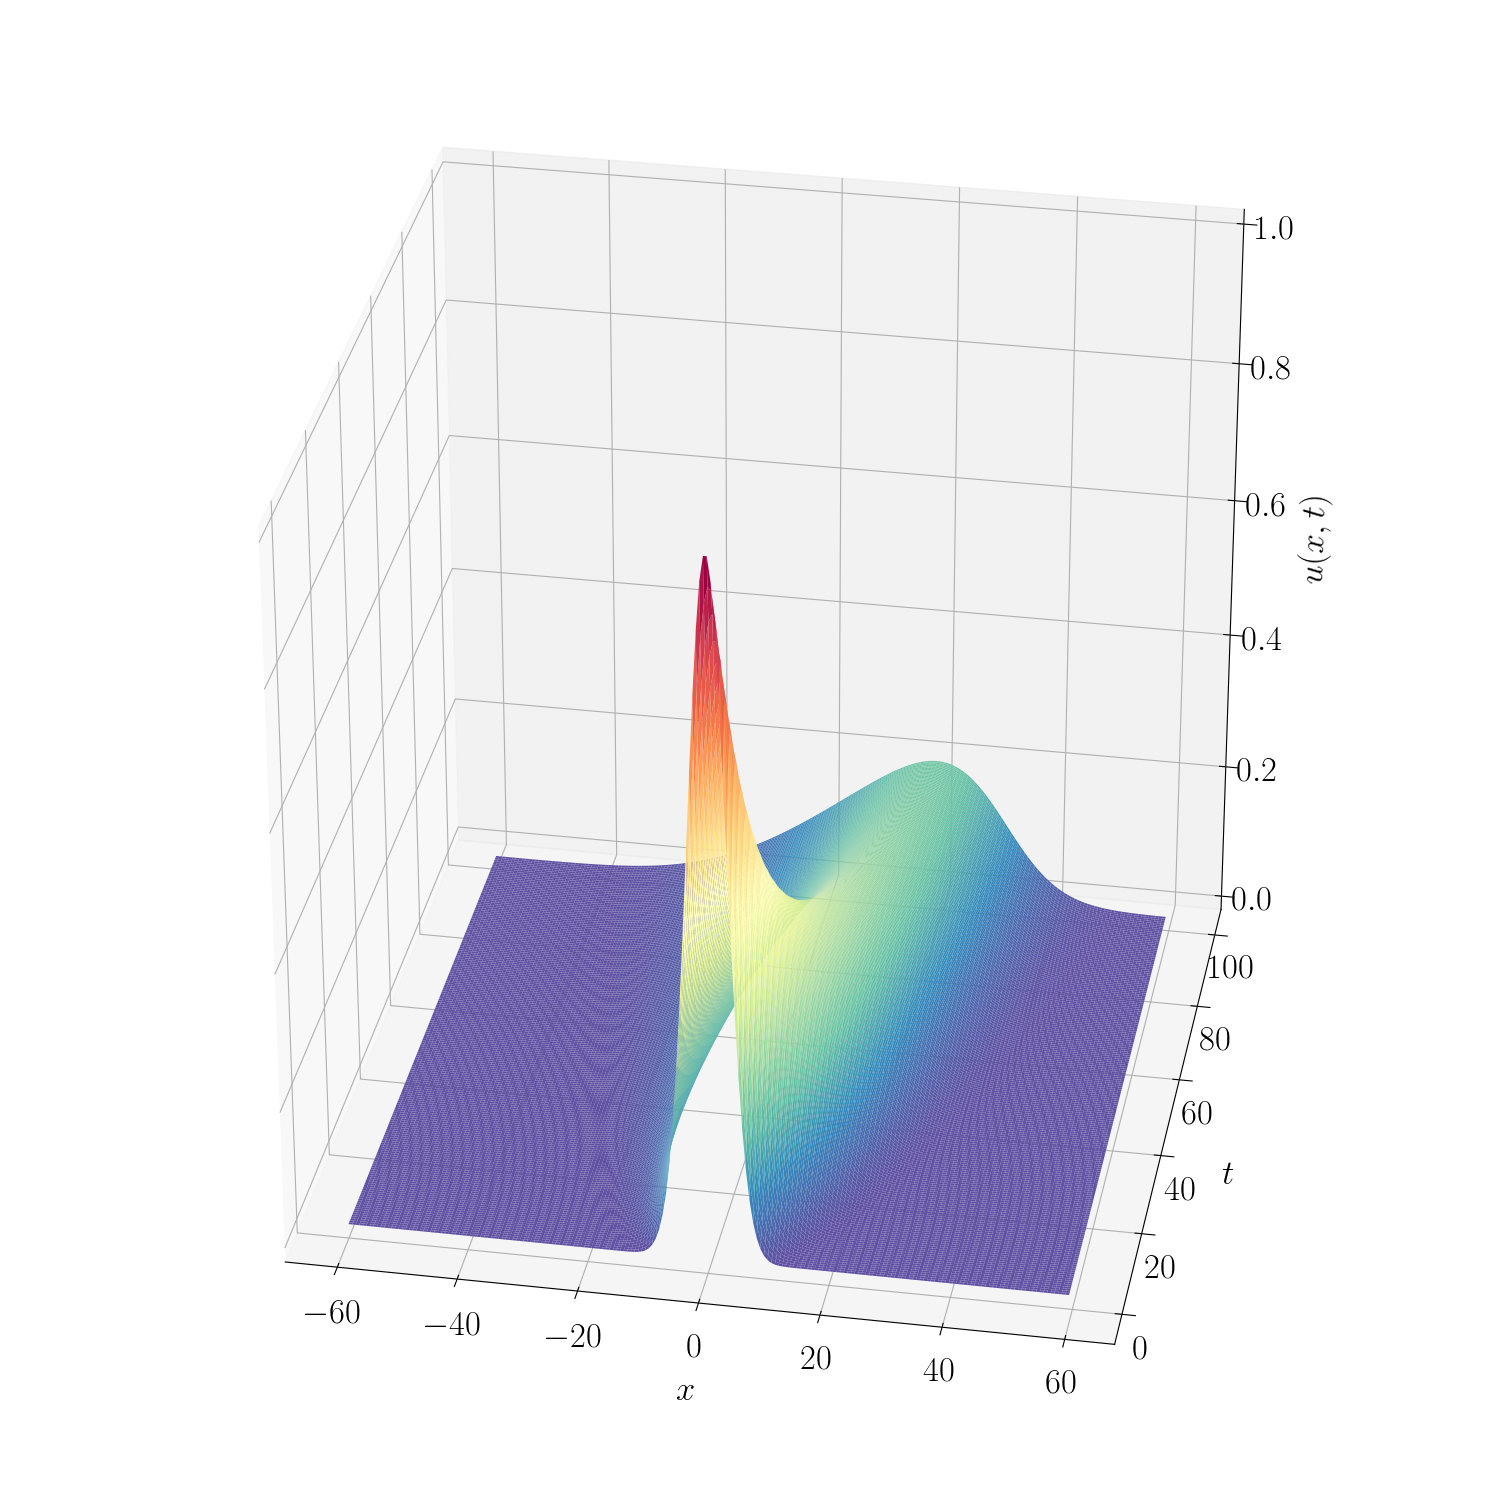
\includegraphics[width=12cm]{burgers_equation/deterministic/numerical_experiments/viscid/figures/galerkin/Numerical_Solution_alpha=1.png}
		\label{Galerkin_alpha=1}
		\caption{Numerical solution for (\ref{IVP_Burgers}) using (\ref{Galerkin_Euler}) at the time $T = 100$ with $\alpha = 1.0$, and $\Delta t = 1.0 \times 10^{-5}$. (b) Point-wise error of approximation}
		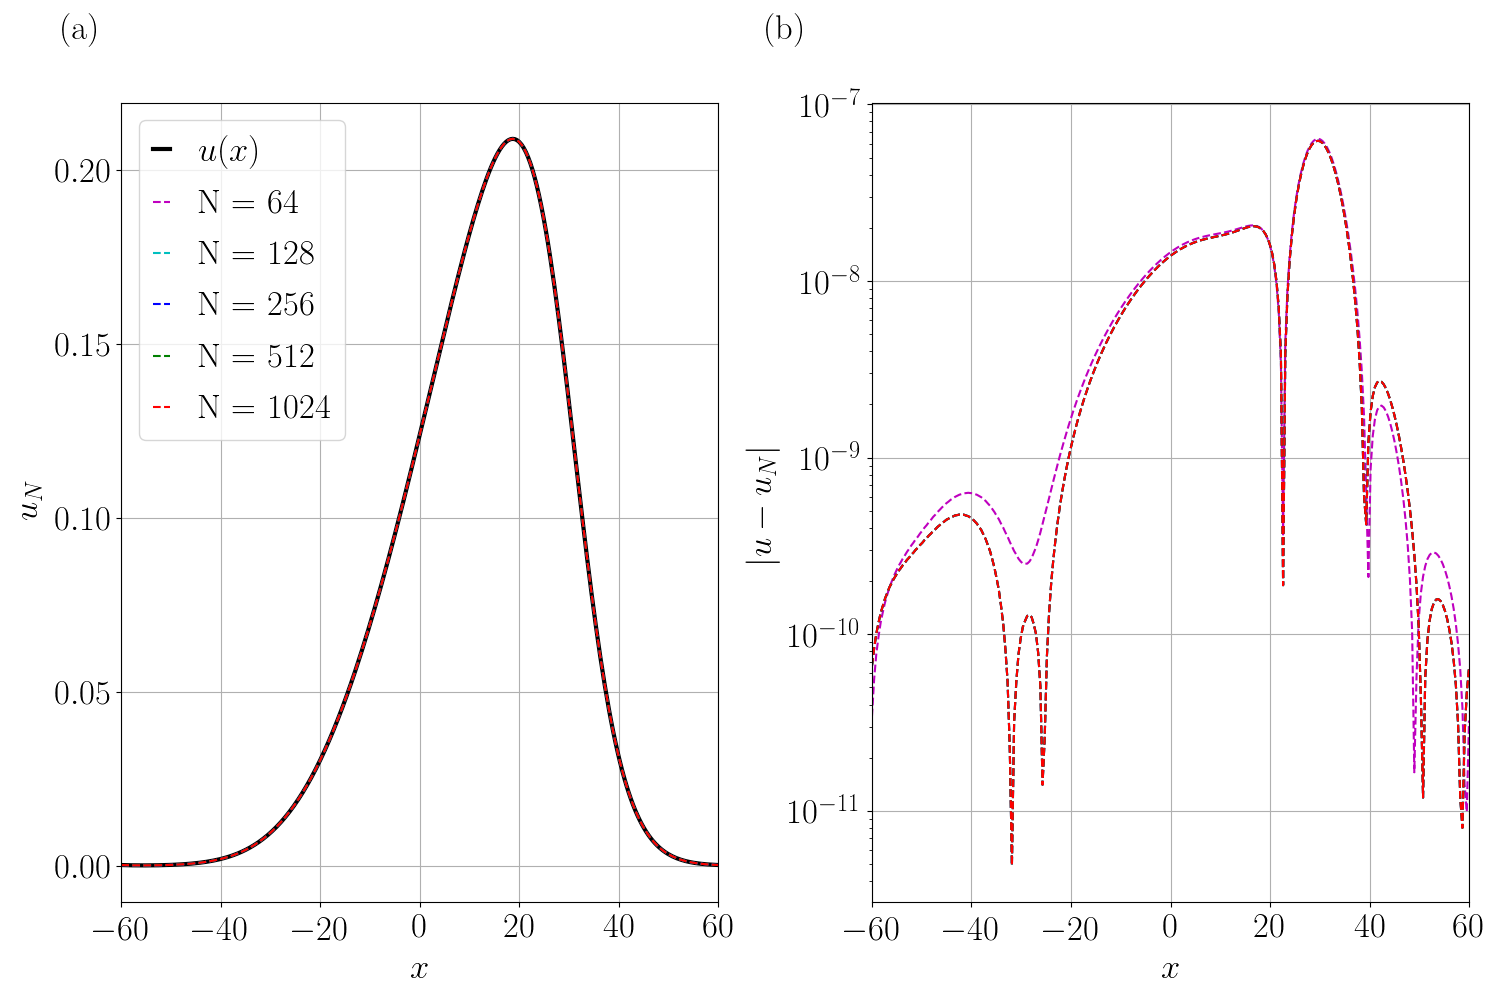
\includegraphics[width=12.5cm]{burgers_equation/deterministic/numerical_experiments/viscid/figures/galerkin/Numerical_Solution_alpha=1_T=100.png}
		\label{Galerkin_alpha=1_T}
	\end{figure}
	\begin{table}[H]
		\begin{tabular}{lcccc}
			\toprule
			\multicolumn{1}{c}{\textbf{Expansion}} & \multicolumn{4}{c}{\textbf{Error}} \\
			$\hspace{9mm}N$ & $\Delta t=1\times 10^{-2}$ & $\Delta t=1\times 10^{-3}$ & $\Delta t=1\times 10^{-4}$ & $\Delta t=1\times 10^{-5}$ \\
			\midrule
			\hspace{7mm} 16 & 0.72504    & 0.72504    & 0.72504    & 0.72504    \\
			\midrule
			\hspace{7mm} 32 & 6.90249 $\times 10 ^{-2}$   & 6.88052 $\times 10 ^{-2}$   & 6.87838 $\times 10 ^{-2}$   & 6.87816 $\times 10 ^{-2}$   \\
			\midrule
			\hspace{7mm} 64 & 1.23827 $\times 10 ^{-3}$  & 8.85367 $\times 10 ^{-4}$ & 8.80521 $\times 10 ^{-4}$ & 8.80410 $\times 10 ^{-4}$  \\
			\midrule
			\hspace{7mm} 128 & 9.43454 $\times 10 ^{-4}$ & 9.41793 $\times 10 ^{-5}$ & 9.41148 $\times 10 ^{-6}$ & 9.41827 $\times 10 ^{-7}$  \\
			\midrule
			\hspace{7mm} 256 & 9.43454 $\times 10 ^{-4}$ & 9.41793 $\times 10 ^{-5}$ & 9.41109 $\times 10 ^{-6}$ & 9.36411 $\times 10 ^{-7}$ \\
			\midrule
			\hspace{7mm} 512 & 9.43454 $\times 10 ^{-4}$ & 9.41793 $\times 10 ^{-5}$ & 9.41109 $\times 10 ^{-6}$ & 9.36411 $\times 10 ^{-7}$ \\
			\midrule
			\hspace{7mm} 1024 & $\ast$ & 9.41793 $\times 10^{-5}$ & 9.41109 $\times 10^{-6}$ & 9.36411 $\times 10^{-7}$              \\
			\midrule
			\hspace{7mm} 2048 & $\ast$ & $\ast$ & 9.41109 $\times 10^{-6}$ & 9.36411 $\times 10^{-7}$   \\
			\bottomrule
		\end{tabular}
		\caption{Error using $L^2$-norm with $\alpha = 1.0$}
		\label{Galerkin_tabla_L2_alpha=1}
		\vspace{1cm}
		\begin{tabular}{lcccc}
			\toprule
			\multicolumn{1}{c}{\textbf{Expansion}} & \multicolumn{4}{c}{\textbf{Error}} \\
			$\hspace{9mm}N$ & $\Delta t=1\times 10^{-2}$ & $\Delta t=1\times 10^{-3}$ & $\Delta t=1\times 10^{-4}$ & $\Delta t=1\times 10^{-5}$ \\
			\midrule
			\hspace{7mm} 16 & 0.203363    & 0.203333    & 0.203331    & 0.20333     \\
			\midrule
			\hspace{7mm} 32 & 2.64192 $\times 10 ^{-2}$   & 2.6248 $\times 10 ^{-2}$    & 2.62491 $\times 10 ^{-2}$  & 2.62492 $\times 10 ^{-2}$   \\
			\midrule
			\hspace{7mm} 64 & 6.93001 $\times 10 ^{-4}$ & 4.11641 $\times 10 ^{-4}$ & 3.85563 $\times 10 ^{-4}$ & 3.82972 $\times 10 ^{-4}$ \\
			\midrule
			\hspace{7mm} 128 & 4.74934 $\times 10 ^{-4}$ & 4.73649 $\times 10 ^{-5}$ & 4.74295 $\times 10 ^{-6}$ & 5.16105 $\times 10 ^{-7}$ \\
			\midrule
			\hspace{7mm} 256 & 4.74936 $\times 10 ^{-4}$ & 4.7368 $\times 10 ^{-5}$  & 4.72569 $\times 10 ^{-6}$ & 4.64922 $\times 10 ^{-7}$ \\
			\midrule
			\hspace{7mm} 512 & 4.74936 $\times 10 ^{-4}$ & 4.7368 $\times 10 ^{-5}$  & 4.72569 $\times 10 ^{-6}$ & 4.64922 $\times 10 ^{-4}$ \\
			\midrule
			\hspace{7mm} 1024 & * & 4.7368 $\times 10 ^{-5}$  & 4.72569 $\times 10 ^{-6}$ & 4.64922 $\times 10 ^{-7}$ \\
			\midrule
			\hspace{7mm} 2048 & * & * & 4.72569 $\times 10 ^{-6}$ & 4.64922 $\times 10 ^{-7}$ \\
			\bottomrule
		\end{tabular}
		\caption{Error using Max norm with $\alpha = 1.0$}
		\label{Galerkin_tabla_max_alpha=1}
	\end{table}

	\begin{figure}[H]
		\centering
		\caption{Numerical solution for (\ref{IVP_Burgers}) using (\ref{Galerkin_Euler}) with $\alpha = 0.005$, $N=2048$, and $\Delta t = 1.0 \times 10^{-5}$.}
		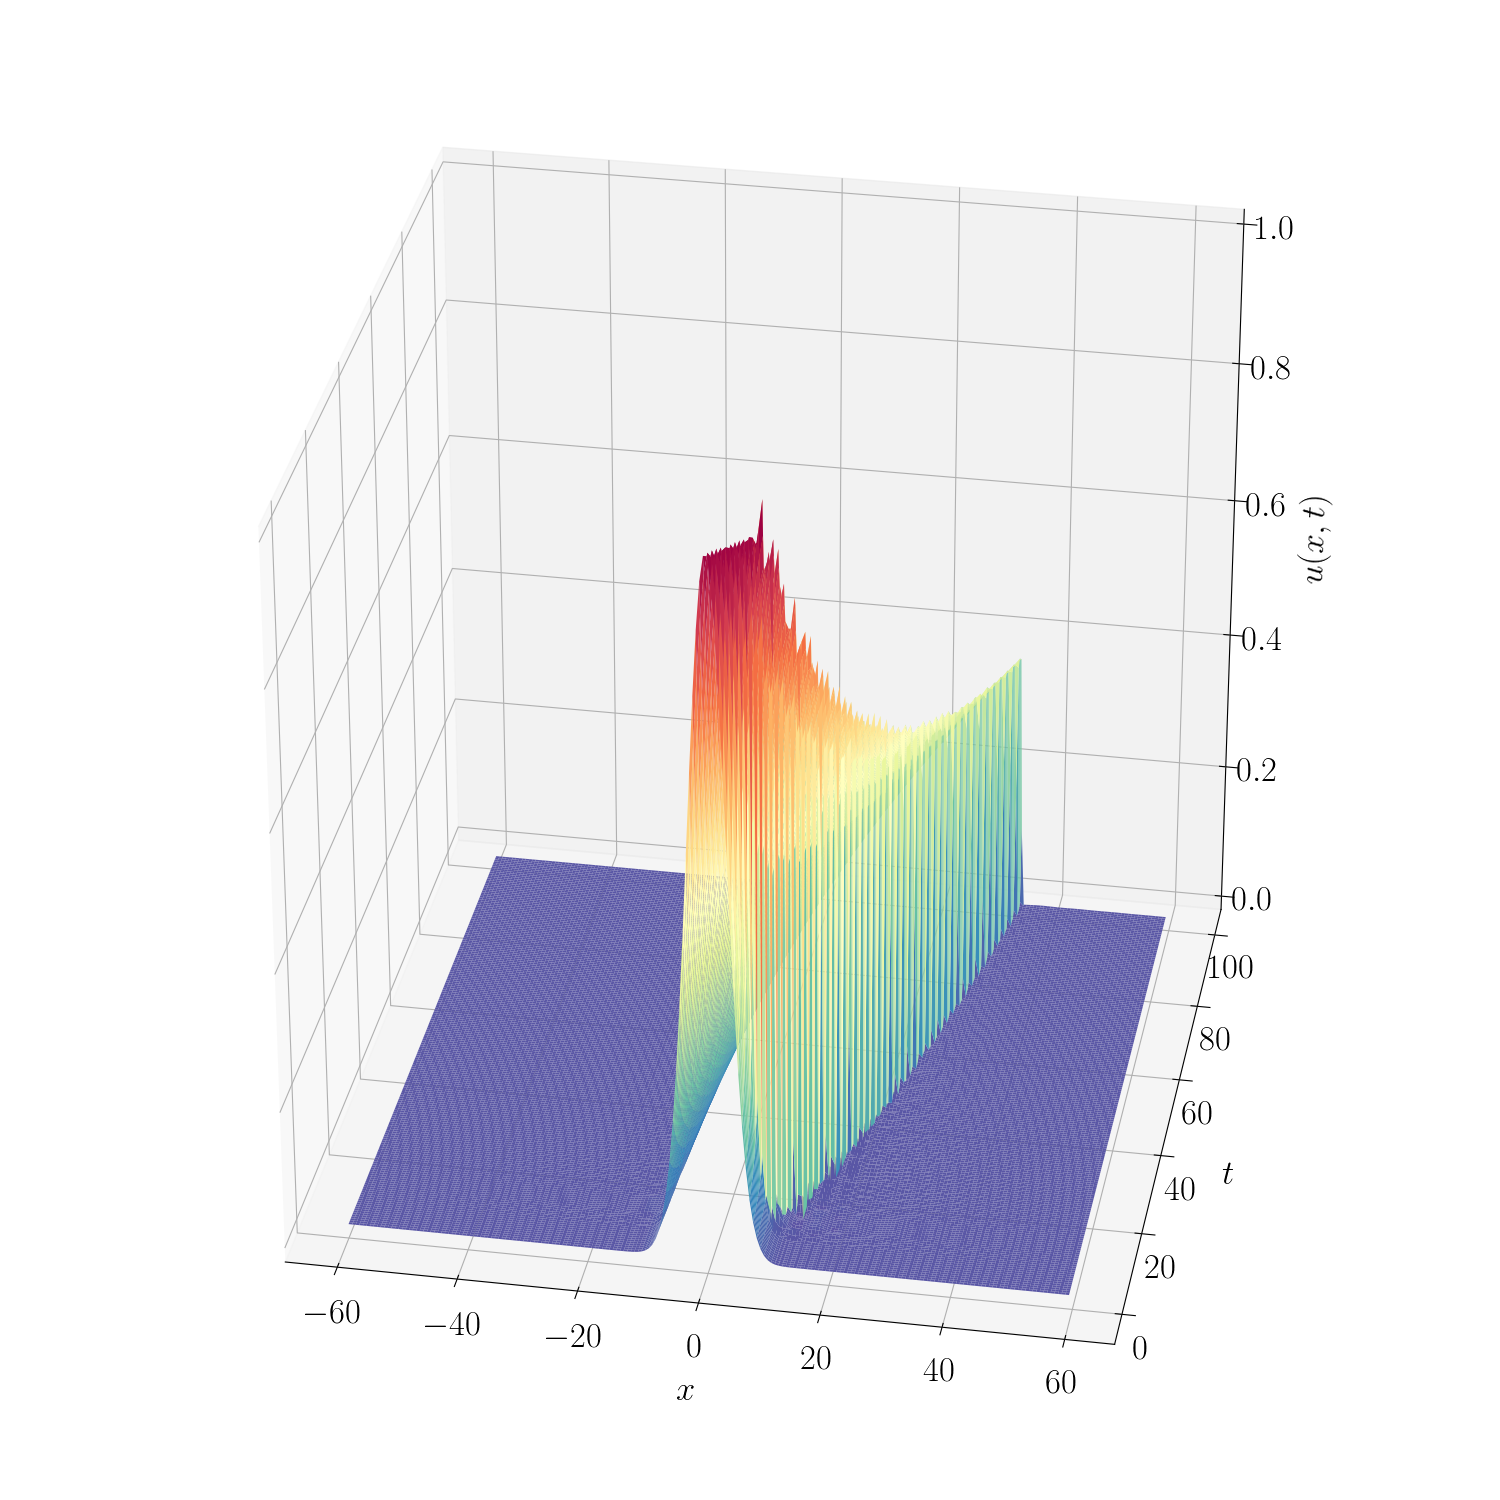
\includegraphics[width=12cm]{burgers_equation/deterministic/numerical_experiments/viscid/figures/galerkin/Numerical_Solution_alpha=0005.png}
		\caption{Numerical solution for (\ref{IVP_Burgers}) using (\ref{Galerkin_Euler}) at the time $T = 100$ with $\alpha = 1.0$, and $\Delta t = 1.0 \times 10^{-5}$. (b) Point-wise error of approximation}
		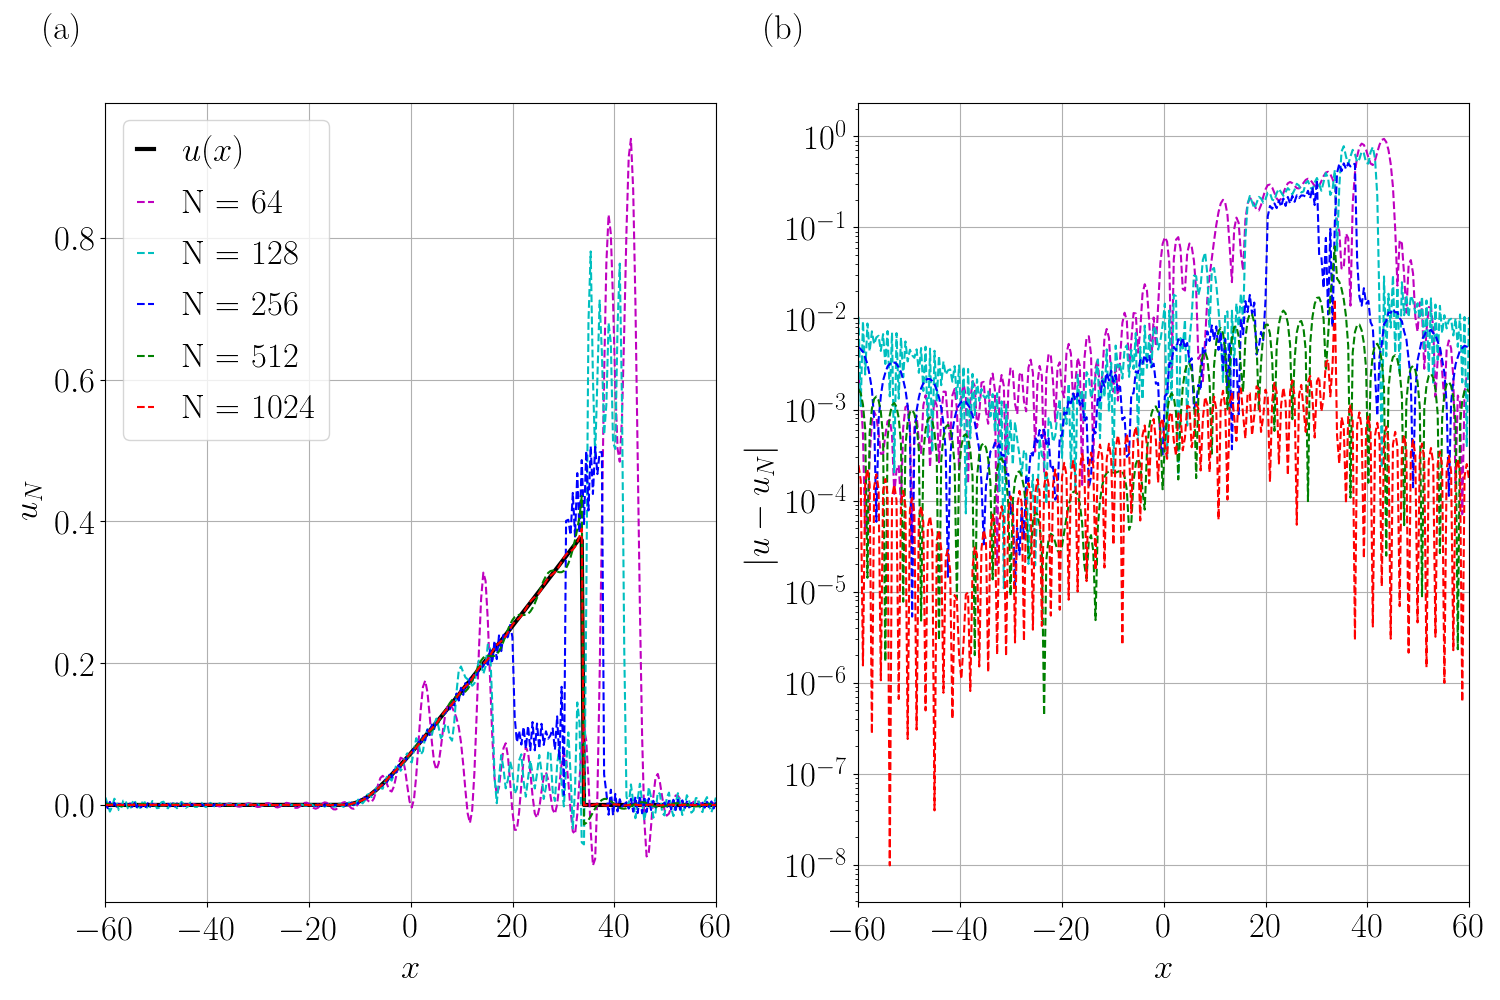
\includegraphics[width=12.5cm]{burgers_equation/deterministic/numerical_experiments/viscid/figures/galerkin/Numerical_Solution_alpha=0005_T=100.png}
		\label{Galerkin_alpha=005_T}
	\end{figure}
	
	\begin{table}[H]
	\begin{tabular}{lcccc}
		\toprule
		\multicolumn{1}{c}{\textbf{Expansion}} & \multicolumn{4}{c}{\textbf{Error}} \\
		$\hspace{9mm}N$ & $\Delta t=1\times 10^{-2}$ & $\Delta t=1\times 10^{-3}$ & $\Delta t=1\times 10^{-4}$ & $\Delta t=1\times 10^{-5}$ \\
		\midrule
		\hspace{7mm} 16 & 9.95328   & 9.91901    & 9.91597    & 9.91567    \\
		\midrule
		\hspace{7mm} 32 & 2.72607   & 2.70558    & 2.70347    & 2.70326    \\
		\midrule
		\hspace{7mm} 64 & 2.50343   & 2.45988    & 2.45543    & 2.45497    \\
		\midrule
		\hspace{7mm} 128 & 2.16142   & 2.06992    & 2.05918    & 2.05795    \\
		\midrule
		\hspace{7mm} 256 & 1.3658    & 1.19385    & 1.17602    & 1.17412    \\
		\midrule
		\hspace{7mm} 512 & 0.339826  & 0.265843   & 0.262164   & 0.261805   \\
		\midrule
		\hspace{7mm} 1024 & 0.161405  & 0.133743   & 0.131882   & 0.131699   \\
		\midrule
		\hspace{7mm} 2048 & 6.50292 $\times 10^{-2}$ & 4.70602 $\times 10^{-2}$ & 4.57371 $\times 10^{-2}$  & 4.56090 $\times 10^{-2}$  \\
		\bottomrule
	\end{tabular}
	\caption{Error using $L^2$-norm with $\alpha = 0.005$}
	\label{Galerkin_tabla_L2_alpha=005}
	\vspace{1cm}
	\begin{tabular}{lcccc}
		\toprule
		\multicolumn{1}{c}{\textbf{Expansion}} & \multicolumn{4}{c}{\textbf{Error}} \\
		$\hspace{9mm}N$ & $\Delta t=1\times 10^{-2}$ & $\Delta t=1\times 10^{-3}$ & $\Delta t=1\times 10^{-4}$ & $\Delta t=1\times 10^{-5}$ \\
		\midrule
		\hspace{7mm} 16 & 2.50002  & 2.48992   & 2.48891   & 2.48881   \\
		\midrule
		\hspace{7mm} 32 & 1.21263  & 1.20544   & 1.2047    & 1.20463   \\
		\midrule
		\hspace{7mm} 64 & 1.21269  & 1.17736   & 1.17517   & 1.17495   \\
		\midrule
		\hspace{7mm} 128 & 1.10164  & 1.03493   & 1.03093   & 1.03048   \\
		\midrule
		\hspace{7mm} 256 & 0.954369 & 0.881472  & 0.873392  & 0.87259   \\
		\midrule
		\hspace{7mm} 512 & 0.665071 & 0.418735  & 0.398664  & 0.396931  \\
		\midrule
		\hspace{7mm} 1024 & 0.241841 & 0.244188  & 0.244437  & 0.244461  \\
		\midrule
		\hspace{7mm} 2048 & 0.133067 & 0.104675  & 0.109151  & 0.109596  \\
		\bottomrule
	\end{tabular}
	\caption{Error using Max norm with $\alpha =0.005$}
	\label{Galerkin_tabla_max_alpha=005}
	\end{table}
	
	\newpage

	\subsubsection{Simulations for Fourier-Collocation Method}
	
	Following the same ideas from the previous section for Fourier-Collocation, we will seek solutions in the space given by $S_N = \widetilde{B}_N \cap H^2_p [0, 2 \pi]$, and using the discrete expansion to the problem (\ref{IVP_Burgers}) as follows
	\begin{align*}
		\mathcal{J}_N u (x, t) =  \displaystyle \sum_{|n| \leq \frac{N}{2}} \widetilde{u}_n (t) e^{inx}, \hspace{2mm}
		\widetilde{u}_n (t) =  \displaystyle \sum_{j=0}^{2N} u (x_j, t)  e^{-in x_j}
	\end{align*}
	or equivalently
	\begin{align*}
		\mathcal{J}_N u (x, t) =  \displaystyle \sum_{j=0}^{2N} u (x_j, t) \psi_j (x)
	\end{align*} 
	where $x_j$ are given by
	\begin{align*}
		xj = \frac{2 \pi j}{2N + 1}, \hspace{2mm} j = 0, 1, \dots, 2N.
	\end{align*}
	
	For this case, the Fourier-Collocation method will be given by the following problem
	\begin{align}
	\label{Collocation_Nonlinear}	
		R_{N} (x_j, t) = \frac{\partial u_N}{\partial t} (x_j, t) - \frac{\partial^2 u_N }{\partial x^2} (x_j, t) + \frac{1}{2} \frac{\partial \left[ u_N \right]^2}{\partial x} (x_j, t) = 0
	\end{align}
	which is a system of $2N + 1$ ordinary differential equations that can be solved using the initial condition given by
	\begin{align*}
		\mathcal{J}_N u (x_j, t) =  u_0 (x_j), , \hspace{2mm} j = 0, 1 \dots, 2N
	\end{align*}
	
	By Setting a vector as follows
	\begin{align*}
		u_N (t) &= (u_N (x_0 , t), u_N (x_1 , t), \dots , u_N (x_{2N} , t))^T,
	\end{align*} 
	and the above system of ordinary differential equations can be written as follows
	\begin{align*}
		\frac{d u_N (t)}{dt} =  \alpha D_N^2 u_N (t) - \frac{1}{2} D_N u^2_N (t)
	\end{align*}
	where $D_N$ is the matrix given by (\ref{matrix_DN_odd}), that represents discrete Fourier differentiation, which can be rewrite as
	\begin{align}
		D_N = \displaystyle C^{-1} \Lambda^2_N C
	\end{align}
	where $\Lambda_N = diag \{ ik \}_{|k|\leq N}$, $C$ represents the discrete Fourier transform and $C^{-1}$ the inverse. \\
	
	Note that the situation here is very different compared to the systems obtained with Fourier-Galerkin. The representation of the non-linear term is more practical to handle with implicit methods, for example, an implicit approach is as follows
	\begin{align*}
		u_N (t_{i + 1} ) =  C^{-1} \Lambda_N C u_N (t_{i}) - \frac{\Delta t}{2} D_N u^2_N (t_{i+1}) 
	\end{align*}
	
	It is possible to formulate the above problem as 
	\begin{align*}
		W(u_N (t_{i + 1})) =  C^{-1} \Lambda_N C u_N (t_{i}) - u_N (t_{i + 1} ) - \frac{\Delta t}{2} D_N u^2_N (t_{i+1}), 
	\end{align*}
	and then we must find $u_N(t_{i + 1})$ that satisfies $W(u_N(t_{i + 1})) = 0$, for example, using the Newton-Raphson method. However, this formulation may require many calculations because the differentiation matrix increases as a function of $N$, and therefore the number of operations. Here we are going to develop a numerical solution that is more practical to implement, implicitly approaching as we did with Fourier-Galerkin on the linear term as follows
	\begin{align*}
		\left[I_N + \frac{\Delta t}{2} u_{0} \Lambda_N \right] u_N (t_{i + 1} ) =  \displaystyle e^{-\Delta t \Lambda^0_N} \left[ u_N (t_{i}) - \frac{\Delta t}{2} D_N u^2_N (t_{i}) \right]
	\end{align*}
	where $\Lambda^0_N = diag \{ \alpha k^2 + \frac{ik}{2} u_0 \}_{|k|\leq N}$, and solving for $u_N (t_{i + 1})$ gives us
	\begin{align}
	\label{Collocation_Euler}	
		u_N (t_{i + 1} ) =  \displaystyle \left[I_N + \frac{\Delta t}{2} u_{0} \Lambda_N \right]^{-1} e^{-\Delta t \Lambda^0_N} \left[ u_N (t_{i})  - \frac{\Delta t}{2} D_N u^2_N (t_{i}) \right]
	\end{align}
	which is very similar to \ref{Galerkin_Euler}, except for the nonlinear term. \\
	  
	This formulation will be used for its implementation, and we will present some numerical results that were obtained using the same information that was used with Fourier-Galerkin, the difference is that the calculations are performed in real space using the differentiation matrix $D_N$, and in this case, we have the advantage of approximating the second derivative with $D^2_N = D_N \cdot D_N$. \\
	
	The description of the following results is as follows. In the figure \ref{Collocation_alphas} shows the maximum distance over every $t \in [0, 100]$ between the exact solution and its approximations given by (\ref{Collocation_Euler}) for $N = 2^m$, $m = 4, \dots, 12$, $\Delta t = 1.0 \times 10^{-5}$, and different values of $\alpha$. Furthermore, in Tables \ref{Collocation_tabla_L2_alpha=1} and \ref{Collocation_tabla_max_alpha=1}, we can see the numerical values ​​of these distances for different configurations of $N$ and $\Delta t$. Similarly, in Tables \ref{Collocation_tabla_L2_alpha=005} and \ref{Collocation_tabla_max_alpha=005} but for $\alpha = 0.005$.
	
	\newpage
	\begin{figure}[H]
		\centering
		\includegraphics[width=12cm]{burgers_equation/deterministic/numerical_experiments/viscid/figures/collocation/alphas_Error_N.png}
		\caption{(a) $L^2$-norm between the exact solution and its approximations using Collocation method. (b) Max norm between the exact solution and its approximations.}
		\label{Collocation_alphas}
	\end{figure}

	\newpage
	\begin{figure}[H]
		\centering
		\caption{Numerical solution for (\ref{IVP_Burgers}) using (\ref{Collocation_Euler}) with $\alpha = 1.0$, $N=2048$, and $\Delta t = 1.0 \times 10^{-5}$.}
		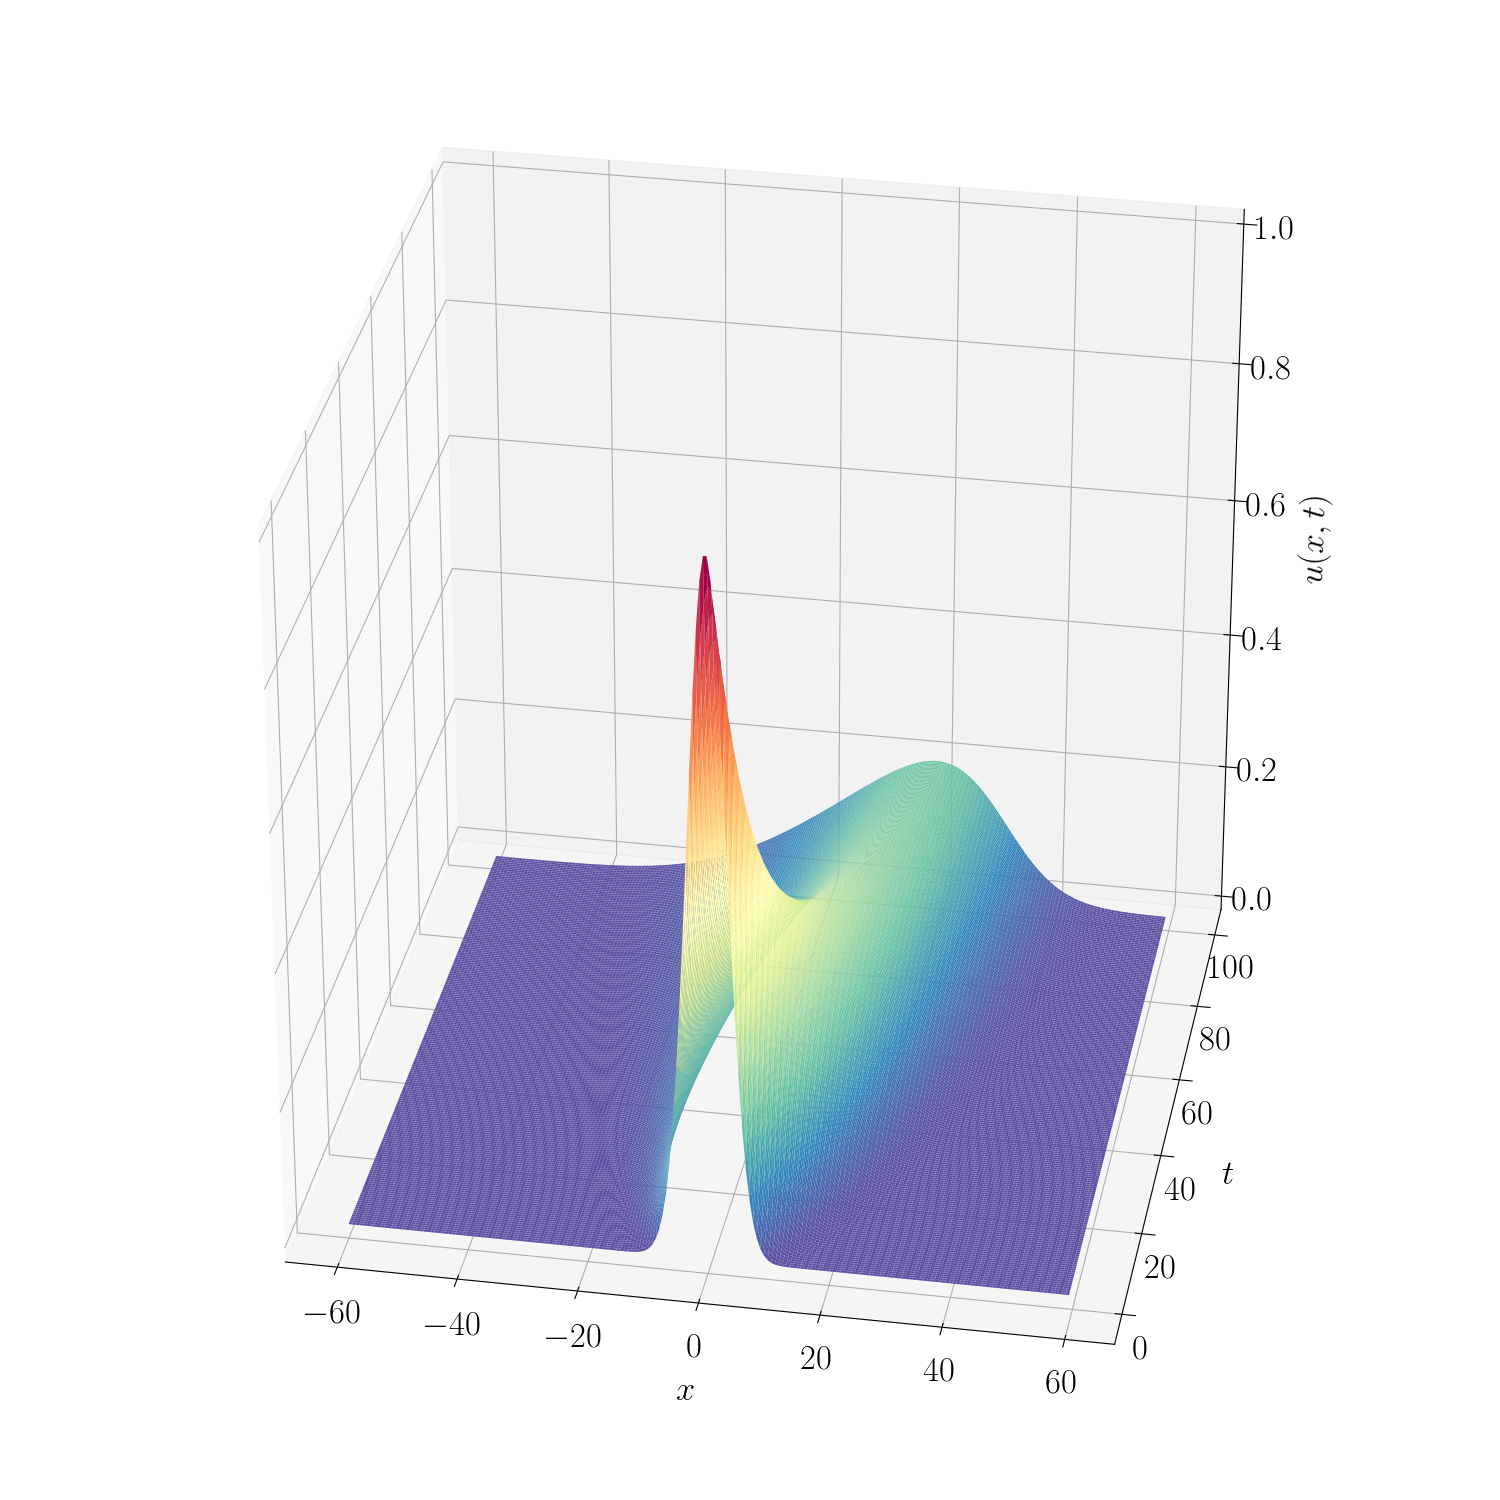
\includegraphics[width=12cm]{burgers_equation/deterministic/numerical_experiments/viscid/figures/collocation/Numerical_Solution_alpha=1.png}
		\label{Collocation_alpha=1}
		\caption{Numerical solution for (\ref{IVP_Burgers}) using (\ref{Collocation_Euler}) at the time $T = 100$ with $\alpha = 1.0$, and $\Delta t = 1.0 \times 10^{-5}$. (b) Point-wise error of approximation}
		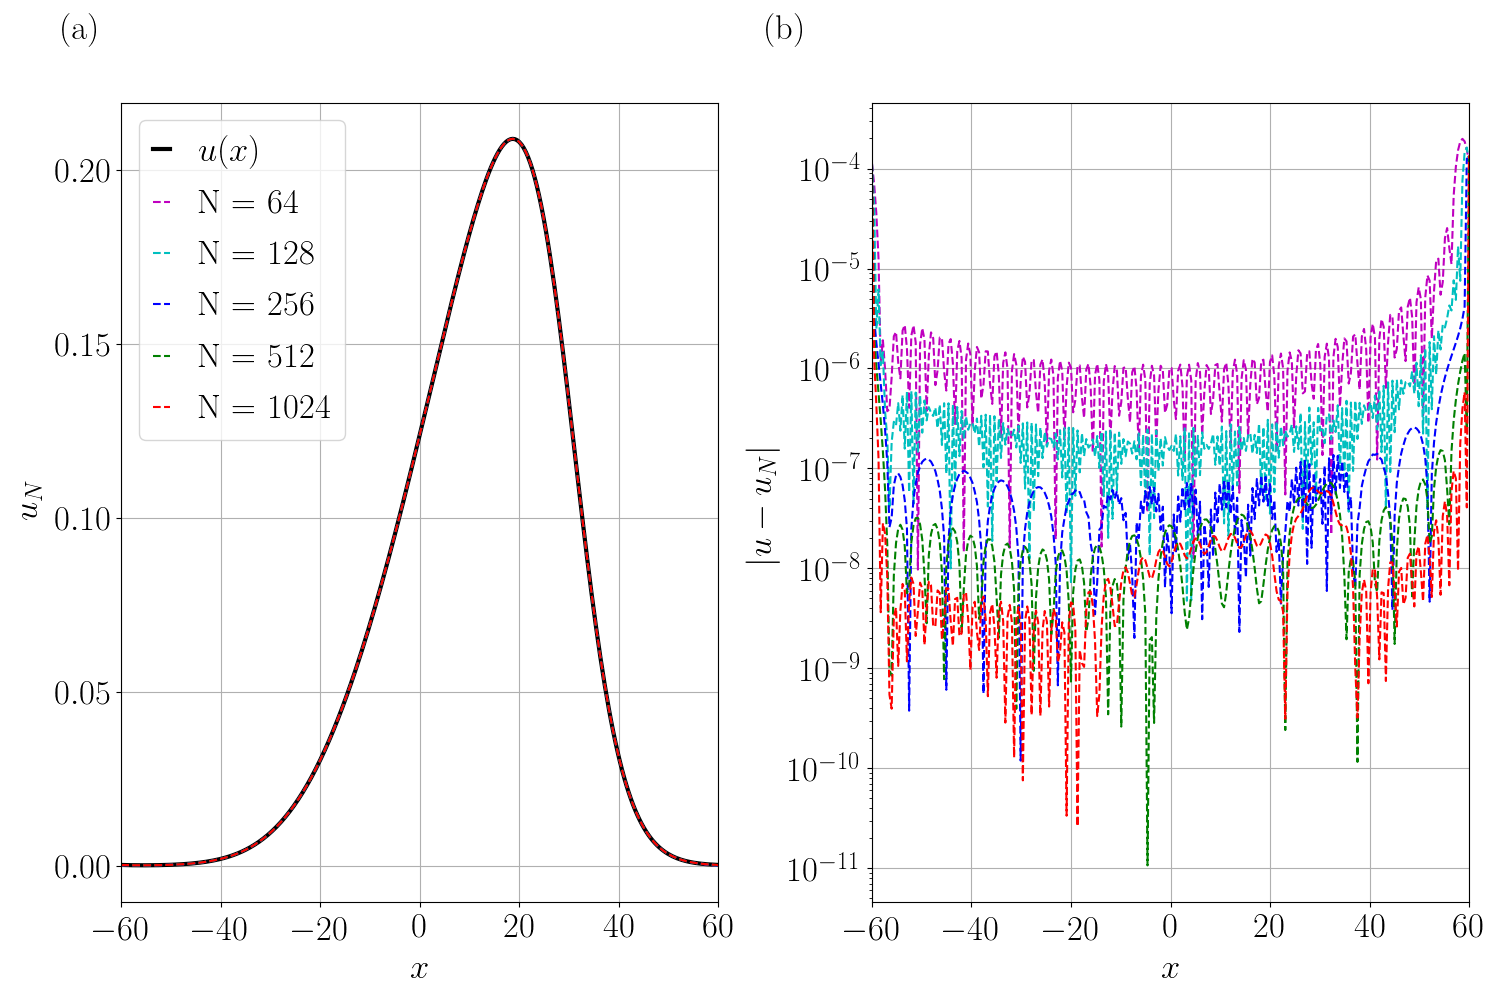
\includegraphics[width=12.5cm]{burgers_equation/deterministic/numerical_experiments/viscid/figures/collocation/Numerical_Solution_alpha=1_T=100.png}
		\label{Collocation_alpha=1_T}
	\end{figure}
	\begin{table}[H]
		\begin{tabular}{lcccc}
			\toprule
			\multicolumn{1}{c}{\textbf{Expansion}} & \multicolumn{4}{c}{\textbf{Error}} \\
			$\hspace{9mm}N$ & $\Delta t=1\times 10^{-2}$ & $\Delta t=1\times 10^{-3}$ & $\Delta t=1\times 10^{-4}$ & $\Delta t=1\times 10^{-5}$ \\
			\midrule
			\hspace{7mm} 16 & 0.721112    & 0.721112    & 0.721112    & 0.721112    \\
			\midrule
			\hspace{7mm} 32 & 4.71797 $\times 10^{-2}$   & 4.72892 $\times 10^{-2}$   & 4.73004 $\times 10^{-2}$   & 4.73015 $\times 10^{-2}$   \\
			\midrule
			\hspace{7mm} 64 & 1.17954 $\times 10^{-3}$  & 7.35344 $\times 10^{-4}$ & 7.27561 $\times 10^{-4}$ & 7.27283 $\times 10^{-4}$  \\
			\midrule
			\hspace{7mm} 128 & 9.43454 $\times 10^{-4}$ & 1.75152 $\times 10^{-4}$ & 1.74583 $\times 10^{-4}$ & 1.74574 $\times 10^{-4}$ \\
			\midrule
			\hspace{7mm} 256 & 9.43454 $\times 10^{-4}$ & 1.15509 $\times 10^{-4}$ & 1.14669 $\times 10^{-4}$ & 1.14659 $\times 10^{-4}$ \\
			\midrule
			\hspace{7mm} 512 & 9.43454 $\times 10^{-4}$ & 9.41793 $\times 10^{-5}$ & 7.78847 $\times 10^{-5}$ & 7.78707 $\times 10^{-5}$ \\
			\midrule
			\hspace{7mm} 1024 & $\ast$         & 9.41793 $\times 10^{-5}$ & 5.32213 $\times 10^{-5}$ & 5.32019 $\times 10^{-5}$ \\
			\midrule
			\hspace{7mm} 2048 & $\ast$           & $\ast$           & 3.56779 $\times 10^{-5}$ & 3.56498 $\times 10^{-5}$ \\
			\\
			\bottomrule
		\end{tabular}
		\caption{Error using $L^2$-norm with $\alpha=1.0$}
		\label{Collocation_tabla_L2_alpha=1}
		\vspace{1cm}
		\begin{tabular}{lcccc}
			\toprule
			\multicolumn{1}{c}{\textbf{Expansion}} & \multicolumn{4}{c}{\textbf{Error}} \\
			$\hspace{9mm}N$ & $\Delta t=1\times 10^{-2}$ & $\Delta t=1\times 10^{-3}$ & $\Delta t=1\times 10^{-4}$ & $\Delta t=1\times 10^{-5}$ \\
			\midrule
			\hspace{7mm} 16 & 0.317617    & 0.317617    & 0.317617    & 0.317617    \\
			\midrule
			\hspace{7mm} 32 & 1.95279 $\times 10 ^{-2}$  & 1.96812 $\times 10 ^{-2}$   & 1.96965 $\times 10 ^{-2}$   & 1.96981 $\times 10 ^{-2}$   \\
			\midrule
			\hspace{7mm} 64 & 6.21793 $\times 10 ^{-4}$ & 2.9813 $\times 10 ^{-4}$  & 2.80086 $\times 10 ^{-4}$ & 2.78934 $\times 10 ^{-4}$ \\
			\midrule
			\hspace{7mm} 128 & 4.74952 $\times 10 ^{-4}$ & 1.64746 $\times 10 ^{-4}$ & 1.6473 $\times 10 ^{-4}$  & 1.64728 $\times 10 ^{-4}$ \\
			\midrule
			\hspace{7mm} 256 & 4.74936 $\times 10 ^{-4}$ & 1.52482 $\times 10 ^{-4}$ & 1.52467 $\times 10 ^{-4}$ & 1.52465 $\times 10 ^{-4}$ \\
			\midrule
			\hspace{7mm} 512 & 4.74936 $\times 10 ^{-4}$ & 1.47249 $\times 10 ^{-4}$ & 1.47234 $\times 10 ^{-4}$ & 1.47232 $\times 10 ^{-4}$ \\
			\midrule
			\hspace{7mm} 1024 & $\ast$           & 1.45032 $\times 10 ^{-4}$ & 1.45017 $\times 10 ^{-4}$ & 1.45016 $\times 10 ^{-4}$ \\
			\midrule
			\hspace{7mm} 2048 & $\ast$           & $\ast$           & 1.43941 $\times 10 ^{-4}$ & 1.4394 $\times 10 ^{-4}$ \\
			\\
			\bottomrule
		\end{tabular}
		\caption{Error using Max norm with $\alpha=1.0$}
		\label{Collocation_tabla_max_alpha=1}
	\end{table}
	
	
	\begin{figure}[H]
		\centering
		\caption{Numerical solution for (\ref{IVP_Burgers}) using (\ref{Collocation_Euler}) with $\alpha = 0.005$, $N=2048$, and $\Delta t = 1.0 \times 10^{-5}$.}
		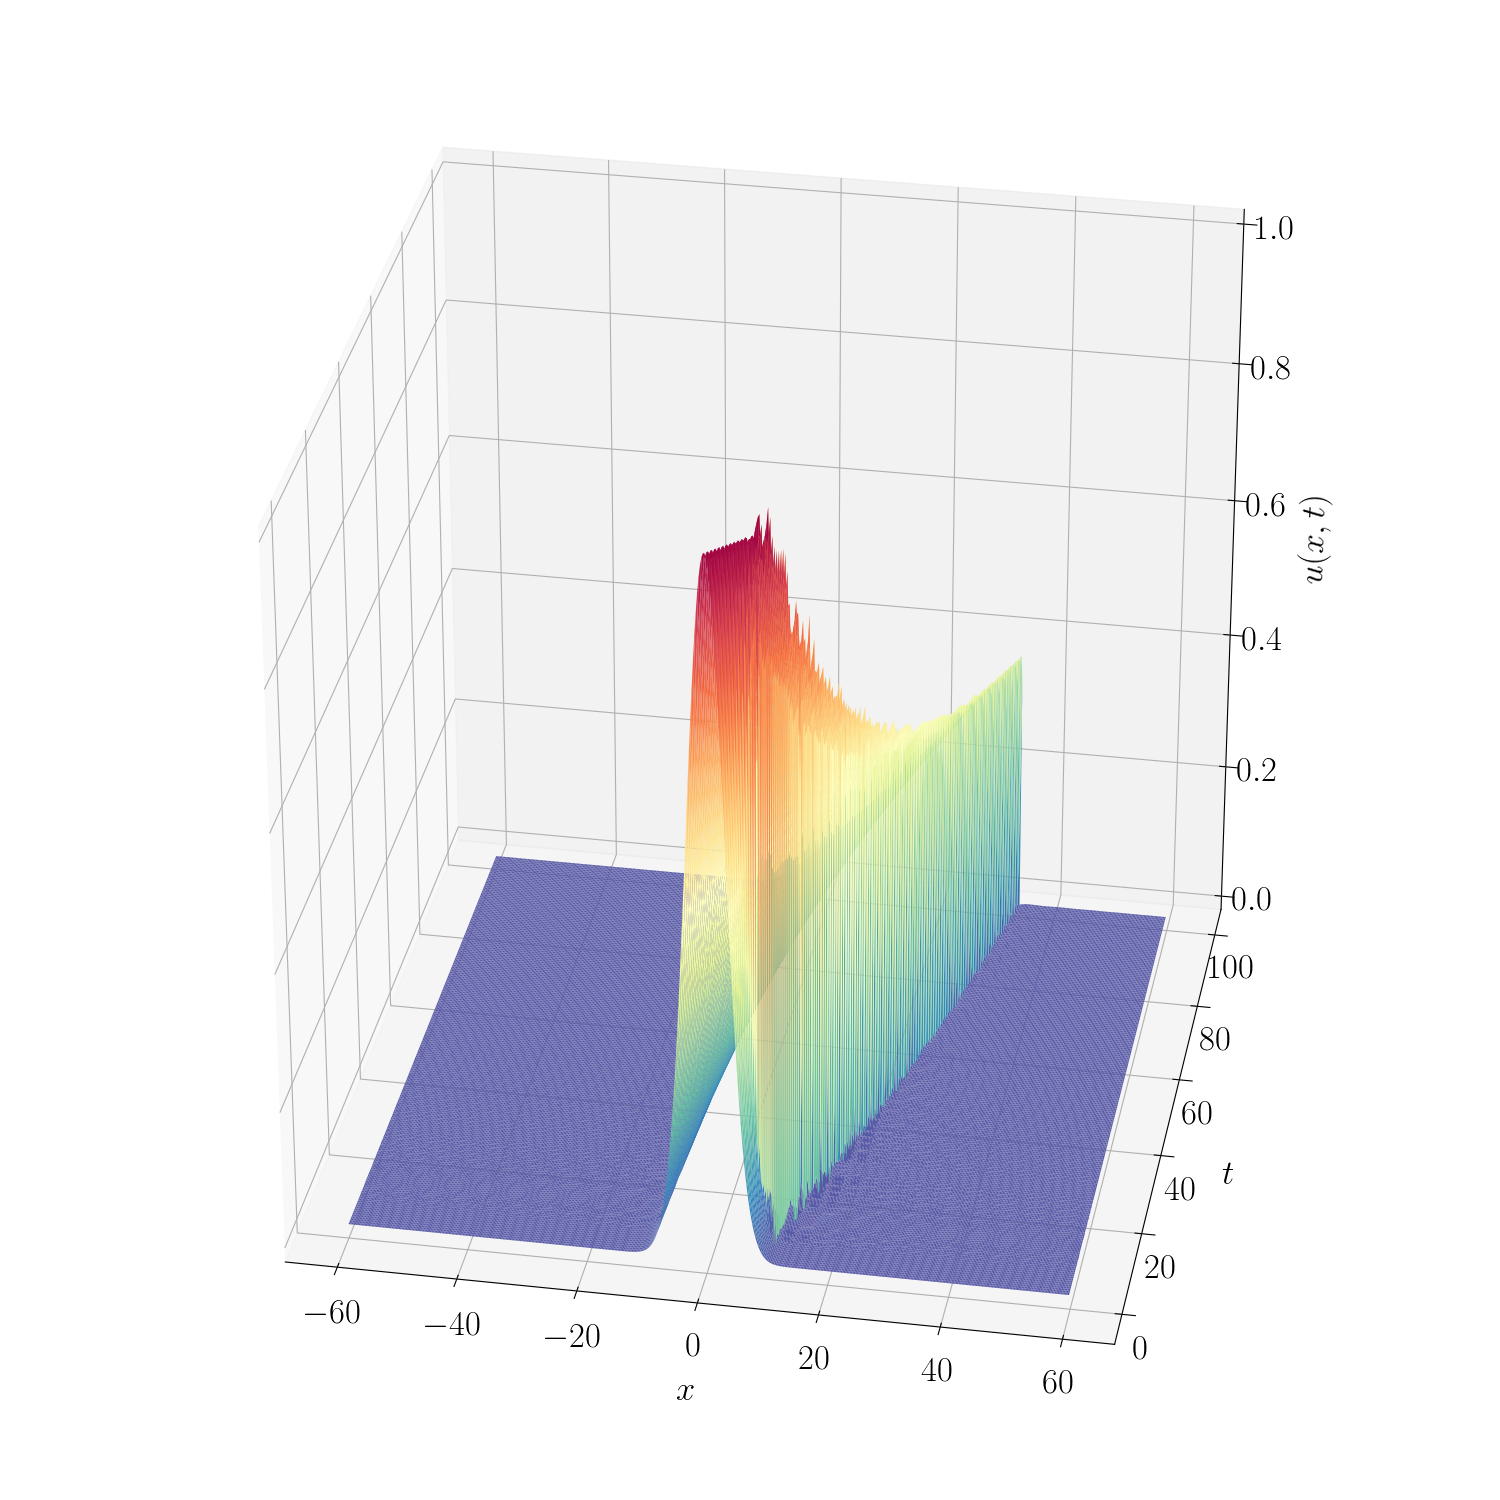
\includegraphics[width=12cm]{burgers_equation/deterministic/numerical_experiments/viscid/figures/collocation/Numerical_Solution_alpha=0005.png}
		\label{Collocation_alpha=005}
		\caption{Numerical solution for (\ref{IVP_Burgers}) using (\ref{Collocation_Euler}) at the time $T = 100$ with $\alpha = 0.005$, and $\Delta t = 1.0 \times 10^{-5}$. (b) Point-wise error of approximation.}
		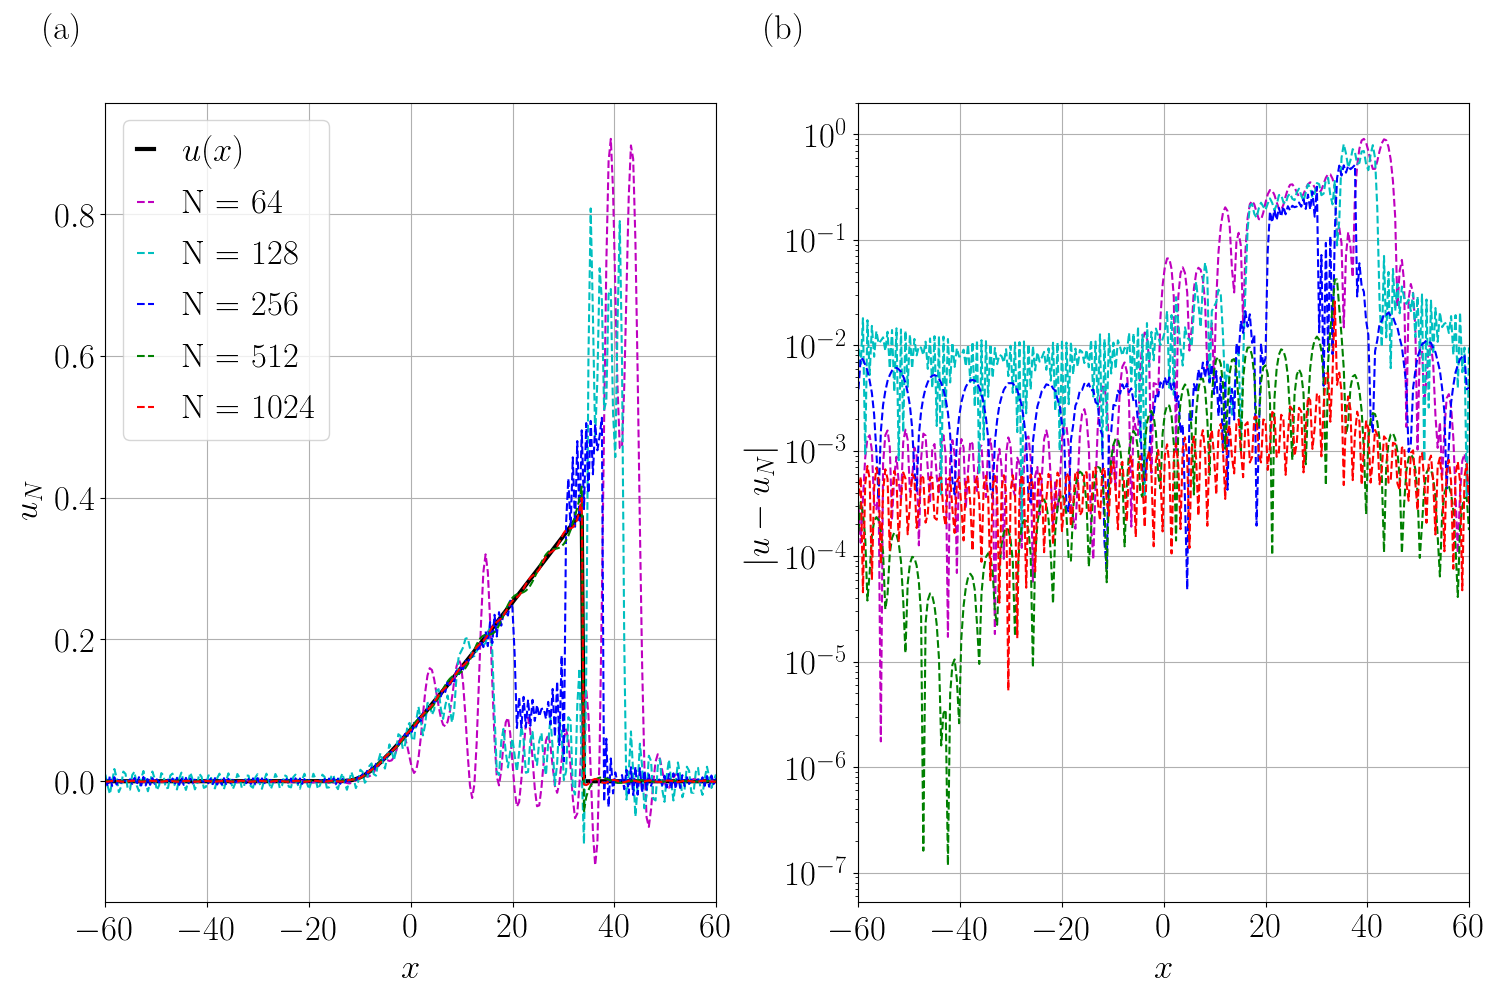
\includegraphics[width=12.5cm]{burgers_equation/deterministic/numerical_experiments/viscid/figures/collocation/Numerical_Solution_alpha=0005_T=100.png}
		\label{Collocation_alpha=005_T}
	\end{figure}
	%L2
	
	\begin{table}[H]
	\begin{tabular}{lcccc}
		\toprule
		\multicolumn{1}{c}{\textbf{Expansion}} & \multicolumn{4}{c}{\textbf{Error}} \\
		$\hspace{9mm}N$ & $\Delta t=1\times 10^{-2}$ & $\Delta t=1\times 10^{-3}$ & $\Delta t=1\times 10^{-4}$ & $\Delta t=1\times 10^{-5}$ \\
		\midrule
		\hspace{7mm} 16 & 1.36189   & 1.35883    & 1.35852   & 1.35849   \\
		\midrule
		\hspace{7mm} 32 & 2.67506   & 2.65305    & 2.65078   & 2.65055   \\
		\midrule
		\hspace{7mm} 64 & 2.50365   & 2.45855    & 2.45432   & 2.45387   \\
		\midrule
		\hspace{7mm} 128 & 2.15795   & 2.0632     & 2.05589   & 2.05497   \\
		\midrule
		\hspace{7mm} 256 & 1.362     & 1.18393    & 1.16697   & 1.16532   \\
		\midrule
		\hspace{7mm} 512 & 0.350775  & 0.304595   & 0.300865  & 0.300499  \\
		\midrule
		\hspace{7mm} 1024 & 0.168462  & 0.140332   & 0.13803   & 0.137804  \\
		\midrule
		\hspace{7mm} 2048 & 6.56161 $\times 10^{-2}$ & 4.63808 $\times 10^{-2}$  & 4.49226 $\times 10^{-2}$ & 4.47813 $\times 10^{-2}$ \\
		\\
		\bottomrule
	\end{tabular}
	\caption{Error using $L^2$-norm with $\alpha=0.005$}
	\label{Collocation_tabla_L2_alpha=005}
	\vspace{1cm}
	\begin{tabular}{lcccc}
		\toprule
		\multicolumn{1}{c}{\textbf{Expansion}} & \multicolumn{4}{c}{\textbf{Error}} \\
		$\hspace{9mm}N$ & $\Delta t=1\times 10^{-2}$ & $\Delta t=1\times 10^{-3}$ & $\Delta t=1\times 10^{-4}$ & $\Delta t=1\times 10^{-5}$ \\
		\midrule
		\hspace{7mm} 16 & 0.695784 & 0.695659  & 0.695646  & 0.695645 \\
		\midrule
		\hspace{7mm} 32 & 1.20278  & 1.19418   & 1.19329   & 1.1932   \\
		\midrule
		\hspace{7mm} 64 & 1.22454  & 1.18903   & 1.18507   & 1.18467  \\
		\midrule
		\hspace{7mm} 128 & 1.11999  & 1.0238    & 1.01754   & 1.01701  \\
		\midrule
		\hspace{7mm} 256 & 0.927954 & 0.877058  & 0.872508  & 0.87201  \\
		\midrule
		\hspace{7mm} 512 & 0.664133 & 0.415288  & 0.39714   & 0.395563 \\
		\midrule
		\hspace{7mm} 1024 & 0.247742 & 0.259451  & 0.260605  & 0.26072  \\
		\midrule
		\hspace{7mm} 2048 & 0.126824 & 0.103297  & 0.107102  & 0.10748  \\
		\\
		\bottomrule
	\end{tabular}
	\caption{Error using Max norm with $\alpha=0.005$}
	\label{Collocation_tabla_max_alpha=005}
	\end{table}
	\subsection{Numerical Solutions for Burgers' Equation without Viscosity}
	
	To finish the section, we will study the problem (\ref{IVP_Burgers}) without viscosity, that is, when $\alpha = 0$. So the problem is the following
	\begin{align}
	\label{IVP_Inviscid}
		\left \lbrace \begin{array}{ll}
			\frac{\partial u}{\partial t} + \frac{1}{2} (u^2)_x = 0, \hspace{2mm} 0 < t \leq T, \hspace{2mm} x \in \mathcal{D} \\
			\\
			u(x, 0) = u_0(x), \hspace{2mm} x \in \mathcal{D}
		\end{array}  \right .
	\end{align}

	This problem, which seems much simpler, turns out to be very interesting, because it presents relevant characteristics regarding the physical interpretation of the problem in general, that is, the case with non-zero viscosity. \\
	
	The previous equation interprets the conservation of energy and is considered as a non-linear conservation law. We can understand this if we consider the function $ u $ as the speed of a fluid that conserves its energy with a flow density given by $f(u) = \frac{u^2} {2}$. \\
	
	The above can be shown considering that $u \in H^1_p [\mathcal{D}]$, and multiplying by $u$ and integrating both sides of the equation on the domain $\mathcal{D}$ to prove that $\| u \|$ does not change over time, that is,
	\begin{align*}
		\frac{1}{2} \frac{d}{dt} \displaystyle \int_{0}^{2 \pi} u^2(x, t) dx = - \int_{0}^{2 \pi} u^2(x, t) \frac{\partial u(x, t)}{\partial x} dx = - \frac{1}{3} u^3(x, t) \Big|^{2 \pi}_{0}.
	\end{align*}
	and because $u$ is periodic, we have to
	\begin{align*}
		\frac{1}{2} \frac{d}{dt} \| u(x, t) \|^2 = 0.
	\end{align*}
	This means that the energy is conserved with the same initial energy since we must bear in mind that this represents the kinetic energy of a fluid that travels with a velocity given by $u_0$. \\
		
	In any problem, these characteristics are of utmost importance, this is because we must consider the behavior of the solutions when they must be approached with some numerical method. In the literature, when a solution remains bounded in time, the problem is said to be well defined. In the analysis context, this assures us the existence of a continuously differentiable solution $u$, and that besides being unique, it is possible to approximate it. \\
	
	However, approximating the solutions to this problem using spectral methods can be more complicated if its characteristics are not well understood. Next, we will see that under a certain condition it is possible to find a single analytical solution and that otherwise, it may lose its uniqueness when developing discontinuities. \\
			
	First, let's define the curves $x = x(t)$ that start at a point $x_0 \in \mathbb{R}$, and satisfy the following problem
	\begin{align*}
		\left \lbrace \begin{array}{ll}
			x' (t) = u(x(t), t), \hspace{2mm} t > 0, \\
			\\
			x(0) = x_0.
		\end{array} \right .  
	\end{align*}
	
	The solutions for each $x_0$ are known as characteristic curves, which pass through the solution $u = u (x (t), t)$. It is well known in the theory of differential equations that when $u(x, t)$ is locally Lipschitz in the variable $x$, and continues in the variable $t$, the above equation admits a single solution $x(t)$ for each $x_0 \in \mathbb{R}$. So, assuming the above we have that for a solution $ x (t) $ corresponding to a fixed $x_0 \in \mathbb{R}$, it satisfies the following
	\begin{align*}
		\frac{d}{dt} [u(x(t), t)] &= x' (t) u_x (x(t), t) + u_t (x(t), t) \\
		&= u(x(t), t) u_x (x(t), t) - u(x(t), t) u_x (x(t), t) = 0
	\end{align*}
	which tells us that the function $u(x (t), t)$ is independent of the variable $t$, remaining constant along the characteristic curve. Therefore, we have to
	\begin{align*}
		u(x(t), t) = u (x(0), 0) = u_0 (x_0)
	\end{align*}
	
	Furthermore, we have that the solution $ x (t) $ will be given by the following curve
	\begin{align*}
		x(t) = x_0 + u_0 (x_0) t, \hspace{2mm} t > 0.
	\end{align*}
	which allows us to write the solution $ u(x, t)$ as follows
	\begin{align}
	\label{Exact_Inviscid}	
		u(x, t) = u_0(x_0), \hspace{2mm} x_0 = x - u_0(x_0) t
	\end{align}
	
	Note that the Lipschitz condition is necessary for the uniqueness of the above solution, since, conversely, if we set two different starting points $x_0, x_1$ such that $x_0 <x_1$, then its curves characteristics intersect for some $t$, that is,
	\begin{align*}
		x_0 + u_0(x_0) t = x_1 + u_0 (x_1) t,
	\end{align*}
	and using the mean value theorem we have that for some $c \in (x_0, x_1)$ the time $t$ is given by
	\begin{align*}
		t = \frac{x_1 - x_0}{u_0 (x_0) - u_0 (x_1)} = - \frac{1}{u'_0(c)},
	\end{align*}
	
	The above tells us that when these two curves intersect, the solution $u (x, t)$ cannot be continuous in the time $ t $ given by the previous equation. This is because $u_0 (x_0) \neq u_0 (x_1)$, and since the solution is constant over time we would have that $u (x, t) = u_0 (x_0) = u_0 (x_1)$, which is impossible. \\
		
	Therefore, the time $t$ for which two curves intersect represents a discontinuity, and that can be calculated by
	\begin{align}
	\label{shock_time}	
			Tc = \min_{x \in \mathbb{R}} \left[  \frac{-1}{u'_0 (x)} \right]
	\end{align}
	and we can observe that the continuity of the solution $u$ is assured if $T_c < 0$, which depends only on the initial condition $u_0$. \\
	
	This type of information allows us to know the criteria that must be considered when implementing numerical methods, but also the physical interpretation of the problem can be useful. For example, the solution to this problem can be considered to simulate the evolution of the profile of a sea wave that deforms as it approaches the coast until it breaks. But when this occurs, the deformation of the wave stops precisely at the time $T_c$. \\
	
	We must consider that the problem without viscosity supposes that the fluid behaves in an ideal or perfect way, traveling as if they were separate sheets without rubbing. But in real life, fluids always have a certain degree of viscosity, that is, the fluid sheets can rub and cause energy dissipation, and for these cases, we could consider the problem with sufficiently small values ​​of $\alpha$. So a question that naturally arises is what the behavior of the solutions looks like when $\alpha$ approaches zero. \\
	
	In chapter \ref{Introduction} we obtained the solution of the problem (\ref{IVP_Burgers}), which is given by (\ref{Exact_Solution}), and from this equation we can see that the solutions are infinitely differentiable for any value of $\alpha> 0$. Instinctively, we can notice that the solution approaches the solution of the equation without viscosity when $\alpha$ approaches zero. In fact, the solution obtained as a limit when $\alpha$ approaches zero is known as the entropy solution, which has been studied in \cite{Tadmor1989}, \cite{Maday1989} and in \cite{Kruzkov1970} has been proved that this solution is unique. \\
	
	In order to illustrate what we have previously discussed, we will consider the problem (\ref{IVP_Inviscid}) with the following initial condition function
	\begin{align}
	\label{IC_Inviscid}	
		u_0 (x) = e^{-0.005x^2}, \hspace{3mm} x \in \mathcal{D}
	\end{align}
	where $\mathcal{D} = [x_L, x_R]$, and considering the interval $I = [0, T_c]$ for a value of $T_c$ given by (\ref{shock_time}). \\
	
	In the following simulations, we will use the Fourier-Galerkin method given in (\ref{Galerkin_Euler}) to obtain approximations with different values of $\alpha$, and we will see how they approximate the exact solution of the problem (\ref{IC_Inviscid} ) which was given in (\ref {Exact_Inviscid}).
	
	\newpage
	\begin{figure}[H]
		\centering
		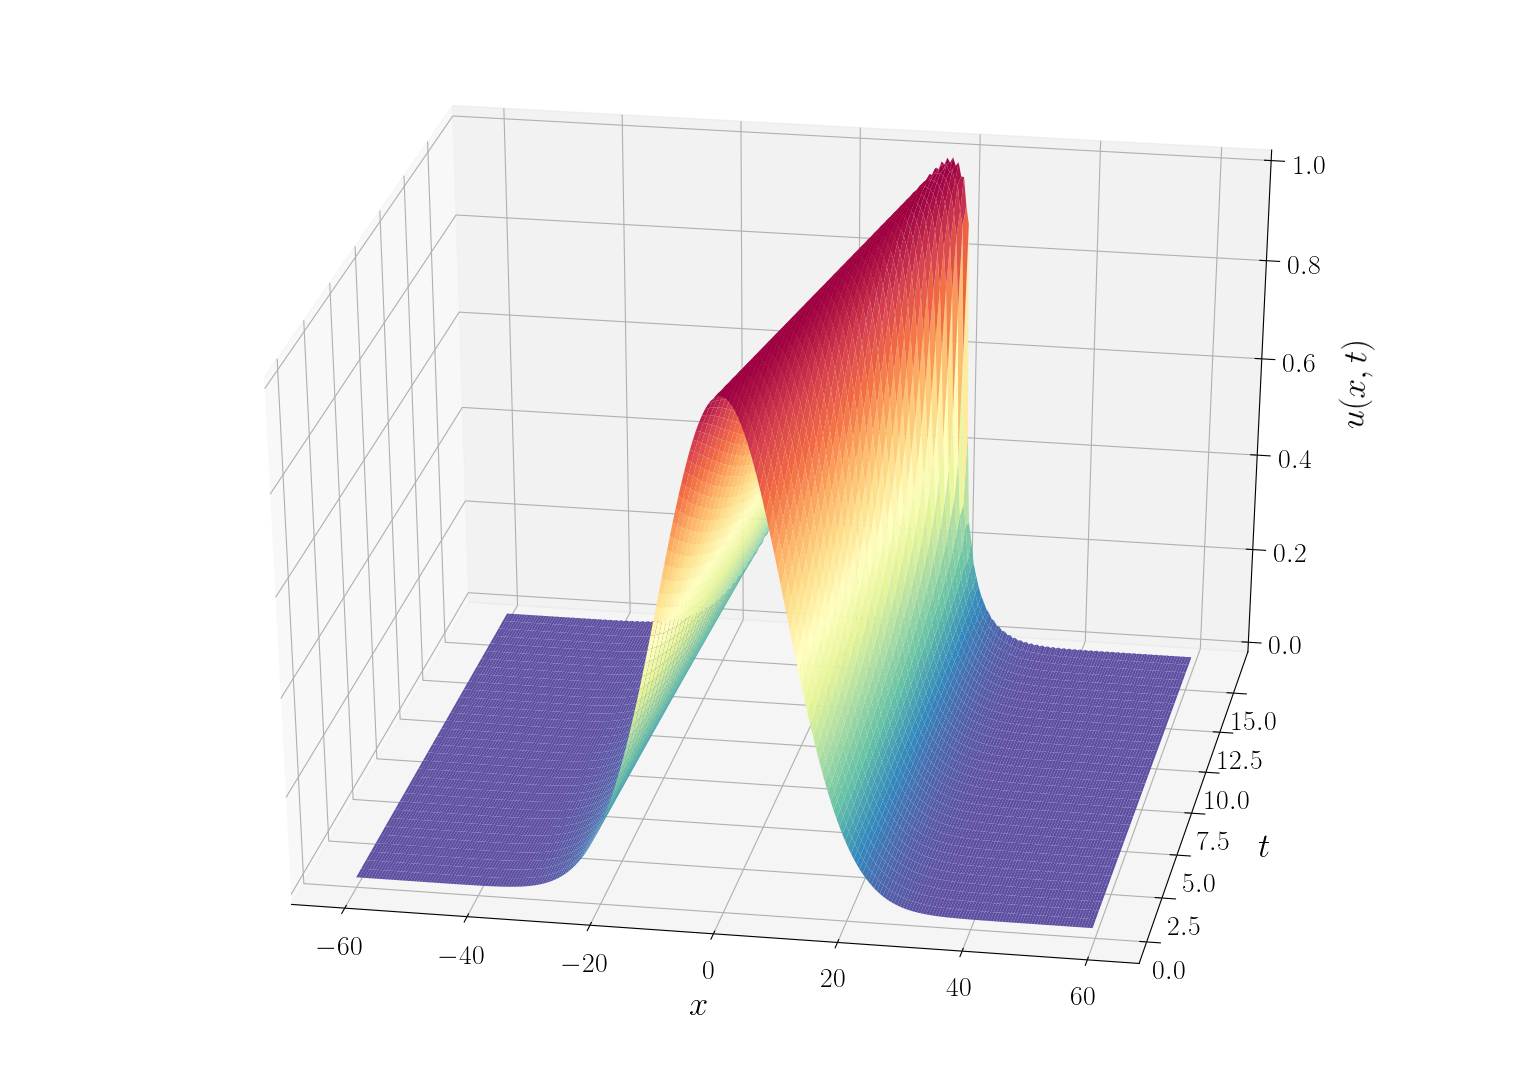
\includegraphics[width=12cm]{burgers_equation/deterministic/numerical_experiments/inviscid/figures/small_alpha.png}
		\caption{Numerical solution for (\ref{IVP_Burgers}) using (\ref{Galerkin_Euler}) with $\alpha = 1.0 \times 10^{-5}$, $N=256$, and $\Delta t = 1.0 \times 10^{-3}$.}
		\vspace{2mm}
		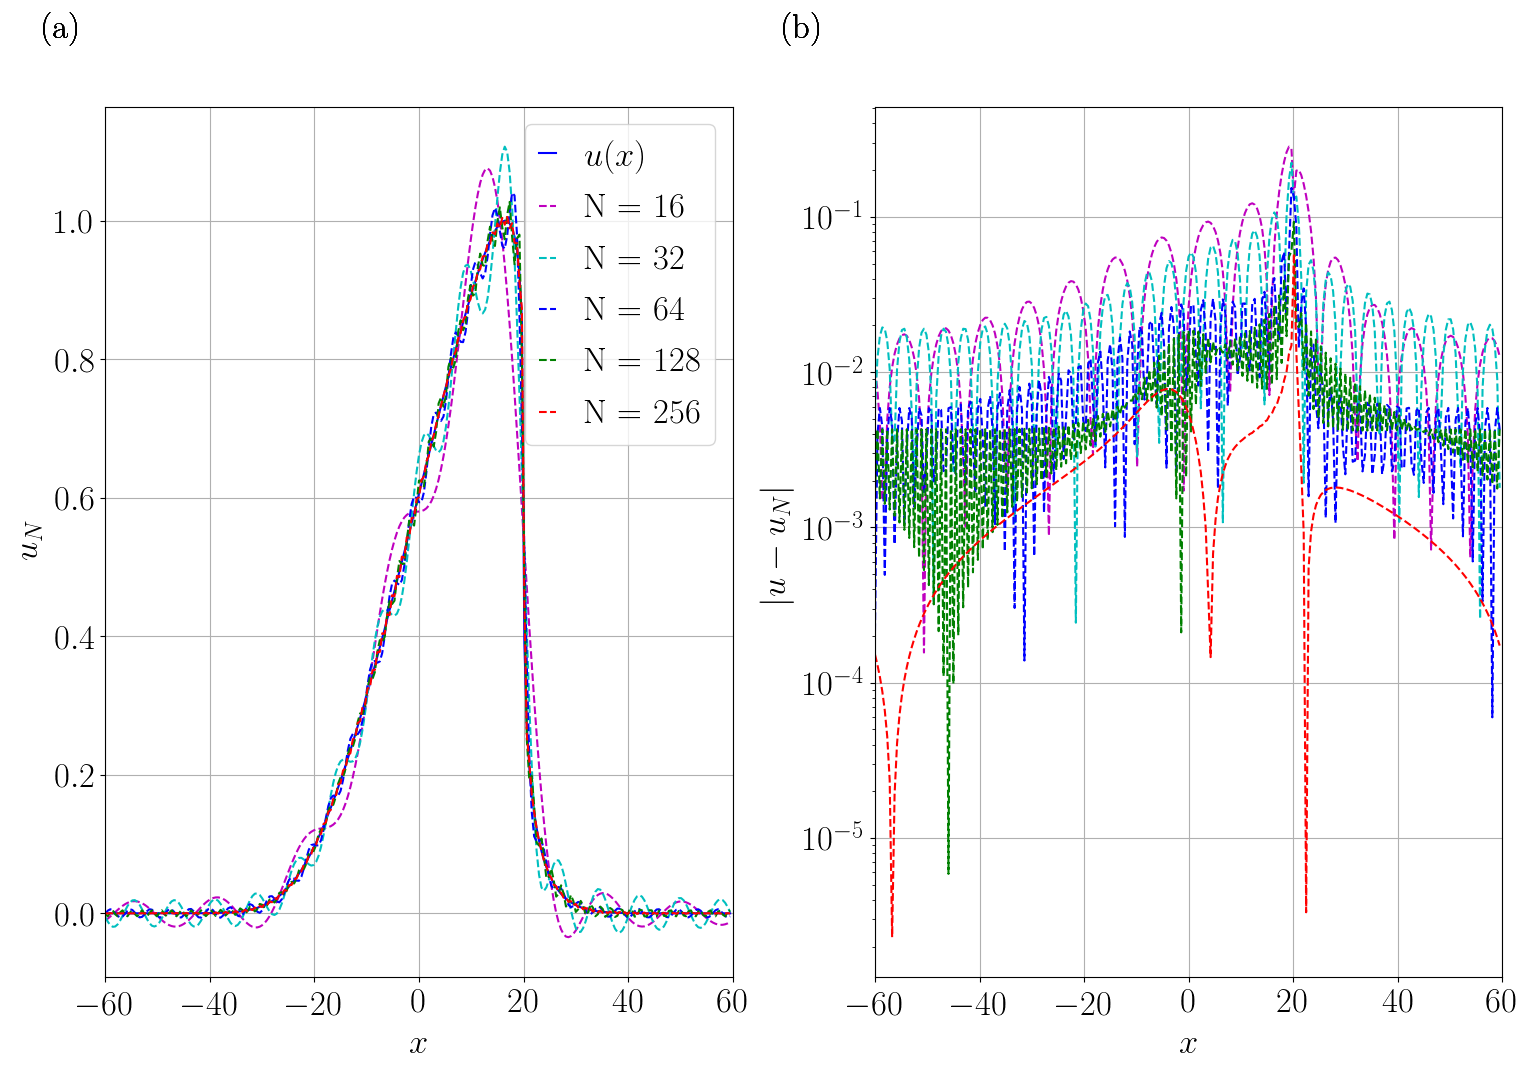
\includegraphics[width=12.5cm]{burgers_equation/deterministic/numerical_experiments/inviscid/figures/small_alpha_T.png}
		\caption{Numerical solution for (\ref{IVP_Burgers}) using (\ref{Galerkin_Euler}) at the time $T_c$ with $\alpha = 1.0 \times 10^{-5}$, and $\Delta t = 1.0 \times 10^{-3}$. (b) Point-wise error of approximation.}
	\end{figure}
	\newpage
	\begin{figure}[H]
		\centering	
		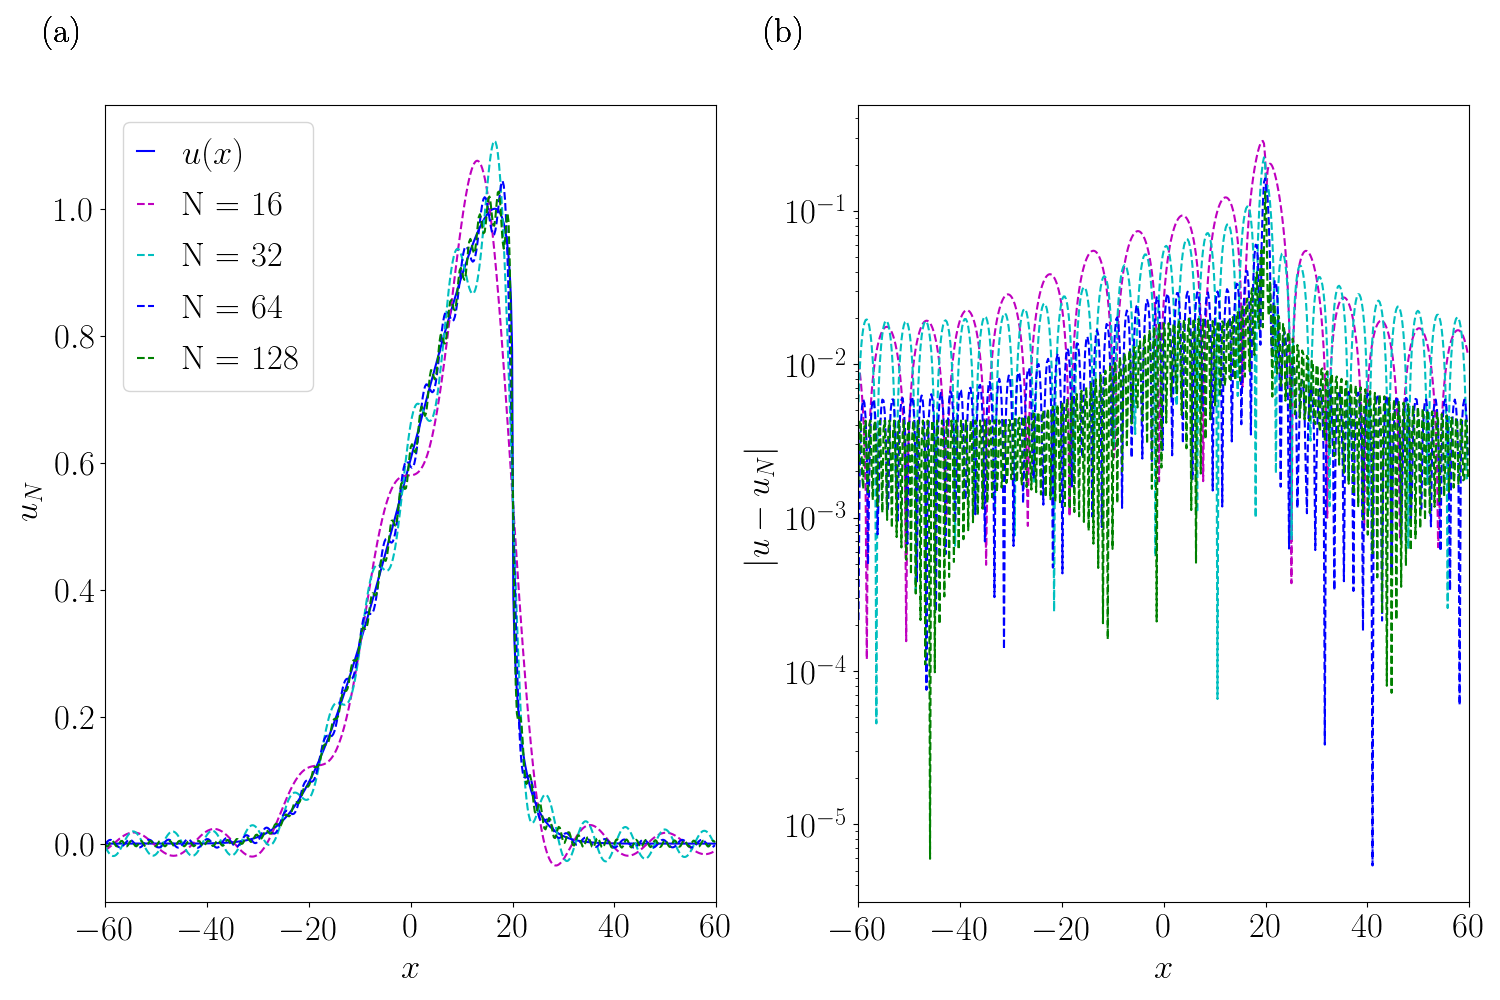
\includegraphics[width=13cm]{burgers_equation/deterministic/numerical_experiments/inviscid/figures/Numerical_Solution_Inviscid_T.png}
		\caption{(a) Exact solution for (\ref{IVP_Burgers}), and its approximations using (\ref{Galerkin_Euler}) at the time $Tc$ with initial condition $u_0(x) = e^{-0.005x^2}$, $x \in [-60, 60]$. (b) Pointwise error of approximation.}
		\label{convection_aprox_T}
		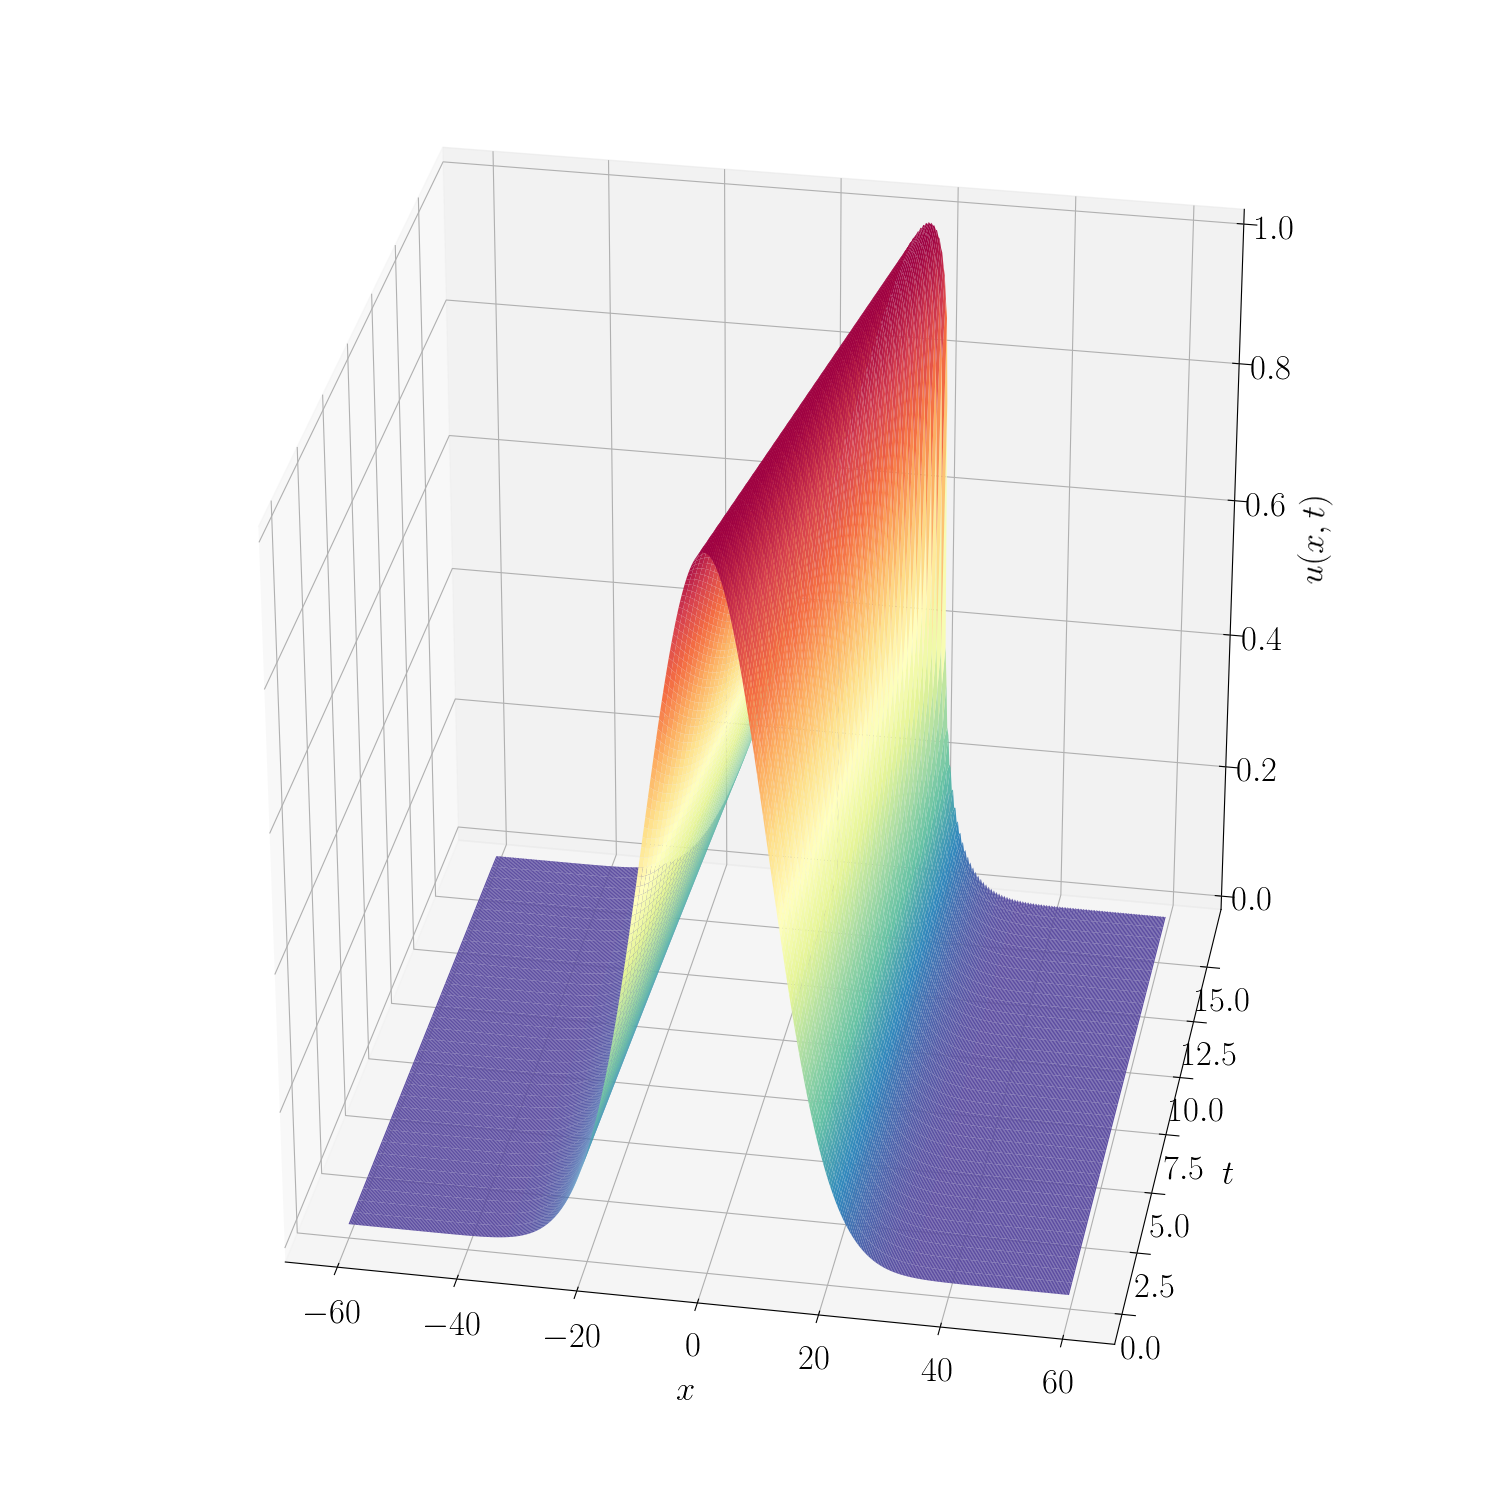
\includegraphics[width=11cm]{burgers_equation/deterministic/numerical_experiments/inviscid/figures/Numerical_Solution_Inviscid.png}
		\caption{Numerical approximation for  \ref{IVP_Burgers} using (\ref{Galerkin_Euler}) with $N=512$, $u_0(x) = e^{-0.005x^2}$, $x \in [-60, 60]$, and $t \in [0, Tc]$.}
	\end{figure}
	\newpage
	\begin{table}[H]
		\centering
		\begin{tabular}{lccc}
			\toprule
			\multicolumn{1}{c}{\hspace{6mm}\textbf{Expansion}} & \multicolumn{3}{c}{\textbf{Distance}} \\
			\hspace{12mm} $N$ & $\Delta t=1\times 10^{-2}$ & $\Delta t=1\times 10^{-3}$ & $\Delta t=1\times 10^{-4}$ \\
			\midrule
			\hspace{12mm} 16 & 0.285531 & 0.285732 & 0.285752 \\
			\midrule
			\hspace{12mm} 32 & 0.222737 & 0.223260 & 0.223312 \\
			\midrule
			\hspace{12mm} 64 & 0.160385 & 0.162782 & 0.163025 \\
			\midrule
			\hspace{12mm} 128 & 0.129297 & 0.133322 & 0.133733 \\
			\midrule
			\hspace{12mm} 256 & 0.083291 & 0.091449 & 0.092320 \\
			\bottomrule
		\end{tabular}
		\caption{Distance between exact solution for (\ref{IVP_Inviscid}) and the approximation for (\ref{IVP_Burgers}) with $\alpha = 1.0 \times 10^{-5}$.}
	\end{table}
	\begin{figure}[H]
		\centering
		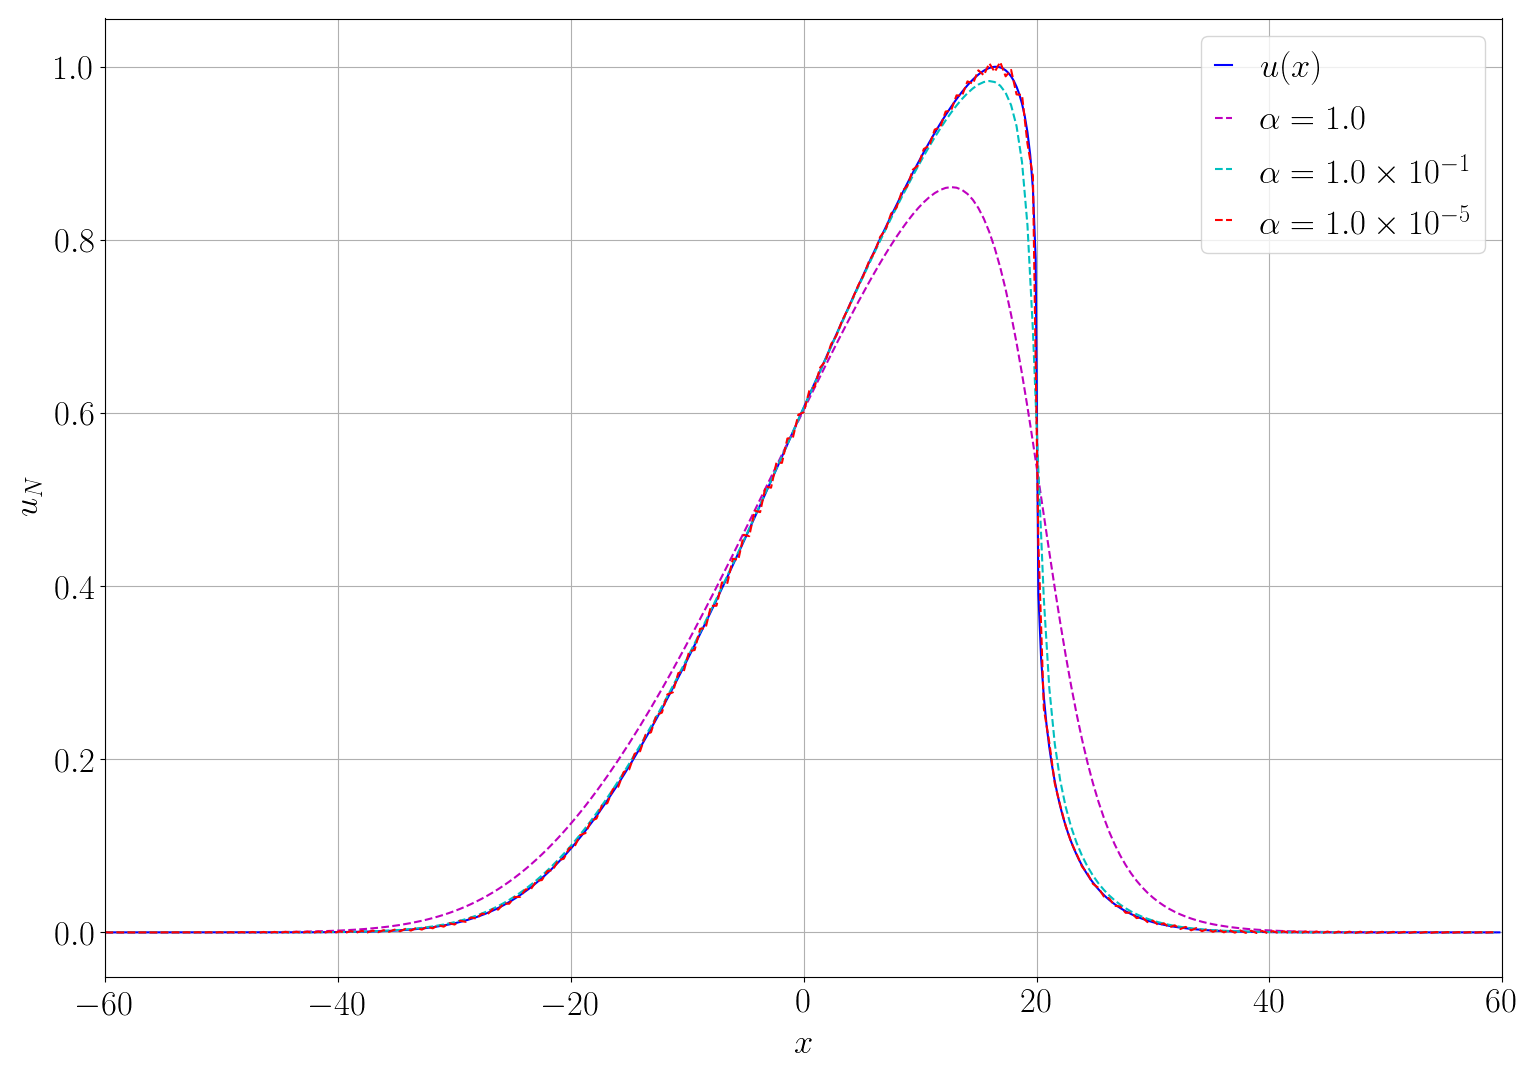
\includegraphics[width=12cm]{burgers_equation/deterministic/numerical_experiments/inviscid/figures/varios_alphas.png}
		\caption{Exact solution for (\ref{IVP_Inviscid}) and different approximations using (\ref{Galerkin_Euler}) with $N=256$, and $\Delta t = 1.0 \times 10^{-3}$.}
	\end{figure}
	
\chapter{Numerical Solutions for Burgers' equation in the Stochastic Version}
\label{Chapter_4}
	
	The objective of this chapter is to show how stochastic partial differential equations can be solved using spectral methods, for which it is much more difficult to find analytical or even numerical solutions. For this, we will dedicate the first section of this chapter to describe in the best possible way the details about a spectral method based on the Hermite series that has been studied in \cite{Delgado2016}, which associates a stochastic partial differential equation with the well-known equation Fokker-Planck-Kolmogorov, which is a partial differential equation that describes the time evolution of the probability density function of the velocity of a particle under the influence of random forces. \\

	We will use some results and definitions from the appendix \ref{Appendix_A} since the theoretical tools involved in the development of this method are outside the limitations of this work. This appendix contains the concepts necessary to understand the basic ideas of the method implementation that we will use in the second and last section considering the stochastic Burgers' equation that we have presented in (\ref{burgers_stochastic}). Finally, we will describe and show some numerical simulations. 

	\section{Spectral Approximation for Fokker-Plank-Kolmogorov Equation}

	The method that we are going to describe in this section will be developed in a space of Hilbert $\mathcal{H}$ with interior product $\langle \cdot, \cdot \rangle_{\mathcal{H}}$, where we will define a Gaussian measure $\mu$ with zero mean. Based on \cite{Delgado2016}, the Fokker-Planck-Kolmogorov equation is presented as follows
	\begin{align}
		\label{kolmogorov}
		\frac{\partial u}{\partial t} = \frac{1}{2} Tr(D^2 u) + \langle A(x), Du\rangle_{\mathcal{H}} + \langle B(x), Du\rangle_{\mathcal{H}}, \hspace{0.1cm} x \in D(A)
	\end{align}
	where $Tr$ is the trace operator, $A: D (A) \subset \mathcal{H} \rightarrow \mathcal{H}$ is a linear differential operator, $B: D (B) \subset \mathcal{H } \rightarrow \mathcal{H}$ is a nonlinear operator, and $D$ represents the Frechet derivative. \\
	
	The main idea of ​​the method is to solve the previous equation associating the following stochastic differential equation
	\begin{align}
		dX_t = AX_t dt + B(X_t) dt + dW_t
		\label{stochastic_equation}
	\end{align}
	where $W_t$ is a process $Q$-Wiener as defined in (\ref{cylindrical}), and the solution for the equation (\ref{kolmogorov}) is defined as follows
	\begin{align}
		u(x, t) = \mathbb{E} \left[ u_0 (X^x_t) \right] 
		\label{solution_kolmogorov}
	\end{align}
	where $u_0: \mathcal{H} \rightarrow \mathbb{R}$, and $X_t^x$ is the solution of the equation (\ref{stochastic_equation}). \\
	
	Following our reference, the solution to the problem (\ref{kolmogorov}) is represented by an expansion known as Fourier-Hermite which is given by the following series
	\begin{align}
		\label{infinite_approximation}
		u(x, t) = \displaystyle \sum_{n \in J} u_n (t) H_n (x), \hspace{2mm} x \in \mathcal{H}, \hspace{2mm} t \in [0, T],
	\end{align}  
	where $u_n : [0, T] \rightarrow \mathbb{R}$ and $H_n (x)$ are the Hermite functionals defined in \ref{hermite_funcionals}, and $J$ as in \ref{Conjunto_J}. \\
	  
	The above expansion can be justified by the Lemmas \ref{dense} and \ref{eigen}, and also is known as the deterministic Wiener-Chaos descomposition. Similarly, as we have seen in the previous chapter, it must satisfy the problem (\ref{kolmogorov}). For this, define the following operator
	\begin{align}
	\label{operator_L}
		\mathcal{L} u = \frac{1}{2} Tr(D^2 u) + \langle Ax, Du\rangle_{\mathcal{H}}, \hspace{2mm} x \in \mathcal{H}
	\end{align}
	which represents the linear part of (\ref{kolmogorov}), and by Lemma \ref{eigen} satisfies the following
	\begin{align}
		\label{Descomposition_L}
		\mathcal{L} u = - \sum_{n \in J} u_n (t) \lambda_n H_n (x).
	\end{align}	
	
	So, substituting the expansion on the left side of the equation (\ref{kolmogorov}) we get 
	\begin{align}
		\label{aprox_time}
		\frac{\partial u}{\partial t} = \displaystyle \sum_{n \in J}  \dot{u}_n (t) H_n (x),
	\end{align} 
	and for the non-linear term 
	\begin{align*}
		\langle B(x), Du\rangle_{\mathcal{H}} = \left\langle B(x), D_x \displaystyle \sum_{n \in J} u_n (t) H_n (x)  \right\rangle_{\mathcal{H}} 
	\end{align*}	
	\begin{align}
		\label{aprox_B}
		\hspace{8mm} = \displaystyle \sum_{n \in J} u_n (t) \left( B(x), D_x H_n (x) \right)_{\mathcal{H}}
	\end{align}
	
	Therefore, by (\ref{Descomposition_L} - \ref{aprox_B}) the equation (\ref{kolmogorov}) can be written as
	\begin{align*}
		\displaystyle \sum_{n \in J}  \dot{u}_n (t) H_n (x) = - \sum_{n \in J} u_n (t) \lambda_n H_n (x) + \sum_{n \in J} u_n (t) \left( B(x), D_x H_n (x) \right)_{\mathcal{H}}
	\end{align*}

	To develop the above, in the space $\mathcal{H}$ define the Gaussian measure $\mu (dx) = \frac{1}{\sqrt{2 \pi}} e^{- \frac{x^2 }{2}}$. So, multiplying the previous equation by $H_m (x)$, $m \in J$ and integrating over $\mathcal{H}$ with respect to the measure $\mu(dx)$ we have to
	\begin{align*}
		\displaystyle \sum_{n \in J}  \dot{u}_n (t) \int_{\mathcal{H}} H_m (x) H_n (x) \mu (dx) = &- \sum_{n \in J} u_n (t) \lambda_n \int_{\mathcal{H}} H_m (x)  H_n (x) \mu (dx) \\
		&+ \sum_{n \in J} u_n (t) \int_{\mathcal{H}} H_m (x) \left( B(x), D_x H_n (x) \right)_{\mathcal{H}} \mu (dx)
	\end{align*}
	and also using the orthogonality of the system $\{H_m (x) \}$, we get the following infinite system of coupled ordinary differential equations
	\begin{align}
		\label{infinite_system}
		\dot{u}_{m} (t) = -u_{m} (t) \lambda_{m} + \displaystyle \sum _{n \in \mathcal{J}} u_{n} (t) C_{n, m} , \hspace{2mm} n, m \in \mathcal{J}	
	\end{align}\textbf{}
	where $C_{n, m}$ is given by
	\begin{align}
		\label{Cnm}
		C_{n, m} = \displaystyle  \int_{\mathcal{H}} H_m (x) \left( B(x), D_x H_n (x) \right)_{\mathcal{H}} \mu (dx)
	\end{align} 

	We need to truncate and solve the above system to get approximations of the solution to the equation (\ref{kolmogorov}), which will be done in the next section focusing on the Burgers' equation given by (\ref{burgers_stochastic}).	
	\newpage
	\section{Numerical Solution for Burgers' Equation}
	Let $\mathcal{H} = L^2 (0, 1)$. Let's consider an initial value problem for (\ref{burgers_stochastic}) as follows
	\begin{align}
	\label{burgers_stochastic2}
	d X(\xi, t) = \left[\alpha \partial_{\xi}^2 X(\xi, t) + \frac{1}{2} \partial_\xi \left(X^2 (\xi, t)\right) \right] dt + dW_t (\xi, t), \hspace{0.2cm} \xi \in [0, 1] 
	\end{align}
	The boundary condition and its initial condition are respectively 
	\begin{align*}
	%\label{IC_burgers_stochastic2}
	X(0, t) &= X(1, t) = 0 , \hspace{0.2cm} t > 0 \\
	X(\xi, 0) &= x(\xi), \hspace{0.2cm}  x \in \mathcal{H},
	\end{align*}
	where $W$ is a cylindrical Wiener process on $\mathcal{H}$ as was given by \ref{cylindrical}, associated to a stochastic basis $(\Omega, \mathcal{F}, \mathbb{P}, \{\mathcal{F}_t\}_{t \geq 0})$, and as usually $\alpha > 0$ is the viscosity coefficient. \\
	
	Using the above problem, we will proceed to develop the implementation of the method described in the previous section.
	
	\subsection{Method Description and Its Implementation}
	
	\noindent We will denote the functions space that vanishes at the borders as $H^1_0 (0, 1)$. Setting $A = \alpha \partial^2_{\xi}$ and $B = \frac{1}{2} \partial_{\xi} (x^2)$, $x \in \mathcal{H}$, with its domains $D(A) = H^2 (0, 1) \cap H^1_0 (0, 1)$ and $D(B) = H^1_0 (0, 1)$ respectively, then by (\ref{stochastic_equation}), the equation (\ref{burgers_stochastic2}) can be rewritten as
	\begin{align*}
    	dX &= [AX + B(X)]dt + dW_t \\
        X(0) &= x, \hspace{0.2cm} x \in \mathcal{H}
	\end{align*}	
	where $A$  have eigenfunctions in $\mathcal{H}$ given by
	\begin{align*}
		e_k (\xi) = \sqrt{2} \sin{(k \pi \xi)}, \hspace{3mm} \xi \in [0, 1], \hspace{3mm} k \in \mathbb{N}
	\end{align*}
	
	\noindent Note that the operator $A$ satisfies $Ae_k = -\alpha \pi^2 k^2 e_k$ for $k \in \mathbb{N}$, then if we set $\Lambda = (-A)^{-1}$ we have that $\Lambda^{-1/2} e_k = \sqrt{2 \alpha} \pi |k| e_k$. \\	
				
	Therefore, as in (\ref{infinite_system}) we need to solve the following system
	\begin{align}
		\dot{u}_{m} (t) = -u_{m} (t) \lambda_{m} + \displaystyle \sum _{n \in \mathcal{J}} u_{n} (t) C_{n, m} , \hspace{0.1cm} n, m \in \mathcal{J}
	\end{align}
		
	\noindent We need to calculate the value of the constants $C_{n,m}$ , then we need to calculate expressions such as $B(x)$, $D_x H_n (x)$. Note that $x$ can be written as $x = \displaystyle \sum_{k} \beta_k e_k$ , with $\beta_k := \langle x, e_k \rangle_{\mathcal{H}}$. Then we have
	\begin{align*}
		B(x) = \frac{1}{2} \partial_{\xi} \left( \displaystyle \sum_k \beta_k e_k \right)^2 = \frac{1}{2} \partial_{\xi} \left[ \sum_l
		\sum_k \beta_l \beta_k e_l e_k \right] = \frac{1}{2} \sum_l
		\sum_k \beta_l \beta_k (e_l e'_k + e'_l e_k)
	\end{align*}
	and for $D_x H_n (x)$ we have
	\begin{align*}
		D_x H_n (x) = \displaystyle \sum_{j = 1}^{\infty} \prod_{i = 1. i \neq j}^{\infty} P_{n_i} (\langle x, \Lambda^{-1 / 2} e_i \rangle_{\mathcal{H}}) P'_{n_j} (\langle x, \Lambda^{-1 / 2} e_j \rangle_{\mathcal{H}}) \Lambda^{-1 / 2} e_j 
	\end{align*}
	
	\noindent Therefore, $C_{n, m}$ given by (\ref{Cnm}) gives
	\begin{align*}
		C_{n, m} =& \displaystyle \frac{1}{2} \int_{\mathcal{H}} H_m (x) \mu (dx) \sum_{j = 1}^{\infty} \prod_{i = 1, i \neq j}^{\infty} P_{n_i} (\langle x, \Lambda^{-1 / 2} e_i \rangle_{\mathcal{H}}) P'_{n_j} (\langle x, \Lambda^{-1 / 2} e_j \rangle_{\mathcal{H}})  \sqrt{2 \alpha} \pi |j| \\
		&\cdot \sum_l
		\sum_k \beta_l \beta_k (e_l e'_k + e'_l e_k) \\
		=& \displaystyle \frac{1}{2} \int_{\mathcal{H}} \mu (dx) \sum_{j = 1}^{\infty} \sqrt{2 \alpha} \pi |j| P_{m_j} (\langle x, \Lambda^{-1 / 2} e_j \rangle_{\mathcal{H}}) P'_{n_j} (\langle x, \Lambda^{-1 / 2} e_j \rangle_{\mathcal{H}}) \\  &\cdot \prod_{i = 1, i \neq j}^{\infty} P_{n_i} (\langle x, \Lambda^{-1 / 2} e_i \rangle_{\mathcal{H}}) P_{m_i} (\langle x, \Lambda^{-1 / 2} e_i \rangle_{\mathcal{H}}) \\
		&\cdot \sum_l
		\sum_k \beta_l \beta_k (e_l e'_k + e'_l e_k) 
	\end{align*}

	So, to obtain a truncated approximation of the solution, the following set of indices is considered
	\begin{align}
		J^{M, N} = \{\gamma = (\gamma_i, \hspace{1mm} 1 \leq \gamma_i \leq M  ) \hspace{1mm} | \hspace{1mm} \gamma_i \in \{0, 1, \cdots, N \} \}
	\end{align}
	this is the set of $M$-tuple which can take values in the set $\{0, 1, \cdots, N \}$. \\
	
	For $N_1 \in \mathbb{N}$ define as the set $S_{N_1} = \{n_1 , n_2 , \cdots , n_{N_1} : n_i \in J^{M,N} , i = 1, \cdots , N_1 \}$. Then for $n, m \in S_{N}$ we have 
	\begin{align*}
		\bar{C}_{n, m} =& \displaystyle \frac{1}{2} \sum_{j = 1}^{\infty} \sqrt{2 \alpha} \pi |j| \int_{\mathcal{\mathbb{R}^M}} P_{m_j} (\xi_j) P'_{n_j} (\xi_j) \mu (d \xi_j) \\  
		&\cdot \prod_{i = 1, i \neq j}^{M} P_{m_i} (\xi_i) P_{n_i} (\xi_i) \mu (d \xi_i) \sum_{l=1}^{M} \sum_{k=1}^{M} \beta_l \beta_k (e_l e'_k + e'_l e_k)
	\end{align*}

	and for $m_1, m_2, \cdots, m_M \in J^{M, N}$ the system (\ref{infinite_system}) give us
	\begin{align}
		\label{finite_system}
		\dot{u}_{m_i} (t) = -u_{m_i} (t) \lambda_{m_i} + \displaystyle \sum_{j=1}^{M} u_{n_j} (t) C_{n_j, m_i} , \hspace{2mm} 1 \leq i \leq M	
	\end{align}
	
	The solutions of the previous system can be calculated in terms of their eigenvectors by establishing the following vector
	\begin{equation*}
		U^M (t) =
		\begin{pmatrix}
			u_{m_1} (t) & u_{m_2} (t) & \dots & u_{m_M} (t)
		\end{pmatrix}^T   
	\end{equation*}
	and for its derivatives
	\begin{equation*}
		\dot{U}^M (t) =
		\begin{pmatrix}
			\dot{u}_{m_1} (t) & \dot{u}_{m_2} (t) & \dots & \dot{u}_{m_M} (t)
		\end{pmatrix}^T   
	\end{equation*}
	
	So, we can now write the system (\ref{finite_system}) as 
	\begin{align}
		\label{finite_system_vectorial}
		\dot{U}^M (t) = A U^M (t)
	\end{align}
	where the matrix $A$ is given by
	\begin{equation*}
		A =
		\begin{pmatrix}
			-\lambda_1 + C_{1,1} & C_{2,1} & \dots & C_{M-1,1} & C_{M,1} 
			\\
			C_{1,2} & -\lambda_2 + C_{2,2} & \dots & C_{M-1,2} & C_{M,2}  
			\\
			\vdots & \vdots & \ddots & \vdots & \vdots
			\\
			C_{1,M-1} & C_{2,M-1} & \dots & -\lambda_{M-1} + C_{M-1,M-1} & C_{M,M-1} 
			\\
			C_{1,M} & C_{2,M} & \dots & C_{M-1,M} & -\lambda_{M} + C_{M,M} 
		\end{pmatrix}
	\end{equation*}
	where $\lambda_i = \lambda_{mi}$ and $C_{i, j} = C_{n_i, m_j}$ para $1 \leq i, j \leq M$. \\
	
	\noindent Then, if $A$ has $M$ real and distint eigenvalues $\eta_i$ and $M$ eigenvectors $V_i$, then the solution to (\ref{finite_system_vectorial}) is given by
	\begin{align}
		\label{solution_finite_system}
		U^M (t) = \displaystyle \sum _{j = 1}^{M} c_i V_i e^{\eta_i t}
	\end{align}

	In the case when some eigenvalue is complex, we can write it together with its eigenvector as follows
	\begin{align*}
		V &= a + i b, \hspace{3mm} \eta = \beta + i \mu
	\end{align*}
	to get the solutions
	\begin{align*}
		e^{\beta t} (a \cos(\mu t) - b \sin(\mu t)), \hspace{2mm} e^{\beta t} (a \sin(\mu t) + b \cos(\mu t))
	\end{align*}
	which are real and different. \\
	
	Then we can write the approximation of the solution of (\ref{kolmogorov}) as
	\begin{align}
		\label{finite_approximation}
		u_M (x, t) = \displaystyle \sum_{ n \in J^{M, N} } u_n (t) H_n (x) = U^M (t) H^M (x), \hspace{2mm} x \in \mathcal{H}, \hspace{2mm}, t \in [0, T].
	\end{align}

	Also, if $u (\xi, t) = \mathbb{E} \left [X_t (\xi) \right]$, then satisfies the problem given by
	\begin{align*}
		\frac{\partial u}{\partial t} = \alpha \frac{\partial^2 u}{\partial \xi^2} + \partial_{\xi} \left[ u(\xi, t) \right]^2
	\end{align*}
	with the initial condition $u(\xi, 0) = \mathbb{E} \left[ X_0 \right]$. 
	\subsection{A Functional to obtain Initial Conditions}
	The interesting thing about the equation (\ref{kolmogorov}), is that there is no standard way to define an initial condition. For this problem, a functional is defined that acts in the initial condition, and because there are different ways of defining this functional, the method may change. For this work, the following functional was chosen 
	\begin{align*}
		u^{z_0}_0 (g) := g(z_0), \hspace{2mm} \text{for fixed} \hspace{2mm} z_0 \in [0, 1].
	\end{align*}
	
	To construct the initial condition, the following set of points is considered 
	\begin{align*}
		P = \{ z_i, \hspace{1mm} 0 \leq i \leq p \hspace{1mm} : \hspace{1mm} z_0 = 0, \hspace{1mm} z_p = 1 \}
	\end{align*}
	
	\noindent Then for each point $z_i \in P$ such that $X_0 (z_i) = X(0, z_i)$ set $u_0 (x)$ as the evaluation functional $z_i \longrightarrow X^x_t (z_i)$. Then from (\ref{solution_kolmogorov}) we obtain
	\begin{align}
		u(0, x) = \mathbb{E}[u^{z_i}_0 (X^x_0)] = X^x (0, z_i) = x(z_i)
	\end{align}
	For other hand
	\begin{align*}
		u (0, x) = \displaystyle \sum _{n \in \mathcal{J}^{M, N}} u_{n}(0) H_n (x)
	\end{align*}
	multiplying for $H_m (x)$ and integrating over space $\mathcal{L}^2 (\mathcal{H}, \mu)$ 
	\begin{align*}
		u_m (0) = \displaystyle \int_{\mathcal{H}} x(z_i) H_m (x) \mu (dx)
	\end{align*}
	
	\noindent Note that in the direction of the eigenfunction $e_k$ the expression $x$ can be written as $(x, e_k )_{\mathcal{H}} e_k$, then we can write $H_m (x) x (z_i)$ in the direction $e_k$ as $P_{m_k} (\xi_k) (x, e_k )_{\mathcal{H}} e_k (z_i)$ with $\xi_k = (x, \Lambda^{-\frac{1}{2}} e_k) = \| \lambda_k \| (x, e_k )_{\mathcal{H}}$ and $P_{m_k}$ is given by (\ref{hermite_polynomials}). Then we have
	\begin{align*}
		u^{z_i}_m (0) &= \displaystyle \int_{\mathcal{H}} x(z_i) H_m (x) \mu (dx) \\
		&= \int_{\mathbb{R}^N} \sum_{k=1}^{\infty} P_{m_k} (\xi_k) (x, e_k )_{\mathcal{H}} e_k (z_i) \mu (d\xi_1, d\xi_2, \cdots) e_k \\
		&= \int_{\mathbb{R}^N} \sum_{k=1}^{\infty} P_{m_k} (\xi_k) \frac{\xi_k}{\lambda_k} e_k (z_i) \mu (d\xi_1, d\xi_2, \cdots) e_k \\
		&= \sum_{k=1}^{\infty} \frac{e_k}{\lambda_k} \int_{\mathbb{R}}  P_{m_k} (\xi_k) \xi_k (z_i) \mu (d\xi_k)
	\end{align*}
	truncating the above expression we have
	\begin{align}
		\label{IC_approx}
		u^{z_i}_m (0) \approx \displaystyle \sum_{k=1}^{M} \frac{e_k}{\lambda_k} \int_{\mathbb{R}}  P_{m_k} (\xi_k) \xi_k (z_i) \mu (d\xi_k)
	\end{align} 
	
	\noindent Setting the equation (\ref{IC_approx}) for each element from $u^{z_i}_m$ as $u^{z_i}_{m_j} (0) = u_j (0)$, $1 \leq j \leq M$ and by (\ref{solution_finite_system}) evaluated for $t=0$, then the initial condition can be written as
	\begin{equation*}	
		\begin{pmatrix}
			u_1 (0) \\ u_2 (0) \\ \vdots \\ u_{M-1} (0) \\	u_M (0)
		\end{pmatrix}
		= 
		\begin{pmatrix}
			V1 & V2 & \dots & V_{M-1} & V_M
		\end{pmatrix}
		\begin{pmatrix}
			c_1 \\ c_2 \\ \vdots \\ c_{M-1} \\ c_M
		\end{pmatrix}
	\end{equation*}
	and the constants $c_j$ are calculated as
	\begin{equation*}
		\begin{pmatrix}
			c_1 \\ c_2 \\ \vdots \\ c_{M-1} \\ c_M 
		\end{pmatrix}
		=	
		\begin{pmatrix}
			V1 & V2 & \dots & V_{M-1} & V_M
		\end{pmatrix}^{-1}
		\begin{pmatrix}
			u_1 (0) \\ u_2 (0) \\ \vdots \\ u_{M-1} (0) \\	u_M (0)
		\end{pmatrix}
	\end{equation*}
	\subsection{Numerical Experiments}
    
    Now, we will proceed to describe the steps necessary to implement the method based on the above:
    \begin{enumerate}
    	\item We are going to consider the interval given by $[0, 1]$, which represents the domain of physical space, and similarly, the time will be set by the real value $t_f>0$ such that $[0, t_f]$. So, as a first step, we must define the problem well by choosing the parameters identified and required by the problem \ref{infinite_system}, which in the same way will be denoted by: $N$, $M$, $N_1 \in \mathbb{N}$, and $\alpha \in \mathbb{R}^+$.
    	
    	\item Given the above information, it is possible to follow the same methodology that we have analyzed in \ref{finite_system}, and define as a second step the calculation of the set $J^{M, N}$ given by \ref{Conjunto_J}, and then, as an intermediate step, obtain the set of points for each domain that we have defined above. 
    	
    	As an observation, the choice of the set of points, in this case, is arbitrary, and for example, We could obtain them by calculating the points $\xi_i \in [0, 1]$ defined for each $i = 0, 1, \dots, p \in \mathbb{N}^+$ as
    	\begin{align*}
    		\xi_i = \xi_0 + i \Delta \xi, \hspace{2mm} i = 0, 1, \dots, p
    	\end{align*}
    	and similarly for $t_j \in [t_0, t_f]$ with $j = 0, 1, \dots, l \in \mathbb{N}^+$ to obtain the following
    	\begin{align*}
    		t_j = t_0 + j \Delta t, \hspace{2mm} \Delta t = \frac{t_f - t_0}{l} 
    	\end{align*}
    	
    	\item Concluding with the previous steps will allow us to obtain everything that is required to begin to construct the initial value problem of the system \ref{finite_system_vectorial}, which could be considered as the step that requires more attention because we must obtain the matrix $\bar{C}_{n, m}$ using the simplification given in \ref{Cnm}. 
    	
    	However, this calculation gives the impression that it will give us a lot of work, but when observing its expression we can notice that we only have to focus on each of the combinations given by the multiplication of the Hermite polynomials that we must then integrate, for example, using some quadrature rule, and finally make its summation.
    	
    	\item Successfully achieving this last step, what remains are to solve an eigenvalue problem given by \ref{eigen}, which is solved by some conventional numerical method to obtain the eigenvalues $\eta_i$ with their respective eigenvectors $V_i$. 
    	
    	Then, Using the functional $u_0$ as in \ref{IC_approx} to calculate the constants $c_k$ for each $k = 1, \dots, M$, and by using the expansion given by \ref{solution_finite_system} to obtain the solution of the problem as follows

    	\begin{align*}
    		u^M(x_i, t_j) = \displaystyle \sum_{k=1}^{M} u_k (t_j) H_k (x_i), \hspace{2mm} \left\{x_i\right\}_{i=0}^{p} \in \left[ 0, 1 \right], \left\{t_j\right\}_{j=0}^{l} \in \left[ 0, t_f \right]
    	\end{align*}
    \end{enumerate}
    
    The following simulations that will be shown were performed using a discretization of $2048$ points in the spatial variable $\xi$ over the interval $[0, 1]$, and $1024$ points in the variable time $t$ over the interval $[0, 10]$. In addition, the values of the parameters $N = 5$, $M = 11$, and $\alpha = 1.0 \times 10^{-2}$ were considered. With this information, the solutions obtained were calculated using the following initial condition and its truncated Chebysheb expansion given by
    \begin{align*}
    	x(\xi) = \sin(\pi \xi), \hspace{3mm} y(\xi) = \displaystyle \sum^{N}_{k=0} c_k T_k (\xi),
    \end{align*}
    
    This numerical experiment consists of illustrating an interesting result given in \cite{Delgado2019}, which tells us that the solutions obtained from two close initial conditions also remain close. This behavior allows characterizing what is known as the stability of the approximation, and it is described by means of continuity with respect to the initial conditions of the numerical approximations of the equation (\ref{kolmogorov}). \\
    
    To understand this better, let us denote by $\Psi^{x}_t$ the solution of (\ref{kolmogorov}) obtained by
    \begin{align*}
    	u(x, t) = \mathbb{E} \left[ \varphi (X^x_t) \right]. 
    \end{align*}
    where $\varphi: \mathcal{H} \rightarrow \mathbb{R}$ is Lipschitz and $X^x_t$ is the solution to (\ref{stochastic_equation}) with initial conditions $X_0 = x \in \mathcal{H}$. So, as before, its expansion is given by
    \begin{align*}
    	\Psi^{x}_t = \displaystyle \sum _{n \in \mathcal{J}} u_n (t) H_n (x), \hspace{2mm} x \in \mathcal{H}, \hspace{2mm} t \in [0, T].
    \end{align*}
    
    Therefore, following our reference, the above is summarized as follows: Given two different initial conditions $x, y \in \mathcal{H}$, then we have the following estimate
	\begin{align*}
		\| \Psi^x_t - \Psi^y_t \|^2_{\left( L^2 (\mathcal{H}, \mu)\right)^2} \leq \exp(Ct) \displaystyle \int_{\mathcal{H} \times \mathcal{H}} \|x - y \|^2_{\mathcal{H}} \mu (dx) \mu (dy) + f(t) \|x - y\|_{\mathcal{H}},
	\end{align*}
	for some $C$ finite and $f(t)$ is given by
	\begin{align*}
		f(t) = \displaystyle \sum_{n \in J} \left[u^y_n (t)\right]^2 + \int_{\mathcal{H}} \mathbb{E}^2 \left[\varphi (X^y_t)\right] \mu (dy).
	\end{align*}	
	
	From the above, we can see that if $ \| x - y \|_{\mathcal{H}} \leq \delta$, so we have to $\| \Psi^x_t - \Psi^y_t \| \leq G (t) \delta$. As we have already mentioned, this continuity defines a type of stability for approximations, which is of utmost importance in this field since characterizations of this type are still under construction and are essential for the analysis of a numerical method. \\
	
	This behavior is shown in the following figures, which were obtained using codes that were created following the previous steps, and which can be found in \url{https://github.com/alanmatzumiya/Paper.git}. In figure \ref{IC_Cheb} it shows us the two initial conditions for which the equation (\ref{kolmogorov}) will be solved by associating it with (\ref{burgers_stochastic}), and in figure \ref{Stochastic_Solutions} we can see that the solutions keep the distance. Finally, the figure \ref{Continuity} shows the distances for each instant of time $t$, showing that they are actually getting closer as time passes.
	
\newpage
	\begin{figure}[H]	
		\centering	
		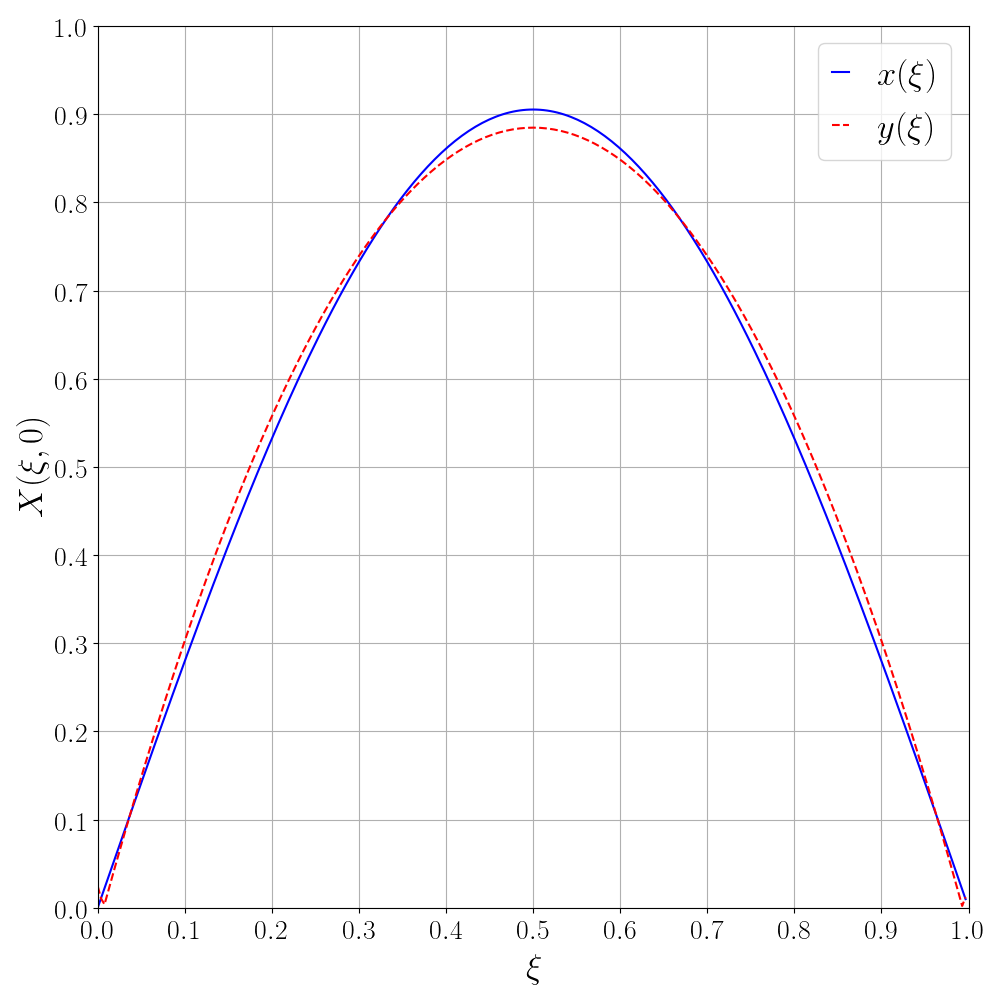
\includegraphics[width=.55\textwidth]{burgers_equation/stochastic/numerical_experiments/figures/IC.png}
		\caption{Initial condition for (\ref{burgers_stochastic2}) and its approximation.}
		\label{IC_Cheb}	
		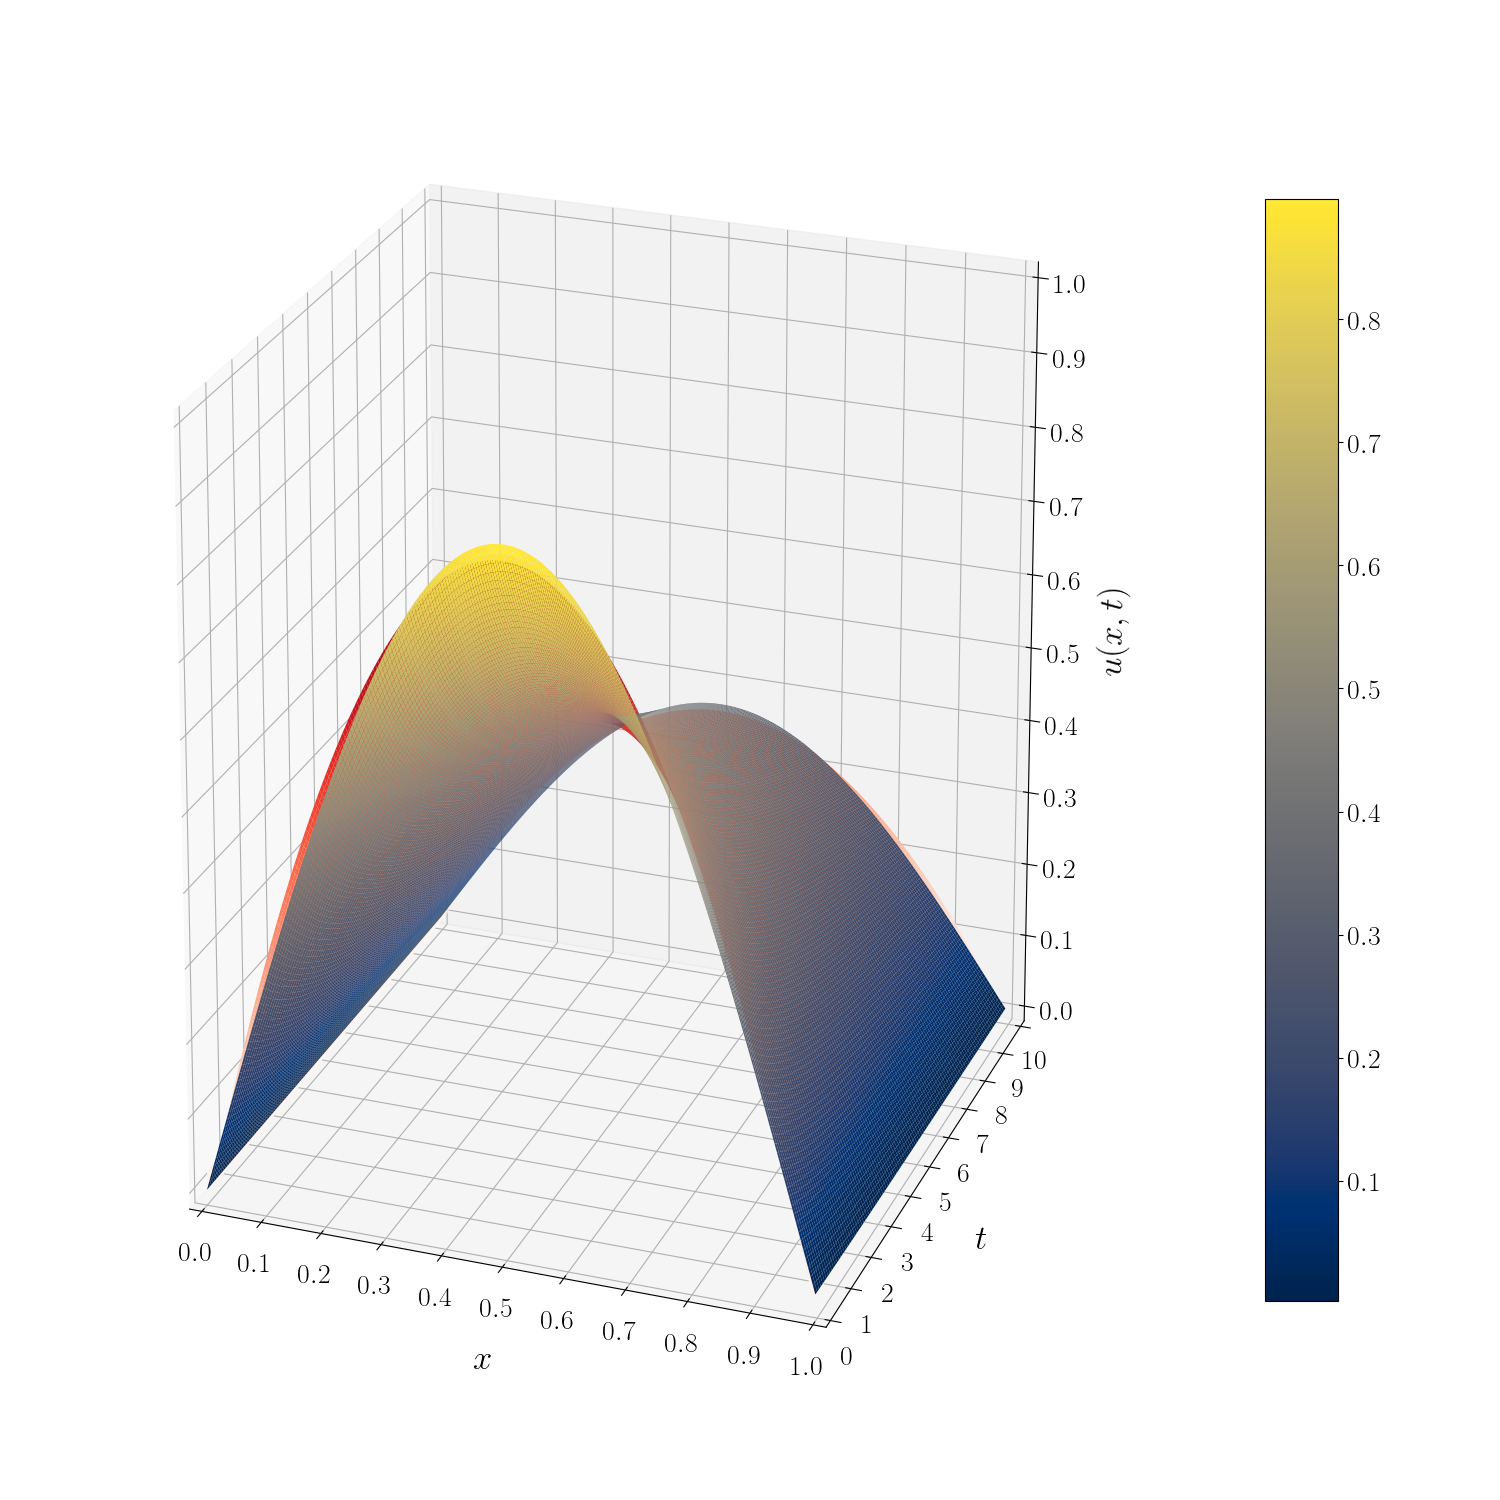
\includegraphics[width=.9\textwidth]{burgers_equation/stochastic/numerical_experiments/figures/Numerical_Solution_Stochastic.png}
		\caption{Numerical solutions for (\ref{burgers_stochastic2}) with initial conditions $x(\xi)$ and $y(\xi)$.}
		\label{Stochastic_Solutions}	
	\end{figure}
\newpage
	\begin{figure}[H]	
	\centering
		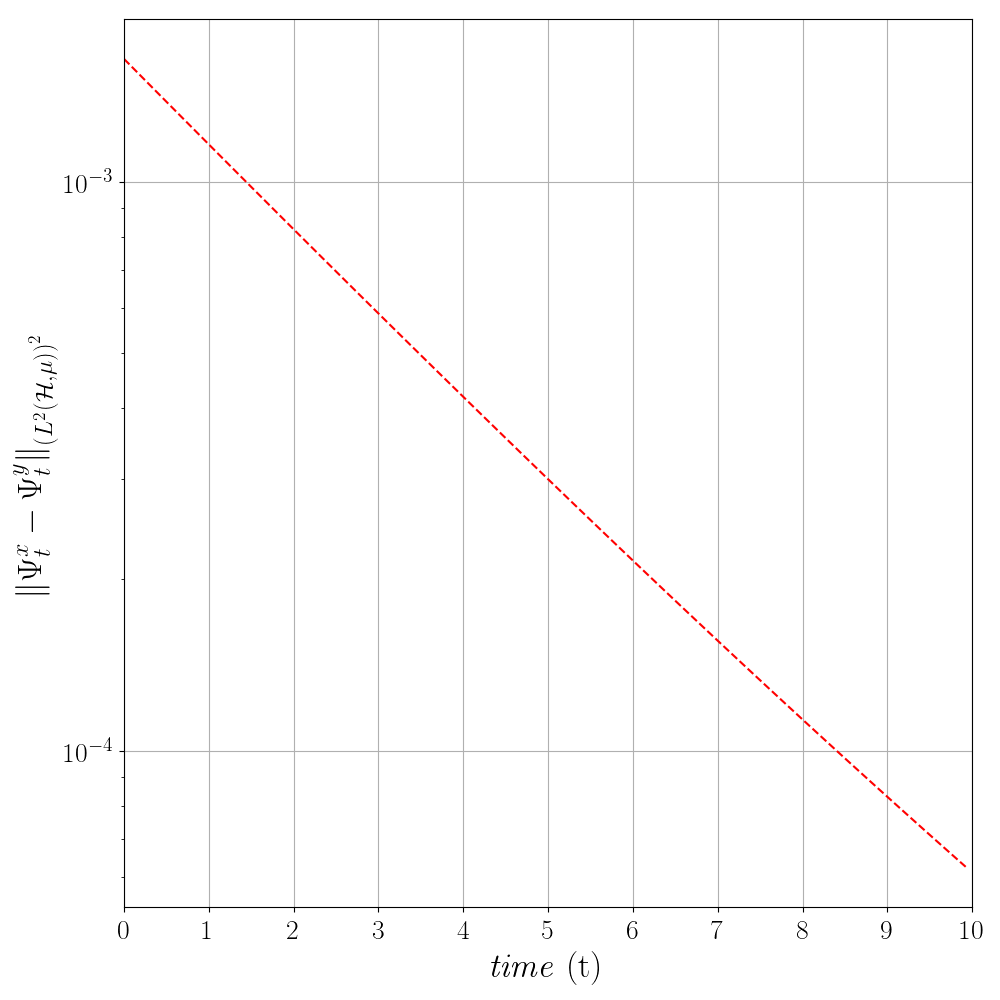
\includegraphics[width=.7\textwidth]{burgers_equation/stochastic/numerical_experiments/figures/norms.png}
		\caption{Distance between the numerical solutions for equation (\ref{burgers_stochastic2}) with initial conditions $x(\xi)$, and $y(\xi)$.}
		\label{Continuity}
	\end{figure}	

	
\chapter{Discussion and Conclusions}

	With what has been developed throughout this thesis work, it has given us a satisfactory understanding of the knowledge necessary to apply spectral methods in solving initial value problems of nonlinear partial differential equations, which with practice it will be possible to acquire the ability to study and attack other more complex problems. \\
	
	The practice that we have obtained when developing Chapter \ref{Chapter_3} with the help of the tools examined in Chapter \ref{Chapter_2}, can be useful to construct and study some other spectral method using another family of polynomials that allows us to approximate more precisely a function, and to construct practical methods for its implementation solving this same problem or another one of interest. Although, as expected based on theory, we were able to obtain good approximations using Fourier methods to solve linear problems. But, the situation was different when we considered the non-linear problem since it was not possible to obtain the solutions directly, forcing us to develop more carefully the numerical methods that finally gave us a good numerical approximation and with practical mathematical expressions for its implementation.  \\
	
	However, we noted that very small steps in time were required to ensure that the methods worked correctly, which greatly increased the computation time, but this was due to the presence of the aliasing error caused by the nonlinear term, which manifested itself unfavorably with small values of $\alpha$, and they should be handled more carefully, possibly considering another class of polynomials. Even so, we were able to satisfactorily detect the problems that can arise when using these tools, and it is interesting to delve into this with the help of the appropriate tools that allow us to characterize and know the convergence of these methods. \\
	
	Regarding the spectral method that we developed in the Chapter \ref{Chapter_4}, the problem that arises is due to the number of calculations that are necessary to obtain the numerical approximations, but nevertheless, the implementation is easy to understand and can be studied with more detail to propose a more efficient and less expensive algorithm to calculate, mainly attacking the calculation of the integrals involved in the process. For this type of problem, it is worth investigating an implementation that allows you to write parallel code in some programming language to optimize memory and computation times. \\
	
	Even so, it was possible to successfully carry out some numerical experiments that allowed us to observe a theoretical result that characterized the stability of this method, and perhaps could allow us to investigate other characteristics of interest, such as its convergence. Thanks to the practice developed in this chapter we have acquired the ability to implement a spectral method to carry out numerical studies that may be useful for its analysis, which could also be interesting to implement these same techniques in other problems that are considered important. \\
	
	Therefore, we can conclude that spectral methods are a good option to study partial differential equations, either deterministic or stochastic since in addition to giving us the possibility of obtaining good precision in their approximations provided they are implemented correctly, they are also an excellent alternative to investigate the nature of these problems, be they physical or mathematical, opening different paths, such as some of those already mentioned, that may be interesting for developing future research. \\
	
	Finally, from a personal perspective, it considers of great importance the knowledge about the use of programming languages to build quality algorithms, that is, that they manage to have a code structure that can be a base to solve other problems. In addition, good training in scientific computing is of great advantage when producing research on the development of algorithms that allow to satisfactorily show the precision of some numerical method, since it must be considered that this depends strongly on the quality of the computation and could interfere considerably with the evaluation of our experiments. 
	
	
	

\begin{appendices}
	\chapter{Elements of Probability}
\label{Appendix_A}
\section{Basic Definitions}
	\begin{definition}
		A probability measure $\mathbb{P}$ on a measurable space $(\Omega, \mathcal{F})$ is a function from $\mathcal{F}$ to $[0, 1]$ such that
			\begin{itemize}
				\item
				$\mathbb{P} (\emptyset) = 0$, and $\mathbb{P} (\Omega) = 1$.
				\item 
				If $\{ A_n \}_{n \geq 1} \in \mathcal{F}$ and $A_i \cap A_j \neq \emptyset$ if $i \neq j$, then $\mathbb{P} (\cup^{\infty}_{n=1} A_n) = \sum^{\infty}_{n = 1} \mathbb{P} (A_n)$.
			\end{itemize}	
	\end{definition}
	
	\noindent A $\sigma$-algebra on a set $X$ is a collection of subsets of $X$ that includes the empty subset and is closed under complement and under countable unions. Denote $\sigma (D) = \cap \{ H : H \text{ is a } \sigma \text{-algebra of } \Omega, D \subseteq H \}$. We call $\sigma (D)$ a $\sigma$-algebra generated by $D$.
	
	\begin{definition}
		A triple  $(\Omega, \mathcal{F}, \mathbb{P})$ is called a probability space if
		\begin{itemize}
			\item
			$\Omega$ is a sample space which is a collection of all samples.
			\item 
			$\mathcal{F}$ is a $\sigma$-algebra on $\Omega$.
			\item
			$\mathbb{P}$ is a probability measure on $(\Omega, \mathcal{F})$. 
		\end{itemize}	
	\end{definition}

	\noindent On a given probability space $(\Omega, \mathcal{F}, \mathbb{P}) (\Omega = \mathbb{R})$, if a cumulative distribution function of a random variable $X$ is normal, i.e.,
	\begin{align}
		\mathbb{P} (X < x) = \displaystyle \int_{-\infty}^{x} \frac{1}{ \sigma \sqrt{2 \pi} } e^{-\frac{(y - \mu)^2}{2 \sigma^2}} dy, \hspace{2mm} \sigma > 0,
	\end{align}
	then the random variable $X$ is called a Gaussian (normal) random variable on the probability space $(\Omega, \mathcal{F}, \mathbb{P})$. Here $X$ is completely characterized by its mean $\mu$ and its standard deviation $\sigma$. We denote $X \sim \mathcal{N} (\mu, \sigma^2)$. The probability density function of $X$ is
	\begin{align*}
		p(x) = \frac{1}{\sigma \sqrt{2 \pi}} e^{-\frac{(x - \mu)^2}{2 \sigma^2}}.
	\end{align*}

	\noindent When $\mu = 0$ and $\sigma = 1$, we call $X$ a standard Gaussian (normal) random variable.
	
	\begin{definition}
		A probability space $(\Omega, \mathcal{F}, \mathbb{P})$ is said to be a complete probability space if for all $B ∈\in \mathcal{F}$ with $\mathbb{P} (B) = 0$ and all $A \subseteq B$ one has $A \in \mathcal{F}$.
	\end{definition}
	
	\begin{definition}
		If $(\Omega, \mathcal{F}, \mathbb{P})$ is a given probability space then a function $Y : \Omega \rightarrow \mathbb{R}^n$ is called $\mathcal{F}$-measurable if $Y^{-1} (U) = \{ w \in \Omega : Y(w) \in U \} \in \mathcal{F}$ holds for all open sets $U \in \mathbb{R}^n$. If $X : \Omega \rightarrow \mathbb{R}^n$ is a function, then $\sigma (X)$ is the smallest $\sigma$-algebra on $\Omega$ containing all the sets $X^{-1} (U)$ for all open sets $U$ in $\mathbb{R}^n$.
	\end{definition}
	
	\begin{definition}
		Suppose that $(\Omega, \mathcal{F}, \mathbb{P})$ is a given complete probability space. A random variable $X$ is an $\mathcal{F}$-measurable function $X : \Omega \rightarrow \mathbb{R}^n$.
	\end{definition}
	
	\noindent Its well known that every random variable induces a probability measure $\mu_X$ (distribution of $X$) on $\mathbb{R}_n$ given by
	\begin{align*}
		\mu_X (B) = \mathbb{P} (X^{-1} (B)).
	\end{align*}
	If $ \int_{\Omega} | X(w) | d \mathbb{P} (w) < \infty$, the expectation of $X$ w.r.t. $\mathbb{P}$ is defined by
	\begin{align*}
		\mathbb{E} [X] = \int_{\Omega} X(w) d \mathbb{P} (w) = \int_{\mathbb{R}^n} x d \mu_X (x).
	\end{align*}  
	Also the $p$-th moment of $X$ is defined as (if the integrals are well defined)
	\begin{align*}
		\mathbb{E} [X^p] = \int_{\Omega} X^p d \mathbb{P} (w) = \int_{\mathbb{R}^n} x^p d \mu_X (x).
	\end{align*}
	The centered moments are defined by $\mathbb{E} \left[ |X - \mathbb{E}[X]| \right]$, $p = 1, 2, \dots, $. When
	$p = 2$, the centered moment is also called the variance. \\
	
	\begin{definition}
		Let $(\Omega, \mathcal{F}, \mathbb{P})$ be a probability space and let $T \subseteq \mathbb{R}$ be
		time. A collection of random variables $X_t$ , $t \in T$ with values in $\mathbb{R}$ is called a
		stochastic process. If time is an interval, $\mathbb{R}^+$ or $\mathbb{R}$, it is called a stochastic process with continuous time. For any fixed $w \in \Omega$, one can regard $X_t (w)$ as a function of
		$t$ (called a sample function of the stochastic process).
	\end{definition}

	\noindent On a probability space $(\Omega, \mathcal{F}, \mathbb{P})$, a filtration refers to an increasing sequence of $\sigma$-algebras:
	\begin{align*}
		\mathcal{F}_0 \subseteq \mathcal{F}_1 \subseteq \mathcal{F}_2 \subseteq \cdots \subseteq \mathcal{F}_n \subseteq \cdots .
	\end{align*}
	
	\noindent A natural filtration (w.r.t. $X$) is the smallest $\sigma$-algebra that contains
	information of $X$. It is generated by $X$ and $\mathcal{F}^X_n = \sigma(X_1, \dots, X_n)$ with $\mathcal{F}^X_0 = \{\emptyset, \Omega \}$. If $\lim_{n \rightarrow \infty} \mathcal{F}_n \subseteq \mathcal{F}$, then we call $(\Omega, \mathcal{F}, \{ \mathcal{F}_n \}_{n \geq 1}, \mathbb{P})$ a filtered probability space. A stochastic process $\{X_n \}$ on a filtered probability space is an adapted process if $X_n$ is $\mathcal{F}_n$-measurable for each $n$.
	
	\begin{definition}
		A family of sub-$\sigma$-algebras $\mathcal{F}_t \subseteq \mathcal{F}$ indexed by $t \in [0, \infty)$ is called a filtration if it is increasing $\mathcal{F}_s \subseteq \mathcal{F}_t$ when $0 \leq s \leq t < \infty$.
	\end{definition}
	
	\begin{definition} 
		A collection of random variables is called a Gaussian process, if the joint distribution of any finite number of its members is Gaussian. In other words, a Gaussian process is a $\mathbb{R}^d$-valued stochastic process with continuous time (or with index) $t$ such that $\left(X(t_0), X(t_1), \dots, X(t_n) \right)^T$ is a $(n+1)$-dimensional Gaussian random vector
		for any $0 \leq t_0 < t_1 < \cdots < t_n$. The Gaussian process is denoted as $X = \{X(t)\}_{t \in I}$ where $I$ is a set of indexes.
	\end{definition}
	
	\begin{definition}
		\label{brownian_motion}
		 A continuous time stochastic process $W(t)$ is called a standard Brownian motion if
		\begin{itemize}
			\item
			$W(t)$ is almost surely continuous in $t$, and $W(0) = 0$. 
			\item
			$W(t)$ has independent increments $W(t_{i+1}) - W(t_i)$ for all $t_n \geq 0$, $i = 0, 1, \dots, n$.
			\item
			$W(t) - W(s) \sim \mathcal{N} (0, t-s)$, i.e., obeys the normal distribution with mean zero and variance $t - s$.
		\end{itemize}	
	\end{definition}

	\noindent Set $x \in D \subset \mathbb{R}^d$, we define infinite dimensional Gaussian processes as follows
	\begin{align*}
		W^Q (x, t) = \displaystyle \sum^{\infty}_{j = 1} \sqrt{q_j} e_j (x) W_j (t),
	\end{align*}
	where $W_j (t)$ are mutually independent Brownian motions. Here $q_j \geq 0$, $j \in \mathbb{N}^d$ and $\{ e_j (x) \}$ is an orthonormal basis in $L^2 (D)$.  The following expansion is usually considered in literature:
	\begin{align*}
		\dot{W}^Q (x, t) = \displaystyle \sum^{\infty}_{j = 1} \sqrt{q_j} e_j (x) \dot{W}_j (t).
	\end{align*}
	where $\dot{W}_j (t) =\frac{d}{dt} W$, is formally the first-order derivative of $W_j (t)$ in time. When $q_j = 1$ for all $j$, we have a space-time white noise, and if $\sum^{\infty}_{j = 1} \sqrt{q_j}$ is called a $Q$-Wiener process. \\

	\noindent The Brownian motion and white noise can also be defined in terms of orthogonal expansions. Suppose that $\{e_j (t)\}_{j \geq 1}$ is a complete orthonormal system in $L^2 ([0, T ])$, then the Brownian motion $W(t)$ can be defined by
	\begin{align}
	    W(t) = \displaystyle \sum_{j=1}^{\infty} \beta_j \int_{0}^{t} e_j (s) ds, \hspace{2mm} t \in [0, T],
	\end{align}
	where $\beta_j$ are mutually independent standard Gaussian random variables for each $j$, and it can be also checked that is indeed a standard Brownian motion. Correspondingly, the white noise is defined by
	\begin{align}
	    \dot{W}(t) = \displaystyle \sum_{j=1}^{\infty} \beta_j e_j (t), \hspace{2mm} t \in [0, T].
    \end{align}

	\begin{definition}
		\label{cylindrical}
		Let $\{e_j\}_{j \geq 1}$ be a complete orthonormal  system of a separable Hilbert space $\mathcal{H}$, and $T \in \mathbb{R}^+$, and $\{\beta_j (t)\}_{j \geq 1}$ be an independent and identically distributed sequence of Brownian Motions. Then a cylindrical Wiener process $W$ in $\mathcal{H}$ is given by
		\begin{align*}
			W(t) = \displaystyle \sum_{j=1}^{\infty} \beta_j e_j (t)
		\end{align*}	
	\end{definition}
	
	\section{Some Important Results in Probability Spaces}
	
	
	It is well known that the Hermite Polynomials $\{P_k (\dot) \}_{k \in \mathbb{N}}$ with $P_0 = 1$ is a complete orthonormal system for $L_2 (\mathbb{R}, \mu_1 (dx))$ with $\mu_1 (dx) = \frac{1}{\sqrt{2 \ pi}} e^{- \frac{x^2}{2}} dx$, which are defined by 
	\begin{align}
		\label{hermite_polynomials}
		P_k(x) = \frac{(-1)^k}{(k!)^{1/2}} e^{\frac{x^2}{2}} \frac{d^k}{dx^k} e^{-\frac{x^2}{2}}, \hspace{3mm} x \in \mathbb{R}
	\end{align}
	
	
	A functional $\Phi: \mathcal{H} \longrightarrow  \mathbb{R}$, is said to be a smooth simple functional (or a cylinder functional) if there exists a $C^{\infty} $-function $\varphi$ on $\mathbb{R}^n$ and $n$-continuous linear functional $l_1 ,\cdots ,l_n$ on $\mathcal{H}$ such that for $h \in \mathcal{H}$
	\begin{align*}
		\Phi(h) = \phi(h_1, \cdots, h_n) \hspace{2mm} \text{where} \hspace{2mm} h_i = l_i (h), \hspace{2mm} i = 1, \cdots, n.
	\end{align*}
	
	Let $\mathbb{H} = L_2 (\mathcal{H}, \mu)$ denote the Hilbert space of Borel measurable functionals on the probability space with inner product
	\begin{align}
		\label{Inner_Functionals}	
		\langle \Phi, \Psi \rangle_{\mathbb{H}} = \displaystyle \int_{\mathcal{H}} \Phi (v) \Psi (v) \mu (dx), \hspace{2mm} \Phi, \Psi \in \mathbb{H},
	\end{align}
	and the norm $\| \Phi \|_{\mathbb{H}} = \langle \Phi, \Phi\rangle_{\mathbb{H}}^{1/2}$. In $\mathcal{H}$ we choose a basis system $\{\varphi_k \}$ such that $\varphi_k \in \mathcal{H}$.\\	
	
	Let $\Lambda$ an operator such that $Tr < +\infty$. We will denote as $\mathcal{H}_0$ the Hilbert subspace of $\mathcal{H}$ with inner product $\langle g, h \rangle_0 = \langle \Lambda^{1/2} g, \Lambda^{1/2} h \rangle_{\mathcal{H}}$ for $g, h \in \Lambda^{1/2} \mathcal{H}$, which is the completion of $\Lambda^{1/2} \mathcal{H}$ with respect to the norm $\| g \|_0 = \langle g, g \rangle^{1/2}$, and also is dense in $\mathcal{H}$. Then, by using the above can be defined The Hermite functional as follows
	\begin{align}
	\label{hermite_funcionals}
		H_n(h) = \prod_{i=1}^{\infty} P_{n_i} (l_i (h)), h \in \mathcal{H}_0 , n \in J
	\end{align}
	with
	\begin{equation*}
		l_i (h) = \left\langle h, \Lambda^{-1/2} \varphi_i \right\rangle_{\mathcal{H}}, \hspace{3mm} i = 1,2 \cdots
	\end{equation*}
	and the set $\mathcal{J}$ is given by
	\begin{align}
	\label{Conjunto_J}	
		\mathcal{J} = \{\alpha = (\alpha_i,i \geq 1) | \alpha_i \in \mathbb{N}\cup {0}, |\alpha|:= \displaystyle \sum _{i = 0}^{\infty}\alpha_i < \infty\}
	\end{align}
	

	\begin{lemma}
	\label{dense}	
		For $h \in \mathcal{H}$ let $l_i (h) = (h, \Lambda^{-1/2} \varphi_i )_{\mathcal{H}}$, $i=1, 2, \cdots$. Then the set $\{H_n \}$ of all Hermite polynomials on $\mathcal{H}$ forms a complete orthonormal system for $\mathbb{H}$. Hence the set of all functionals are dense in $\mathbb{H}$. Moreover, we have the direct sum decomposition:
		\begin{align*}
		\mathbb{H} = \displaystyle \bigoplus^{\infty}_{j=0} K_j,
		\end{align*}
		where $K_j$ is the subspace of $\mathbb{H}$ spanned by $\{H_n : |n| = j \}$. This result can be found in \cite{DAPRATO1994}.
	\end{lemma}


	\begin{lemma}
		\label{eigen}
		Let $H_n (h)$ be a Hermite polynomial functional given by (\ref{hermite_funcionals}), and suppose that the operator $-A$ have eigenfunctions $e_k$ with eigenvalues $\lambda_k$. Then the operator given in (\ref{operator_L}) satisfies the following
		\begin{align}
			\label{eigen_lambda_kolmo}
			\mathcal{L} H_n (h) = - \lambda_n H_n (h)
		\end{align}
		for any $n \in \mathcal{J}$ and $H_n \in \mathcal{H}$, where
		\begin{align*}
			\lambda_n = \displaystyle \sum_{k=1}^{\infty} n_k \lambda_k
		\end{align*}
	\end{lemma}
\end{appendices}

%\include{computational_studies}

%\include{appendix}

\backmatter

\bibliographystyle{plain}
%\addcontentsline{toc}{chapter}{\numberline{}Bibliograf\ia{}a}%
% Encoding: UTF-8

\begin{thebibliography}{X}

\bibitem{Delgado2016} Delgado Vences, Francisco \& Flandoli, Franco. (2016). A spectral-based numerical method for Kolmogorov equations in Hilbert spaces. Infinite Dimensional Analysis, Quantum Probability and Related Topics. 10.1142/S021902571650020X. 

\bibitem{Acheson2001} Acheson, D. J. Elementary Fluid Dynamics. Clarendon Press, 2001.

\bibitem{Batchelor1967} Batchelor, G. K. An Introduction to Fluid Dynamics, By G.K. Batchelor. 1967.

\bibitem{Landau1987} Landau, Lev D., and Lif$\v{s}$ic Evgenij M. Fluid Dynamics. Pergamon, 1987.

\bibitem{Currie1974} Currie, Iain G. Fundamental Mechanics of Fluids. McGraw-Hill, 1974.

\bibitem{Temam1984} Temam, Roger. Navier-Stokes Equations: Theory and Numerical Analysis. North-Holland, 1984.

\bibitem{Bateman1915} Bateman, H. (1915) Some Recent Researches on the Motion of Fluids. Monthly Weather Review, 43, 163-170. http://dx.doi.org/10.1175/1520-0493(1915)43$<$163:SRROTM$>$2.0.CO;2

\bibitem{Burgers1939} J M Burgers,Trans. R. Netherlands Acad. Sci. Amster-dam17, 1 (1939)

\bibitem{Burgers1948} J M Burgers,Adv. Appl. Mech.1, 171 (1948)

\bibitem{Schwartz1966} Schwartz, Laurent. Theorie Des Distributions. Hermann, 1966.

\bibitem{Lions1972} Lions, J.-L, and Enrico Magenes. Non-Homogeneous Boundary Value Problems and Applications. Springer-Verlag, 1972.

\bibitem{Renardy1993} Renardy, Michael, and Robert C. Rogers. An Introduction to Partial Differential Equations. Springer, 1993.	

\bibitem{Hopf1950} E Hopf,Commun. Pure Appl. Math.3, 201 (1950)

\bibitem{Cole1951} J D Cole,Quart. Appl. Math.9, 225 (1951)

\bibitem{Chambers1988} Chambers, D. H., et al. “Karhunen–Loéve Expansion of Burgers’ Model of Turbulence.” Physics of Fluids, vol. 31, no. 9, 1988, pp. 2573–2582., doi:10.1063/1.866535.

\bibitem{CHOI1992} H. CHOI, R. TEMAM, P. MOIN, J. KIM, Feedback control for unsteady flow and its application to Burgers equation, Center for Turbulence Research, Stanford University, CTR Manuscript 131. To appear on J. Fluid Mechanics (1992)

\bibitem{DAH-TENC1969} DAH-TENC JENG Forced Model Equation for Turbulence, The Physics of Fluids 12, 10, 2006-2010 (1969)

\bibitem{HOSOKAWA1975} I. HOSOKAWA, K. YAMAMOTO, Turbulence in the randomly forced one dimensional Burgers flow, J. Stat. Phys. 13, 245 (1975)

\bibitem{KARDAR1986} M. KARDAR, M. PARISI, J. C. ZHANG Dynamical scaling of growing interfaces, Phys. Rev. Lett. 56, 889 (1986)

\bibitem{KHANIN2007} J. Bec; K. Khanin. Burgers turbulence. Phys. Rep. 447 (2007), 1–2, 1–66.

\bibitem{WEINAN} E. Weinan. Stochastic hydrodynamics. Current developments in mathematics, 2000, 109–147, Int. Press, Somerville, 2001.

\bibitem{BERTINI1994} L. Bertini ;N. Cancrini ;G. Jona–Lasinio. The stochastic Burgers equation. Comm. Math. Phys. 165 (1994), 2, 211–232.

\bibitem{Catuogno2014} P. Catuogno ;C. Olivera. Strong solution of the stochastic Burgers equation. Appl. Anal. 93 (2014), 3, 646–652.

\bibitem{DAPRATO1994} G. Da Prato ; A. Debussche ; R. Temam. Stochastic Burgers equation. NoDEA Nonlinear Differential Equations Appl. 1 (1994), 4, 389–402.

\bibitem{PERKOWSKI2015} M. Gubinelli ; N. Perkowski Lectures on singular stochastic PDEs , Ensaios Matemáticos, 29. Sociedade Brasileira de Matemática, Rio de
Janeiro, 2015.

\bibitem{Canuto2012} Canuto, Claudio and Hussaini, M Yousuff and Quarteroni, Alfio Maria and Thomas Jr, A and others, Spectral methods in fluid dynamics. Springer Science \& Business Media (2012) 2017.06.28

\bibitem{Burges1995} F T Nieuwstadt and J A Steketee, Selected papers of J M Burgers(Springer Science+Business Media, BV,Dordrecht, 1995)

\bibitem{gottlieb2007} Hesthaven, Jan S. and Gottlieb, Sigal and Gottlieb, David, Spectral Methods for Time-Dependent Problems. Cambridge Monographs on Applied and Computational Mathematics (2007) 10.1017/CBO9780511618352

\bibitem{Richtmyer1968} I., E., Richtmyer, R. D., and Morton, K. W. (1968). Difference Methods for Initial-Value Problems. Mathematics of Computation, 22(102), 465. doi: 10.2307/2004698

\bibitem{KATO} KATO, Tosio. Fractional powers of dissipative operators. J. Math. Soc. Japan 13 (1961), no. 3, 246--274. doi:10.2969/jmsj/01330246. https://projecteuclid.org/euclid.jmsj/1261062709

\bibitem{LASIECKA} Lasiecka, I. (1984). Convergence Estimates for Semidiscrete Approximations of Nonselfadjoint Parabolic Equations. SIAM Journal on Numerical Analysis, 21(5), 894–909. doi:10.1137/0721058 

\bibitem{Kruzkov1970} S N Kružkov, "FIRST ORDER QUASILINEAR EQUATIONS IN SEVERAL INDEPENDENT VARIABLES", MATH USSR SB, 1970, 10 (2), 217–243 

\bibitem{Tadmor1989} Eitan Tadmor. 1989. Convergence of spectral methods for nonlinear conservation laws. SIAM J. Numer. Anal. 26, 1 (February 1989), 30–44. DOI:https://doi.org/10.1137/0726003

\bibitem{Maday1989} Yvon Maday and Eitan Tadmor. 1989. Analysis of the spectral vanishing viscosity method for periodic conservation laws. SIAM J. Numer. Anal. 26, 4 (August 1989), 854–870. DOI:https://doi.org/10.1137/0726047

\bibitem{Delgado2019} Delgado Vences, Francisco \& Matzumiya-Zazueta, Alan \& Saul, Diaz-Infante. (2019). INITIAL CONDITIONS CONTINUITY OF A NUMERICAL APPROXIMATION FOR KOLMOGOROV EQUATIONS *. 10.13140/RG.2.2.21593.47203.

\end{thebibliography}

\end{document} 